\documentclass[10pt]{article}
% ================================================================================
\usepackage{tikz}
\usepackage{array}
\usepackage{tabto}
\usepackage{float}
\usepackage[table,xcdraw]{xcolor}
\usepackage{caption}
\usepackage{amsmath}
\usepackage{amssymb}
\usepackage{hyperref}
\usepackage{multicol}
\usepackage{inputenc}
\usepackage{amsfonts}
\usepackage{graphicx}
\usepackage{listings}
\usepackage{titlesec}
\usepackage{fancyhdr}
\usepackage{subcaption}
\usepackage{stackengine}
\usepackage{smartdiagram}
\usepackage{pythonhighlight}
\usepackage{stfloats}
\usepackage{CJKutf8}
% Bar chart drawing library 
\usepackage{pgfplots} 
% ================================================================================
\setcounter{secnumdepth}{4}
\titleformat{\paragraph}
{\normalfont\normalsize\bfseries}{\theparagraph}{1em}{}
\titlespacing*{\paragraph}
{0pt}{3.25ex plus 1ex minus .2ex}{1.5ex plus .2ex}
\hypersetup{
    colorlinks=true,
    linkcolor=blue,
    filecolor=magenta,      
    urlcolor=red,
    pdftitle={Overleaf Example},
    pdfpagemode=FullScreen,
    }
\setlength{\topmargin}{-.5in} \setlength{\textheight}{9.25in}
\setlength{\oddsidemargin}{0in} \setlength{\textwidth}{6.8in}
% ================================================================================
\newcounter{mycounter} 
\newcommand\showmycounter{\stepcounter{mycounter}\themycounter}
\newcommand\showlips{\stepcounter{mycounter}\lipsum[\value{mycounter}]}
% ================================================================================
\definecolor{codegreen}{rgb}{0,0.6,0}
\definecolor{codegray}{rgb}{0.5,0.5,0.5}
\definecolor{codepurple}{rgb}{0.58,0,0.82}
\definecolor{backcolour}{rgb}{0.95,0.95,0.92}
% ================================================================================
\lstdefinestyle{mystyle}{
    backgroundcolor=\color{backcolour},   
    commentstyle=\color{codegreen},
    keywordstyle=\color{magenta},
    numberstyle=\tiny\color{codegray},
    stringstyle=\color{codepurple},
    basicstyle=\ttfamily\footnotesize,
    breakatwhitespace=false,         
    breaklines=true,                 
    captionpos=b,                    
    keepspaces=true,                 
    numbers=left,                    
    numbersep=5pt,                  
    showspaces=false,                
    showstringspaces=false,
    showtabs=false,                  
    tabsize=2
}
\lstset{style=mystyle}
% ================================================================================
\graphicspath{{images/}}
% \usepackage[includefoot]{geometry}
% \usepackage{blindtext}
% \usepackage{lastpage}
% \usepackage{fancyhdr}
% \pagestyle{fancy}
% \fancyhf{} % clear existing header/footer entries
% % Place Page X of Y on the right-hand
% % side of the footer
% \fancyfoot[R]{Page \thepage \hspace{1pt} of \pageref{LastPage}}
% ================================================================================
\pagenumbering{arabic}
% \usepackage{lastpage}

% \usepackage{fancyhdr}

% \fancyfoot[C]{Page \thepage\ of \pageref{LastPage}}

\pagestyle{fancy}

\title{Title}
% \author{Group Hololive' Face Detection}
\fancyhf{}
\fancyfoot[C]{\thepage}
\lhead{\bfseries Vietnamese-German University}
\rhead{\bfseries  Compulsory Elective Subject}
\begin{document}
    \label{Chapter Title} 
\begin{title}
    \newcommand{\HRule}
    \center
    \makeatletter
    { \huge \bfseries Hololive Waifu Classification using YOLOv5 }\\[0.4cm] % Title of your document
    {\rule{\linewidth}{0.5mm}} \\[0.0cm] 
    
    \begin{minipage}[t]{.3\textwidth}
        \centering
        \begin{flalign}

            \textbf{Khoa Nguyen} \\ Computer Science Engineering \\ 15705@student.vgu.edu.vn 
        \end{flalign}   
    \end{minipage}
    \begin{minipage}[t]{0.3\textwidth}
        \centering
        \begin{flalign}
        
            \textbf{Khoi N.A. Hoang} \\ Computer Science Engineering \\  15900@student.vgu.edu.vn
        \end{flalign}
    \end{minipage}
    \begin{minipage}[t]{0.3\textwidth}
        \centering 
        \begin{flalign}
        
           \textbf{Hung D. Hoang} \\ Computer Science Engineering \\ 16207@student.vgu.edu.vn
        \end{flalign}
    \end{minipage}
\end{title}
        \label{Chapter Abstract} 
\begin{multicols}{2}
    \section{Abstract}
        In this project, the YOLOv5 algorithm has been chosen to identify Virtual Youtubers in general and Hololive idols in particular.

        The dataset is created from a number of sources, including Pixiv, Youtube, Twitter, and videos, to ensure that the images are diverse.
        For ease of use, tools like the Pixiv picture downloader, Twitter image crawler, and Youtube thumbnails collector have been developed.
        Additionally, the Video2Frames script was developed to divide videos with a built-in feature to recognize and delete frames that are nearly identical to each other.
        
        A specialized under-sampling method was created to address over-fitting.
        A variety of picture augmentation techniques was employed to improve the model's accuracy.
        Background photos are also added to the dataset in order to lower False Positive.
        
        Finally, a simple interactive website was created to deploy our model.
% \clearpage
% \end{multicols}   
        \label{Chapter Introduction}
% \begin{multicols}{2}
\section{Introduction}
    The \textbf{Virtual Youtuber} (VTuber), which began in Japan and is now quite common in the entertainment category of the Youtube platform, is an emerging digital trend as a result of the rapid advancement of technology over the past several years.
    VTubers use a virtual avatar produced with computer graphics and real-time motion capture software to record their movements in order to control their models and transmit them to their audience instead of streaming with their actual face.
    The majority of VTubers are English- and Japanese-speaking YouTubers, with the most well-known ones being the idols in the group Hololive under Cover Corporation, who have millions of subscribers.
    The name Hololive was first applied to Cover's December 2017-released 3D stream distribution software, and then to its first-generation female VTuber agency. 
    
    As a response, we thought it would be fascinating to develop a face detection project that can distinguish more than 55 different Hololive talents.
    Therefore, fans can explore and play about with this model.
    Furthermore, it makes it easy for curious newcomers to locate and identify the idols they are interested in.
    
    The \textbf{YOLOv5} model, one of the most well-known object identification algorithms because of its speed and accuracy, was chosen for this project.
    After this introduction, we'll go into more depth about the training process, the outcomes, and eventually some discussion.
        \label{Chapter Methodology} 
\section{Methodology}
    In this project, the YOLOv5 algorithm will be used to search for instances of specified objects in a given image.
    The general workflow is shown in the following figure.\\
    \begin{center}
    \captionsetup[figure]{name=Diagram}          
    \smartdiagram[circular diagram:clockwise]{Data Gathering, Data Preparation, Evolving Hyperparameters, Training, Inference, Manually Check Label}
    \captionof{figure}{Workflow}
\end{center}        
% ================================================================================================= 
        \subsection{Data Gathering}
            Image Variety, such as various lighting, perspectives, styles, and other factors was especially concentrated on to get the best forecast. 
            Hence, data are gathered across multiple sources from different artists.
            \subsubsection{Web-scraping}
    The main source for the images used for our dataset is \textbf{Pixiv} since it is one of the biggest communities for artists to draw and share artworks related to anime in particular.
    Takahiro Kamitani and Takanori Katagiri originally released it on September 10, 2007, as a beta test. 
    The headquarters of Pixiv Inc. are located in Sendagaya, Shibuya, Tokyo, Japan. 
    The website had more than 50 million users as of April 2020, received more than 100 million entries, and had more than 3.7 billion monthly page views. 
    The foundation of the website is an extensive tag structure that organizes the artwork.
    To make downloading a large number of images from Pixiv easier, a script based on \textbf{Powerful Downloader}\cite{PixivBatchDownloader} and \textbf{PixivUtil2}\cite{PixivUtil2} was created.
    
    Due to the scarcity of artwork for some lesser-known idols on Pixiv, the Youtube API to was used to crawl thumbnails from their youtube channels.
    Since this is a big company, the management team has done a very good job of design artwork, compose music as well as planning the schedule. 
    
    Last but not least, Twitter is the sub-source for this project as there are some talented artists who only publish their works on this platform since the website has a huge amount of traffic.
    Jack Dorsey, Noah Glass, Biz Stone, and Evan Williams founded Twitter in March 2006, and it went live in July of the same year. 
    With more than 25 offices worldwide, Twitter, Inc. is a California corporation with its headquarters in San Francisco. 
    By 2012, the service was handling an average of 1.6 billion search queries daily, with more than 100 million users posting 340 million tweets each day\cite{Twitter}.
    
    Mainly, scripts are using popular libraries to crawl data such as BeautifulSoup or Selenium.
            \subsubsection{Video to frames}
    In order to diversify the dataset, a custom program was created to take frame by frame from a given video and save them as an image file. 
    Because each second of the video contains approximately 24 frames, having too many similar frames becomes an issue.
    This is solved by incorporating Pearson's correlation coefficient into the program, which detects and eliminates similar frames automatically.
    \begin{center}
        \textbf{Pearson Correlation Coefficient}\cite{freedman2007statistics}
        \begin{equation*}
            r = \frac{\sum (x_{i}-\overline{x})(y_{i}-\overline{y})}{\sqrt{\sum (x_{i}-\overline{x})^2\sum (y_{i}-\overline{y})^2}}
        \end{equation*}
    \end{center}
        $r$	:	correlation coefficient\\
        $x_{i}$	:	values of the x-variable in a sample\\
        $\bar{x}$	:	mean of the values of the x-variable\\
        $y_{i}$	:	values of the y-variable in a sample\\
        $\bar{y}$	:	mean of the values of the y-variable\\
    Called the first frame the base image, calculate the correlation coefficient of the base image and the next frame. 
    If the score is larger than a given threshold, that next image will be deleted. And then the program will consider the next frame in the timeline until the video is over.
    
\begin{figure}[H]
    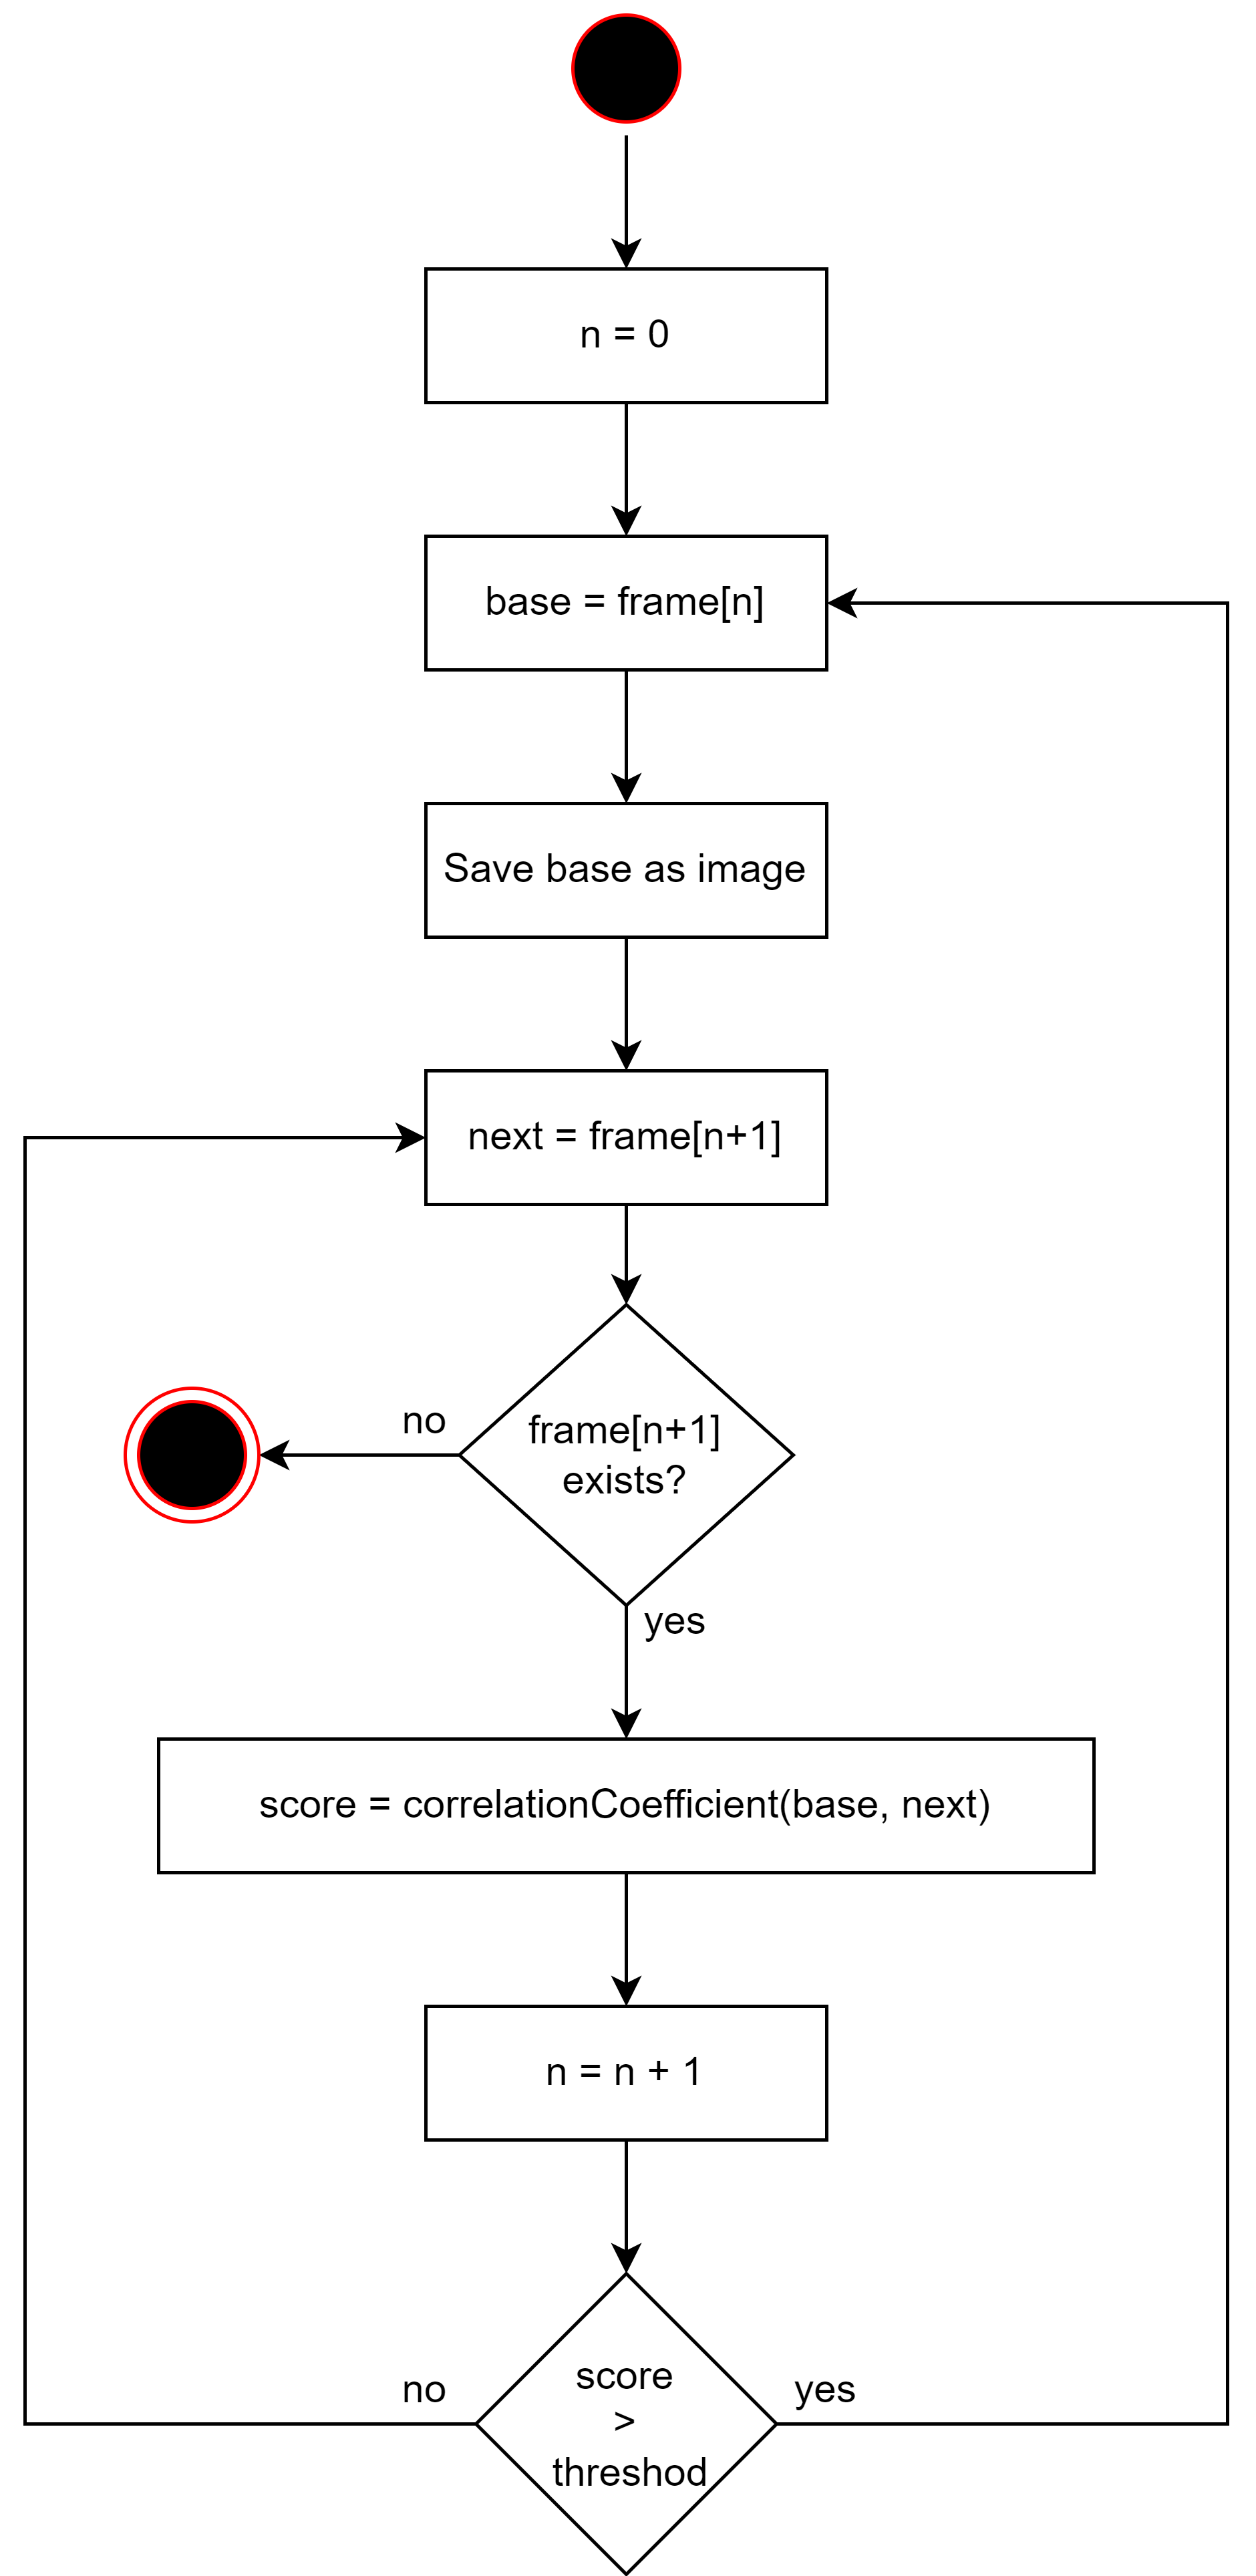
\includegraphics[width=0.5\textwidth]{diagrams/FlowChart-VideoToFrames.png}
    \caption{Video to frames flowchart}
    \end{figure}
% ================================================================================================= 
        \subsection{Data Preparation}
            During the collection of images to use for the dataset, certain classes had much more samples to choose from compared to others, which led to an imbalanced problem.
            Predictive modeling is challenged by imbalanced classifications since the majority of machine learning methods for classification were built on the premise that there should be an equal number of samples in each class. This is because most algorithms are intended to be as accurate and error-free as possible.
            However, if the data set is imbalanced, the model may still forecast the majority class with a high degree of accuracy but not the minority class, which is often the goal of the model in the first place.
            \subsubsection{Split Dataset}
    A customized under-sampling technique was used to avoid this situation. 
    The standard under-sampling technique does not meet the requirement simply due to the fact that many of the images used for the dataset have multiple labels.
    In other words, elimination of an image will lead to the perishment of many other labels.
    \paragraph{Calculating Quantity}
        Firstly, start with finding the lowest number of labels out of all the classes to set a standard upon which to divide a ratio between training, validating, and testing. The sum of the ratio of each dataset must be equal to 1:\\
        \begin{center}
            \(p(train) + p(val) + p(test) = 1\) 
        \end{center} 
        From that, calculate the number of labels per class needed in each subset by:
        \begin{center}
            \(n(train) = p(train) * standard\) \\
            \(n(val) = p(val) * standard\) \\
            \(n(test) = p(test) * standard\) 
        \end{center} 
    \paragraph{Customized Under-sampling Algorithm}
        The choose approach was employed as opposed to deleting. 
        The algorithm will first loop over all of the classes that are available. 
        After that, sort the dataset by how many labels there are in total for that class for each image. 
        The image will be chosen by an algorithm from left to right. 
        The image will be added to the new dataset if the total number of labels from each class does not exceed the predetermined number in the previous section (\autoref{fig:CustomizedUnderSampling}).
            \subsubsection{Data Augmentation}
    Generally, when using Machine Learning for classification problems, it is more ideal to learn a classifier that can perform well on a population. 
    An example of a population would be the set of all handwritten characters in the entire world. Generally, that complete population will not always be available for training, we only have a much smaller training dataset. 
    If a training set is large enough, it might be a good approximation of the population we're interested in, but it's still just that, an approximation.
    
    A learning algorithm is over-fitting if it performs significantly better on the training set than it is on the population (which will be generally approximated again using a separate test set).
    
    To help combat over-fitting and data deficiency, along with increasing the model's accuracy, Data Augmentation techniques are used to diversify existing data points.
    Data augmentation is an effective method for enhancing the performance of our computer vision models without having to collect more data.
    \label{Figure Data Augmentation}
\begin{figure}[H]
    \centering
    \begin{subfigure}{0.15\textwidth}
        \centering
        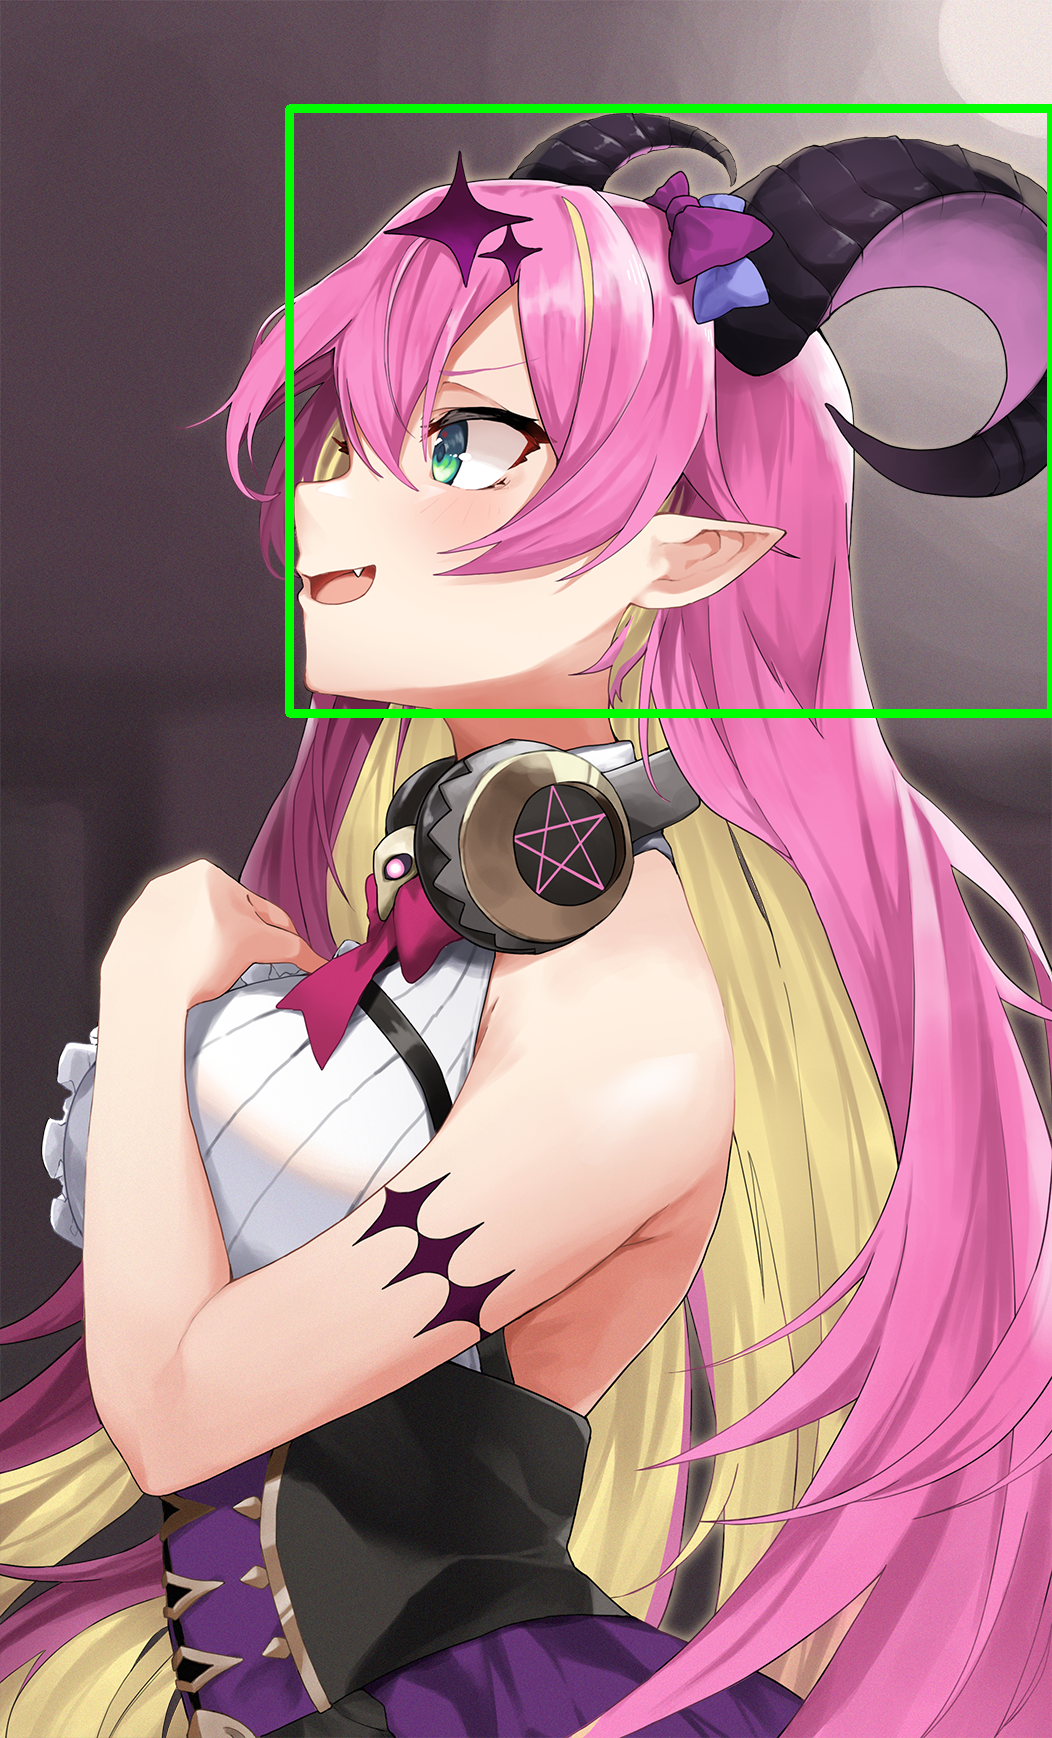
\includegraphics[width=\textwidth]{images/augmentation/Pixiv-83768702_p0-BB.png}
        \caption{}
        \label{fig:aloe1}
    \end{subfigure}
    \hfill
    \begin{subfigure}{0.15\textwidth}
        \centering
        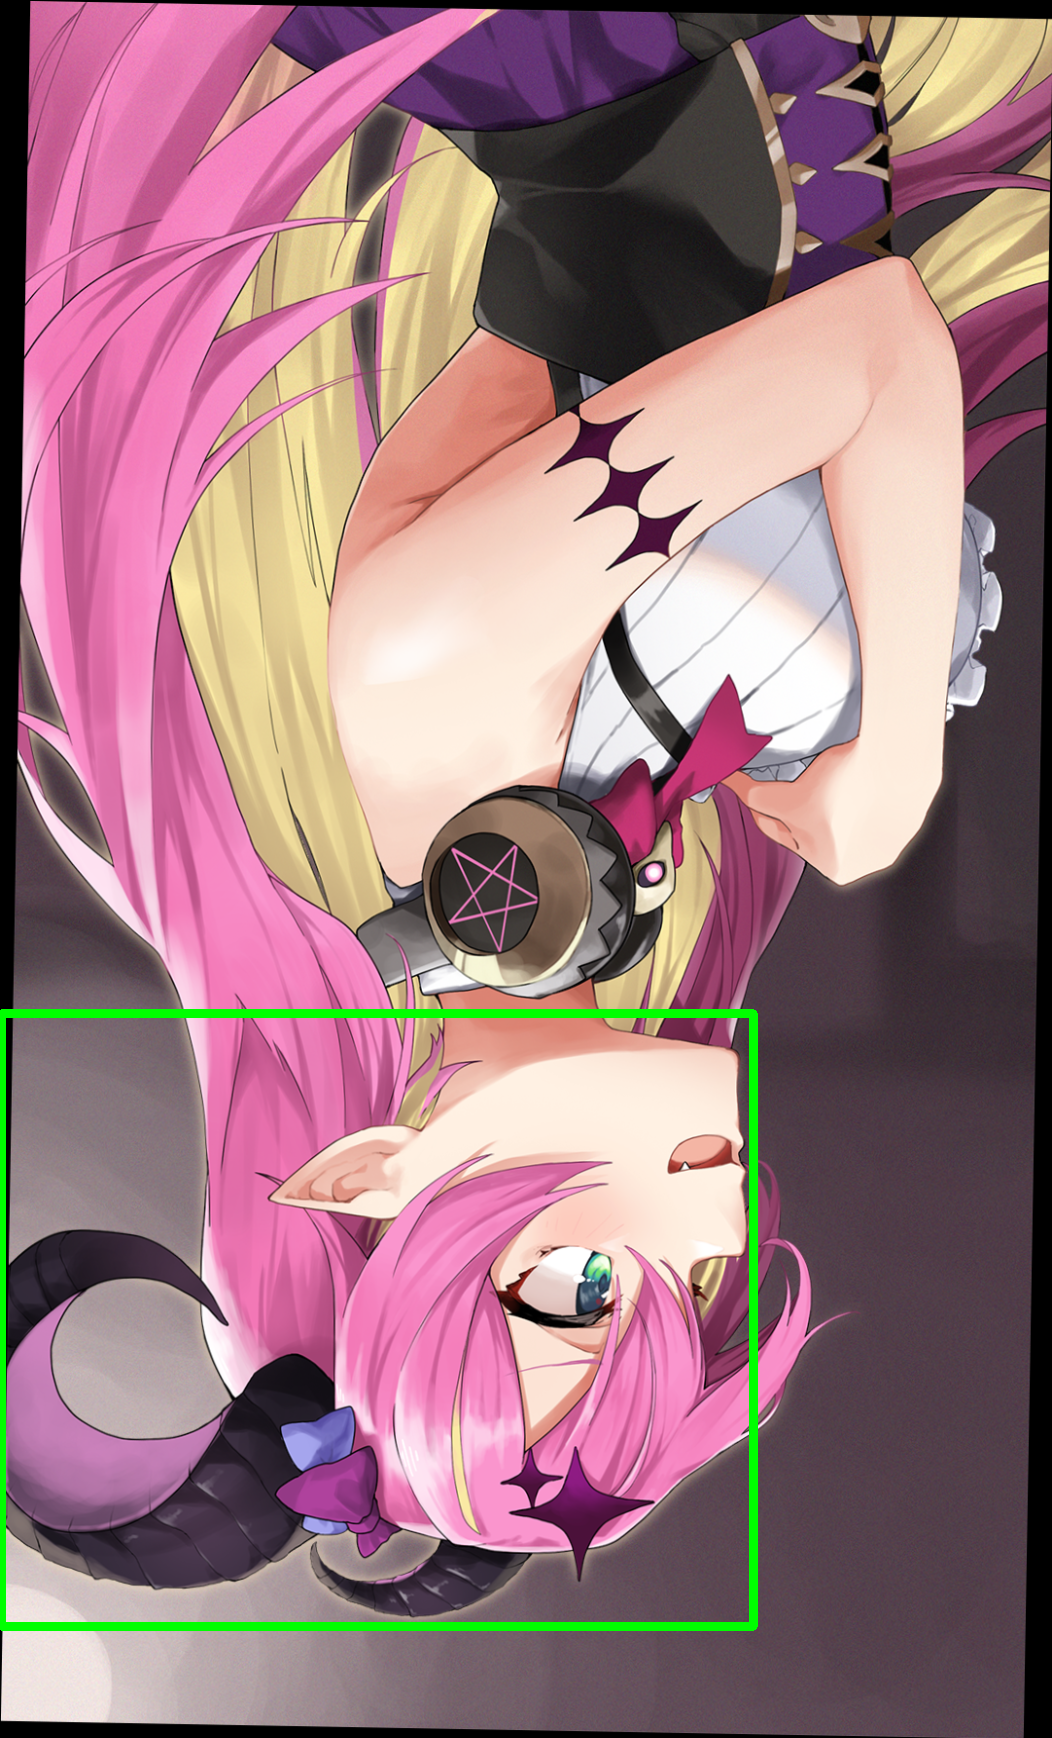
\includegraphics[width=\textwidth]{images/augmentation/Pixiv-83768702_p0-RandomRotate_179-BB.png}
        \caption{}
        \label{fig:aloe2}
    \end{subfigure}
    \hfill
    \begin{subfigure}{0.15\textwidth}
        \centering
        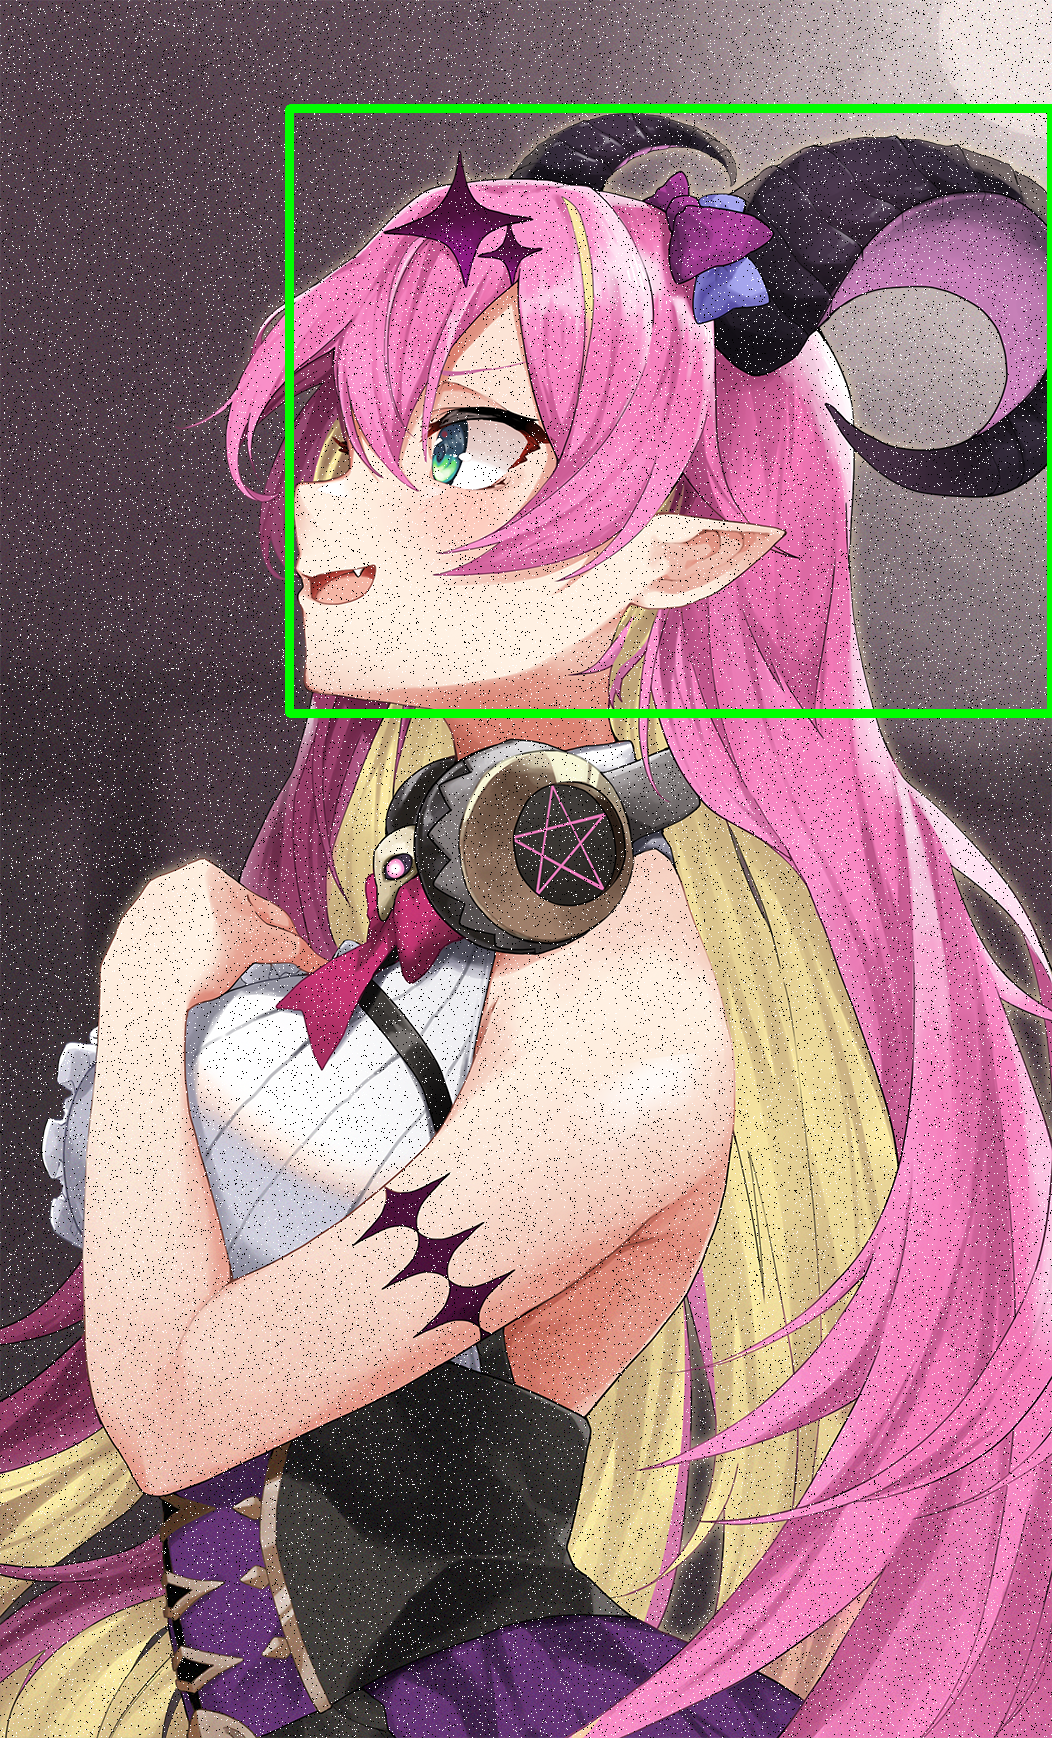
\includegraphics[width=\textwidth]{images/augmentation/Pixiv-83768702_p0-RandomSaltAndPepper_0.044-BB.png}
        \caption{}
        \label{fig:aloe3}
    \end{subfigure}
    \hfill
    \begin{subfigure}{0.15\textwidth}
        \centering
        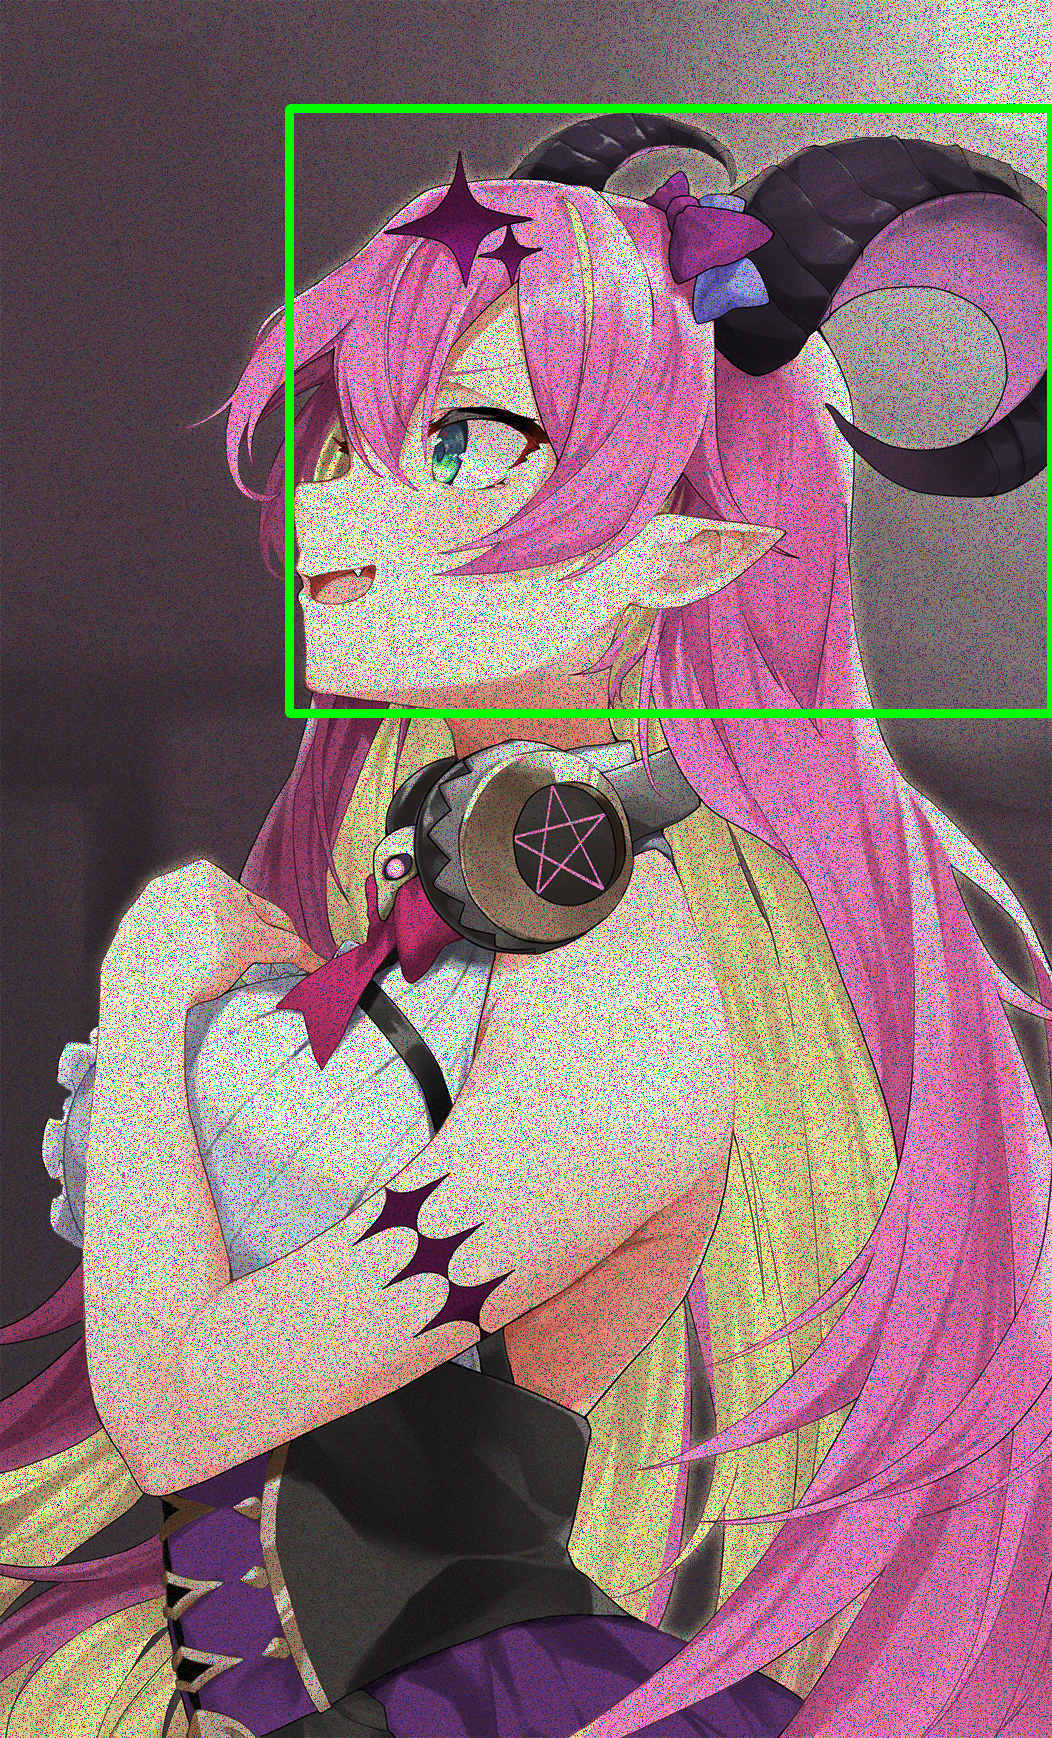
\includegraphics[width=\textwidth]{images/augmentation/Pixiv-83768702_p0-RandomValuedImpulseNoise_0.138-BB.png}
        \caption{}
        \label{fig:aloe4}
    \end{subfigure}
    \begin{subfigure}{0.15\textwidth}
        \centering
        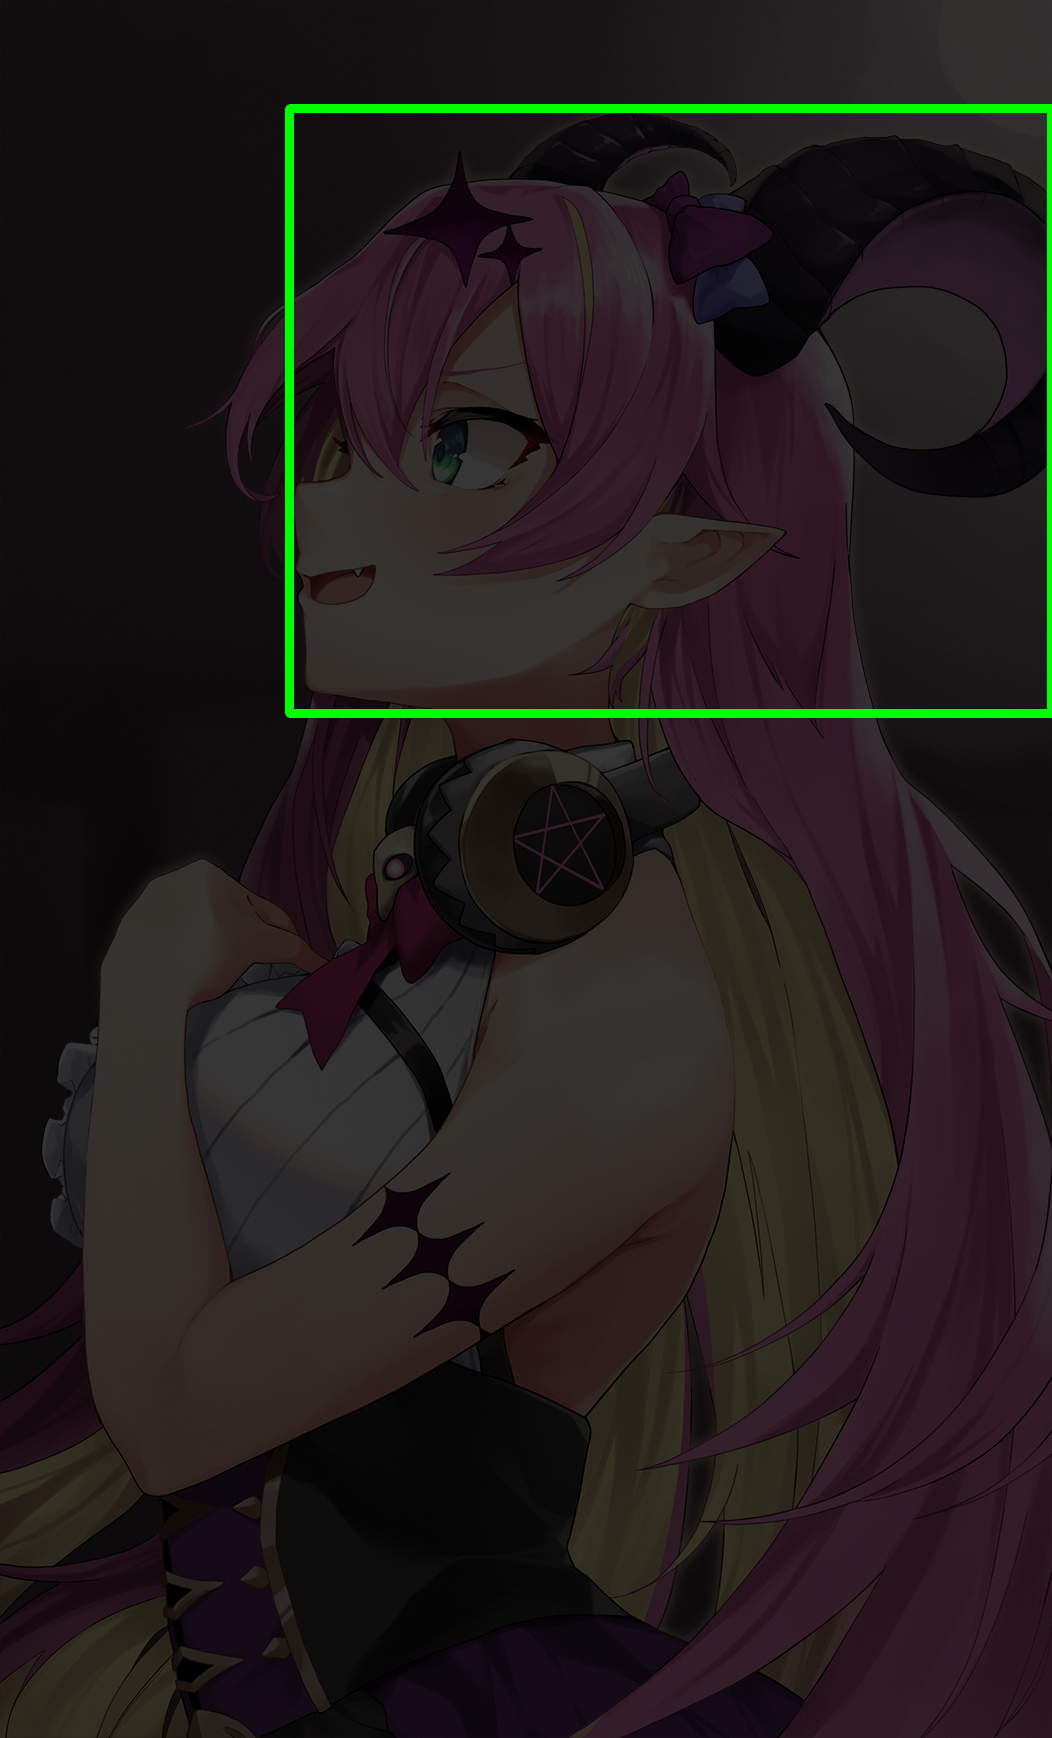
\includegraphics[width=\textwidth]{images/augmentation/Pixiv-83768702_p0-RandomBrightness_0.213-BB.png}
        \caption{}
        \label{fig:aloe5}
    \end{subfigure}
    \begin{flushleft}
        (a) Original image\cite{83768702}\\
        (b) Rotate 179 degrees\\
        (c) Random Salt and Pepper with 4.4\% \\
        (d) Random Valued Impulse Noise with 13.8\% \\
        (e) Brightness with intensity 0.213\\
    \end{flushleft}
    \caption{Data augmentation methods}
    \label{fig:manoaloe1}
\end{figure}
    \paragraph{Random-valued Impulse Noise, Salt and Pepper}
        Real-world data is seldom clean. At least it is not as clean as the data that we train our model on. 
        Noise in the data can reduce the accuracy of the model and lead to less generalization power. 
        This is the main reason why many times deep neural network models perform poorly during testing. 
        Therefore, noise are used to augment data. Not only will there be more data to use for training, 
        but the noisy data used for training the model will also make it better at generalizing real-world noisy data.
        \begin{lstlisting}[language=Python]
mask = np.random.rand(*self.image.shape[:2])
mask = np.concatenate([mask, mask, mask])
mask = mask.reshape(*mask.shape, 3)
self.image = np.where(
                self.portion*2>mask,
                np.random.randint(low=0, 
                                  high=255, 
                                  size=1, 
                                  dtype=int),
                self.image) 
        \end{lstlisting}
% =========================================================
    \paragraph{Random Brightness}
         Training the model with images with various luminosity will help it better generalize images that are not trained even on different lighting conditions\cite{RandomBrightness}. 
         The brightness and darkness depend upon one boundary value which is 1.0.
         At 1.0, the image will be in its original state.
         If the value is less than 1.0 then it will darken the image like [0.1,1.0), whereas a value greater than 1.0 makes the image brighter like (1.0, 2.0].
         At level 0 of luminosity, the image is filled with black pixels.
         \begin{lstlisting}[language=Python]
img = (self.image * self.level).astype(int)
self.image = np.clip(a=img,
                     a_min=0,
                     a_max=255)
         \end{lstlisting}
% =========================================================
    \paragraph{Image rotation}
        \label{Figure Rotation Formula}
\begin{figure}[H]
    \centering
    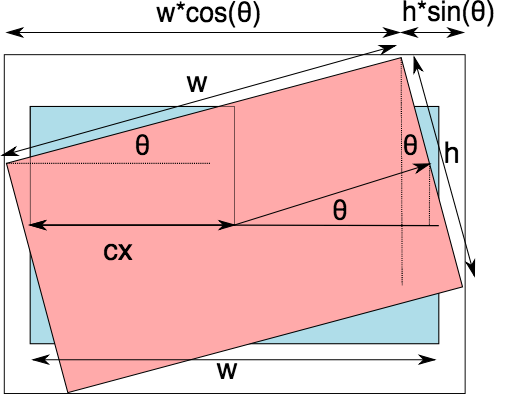
\includegraphics[width=0.4\textwidth]{Picture2.png}
    \label{fig:pic2}
    \begin{center}
        \begin{align*}
            N_{w} = h * \sin(\theta) + w * \cos(\theta)\\
            N_{h} = h * \cos(\theta) + w * \sin(\theta)
        \end{align*}
    \end{center}
    \caption{Rotation Formula}
\end{figure}
        \label{Figure Image Rotation}
\begin{figure}[H]
    \centering
    \begin{subfigure}{0.15\textwidth}
        \centering
        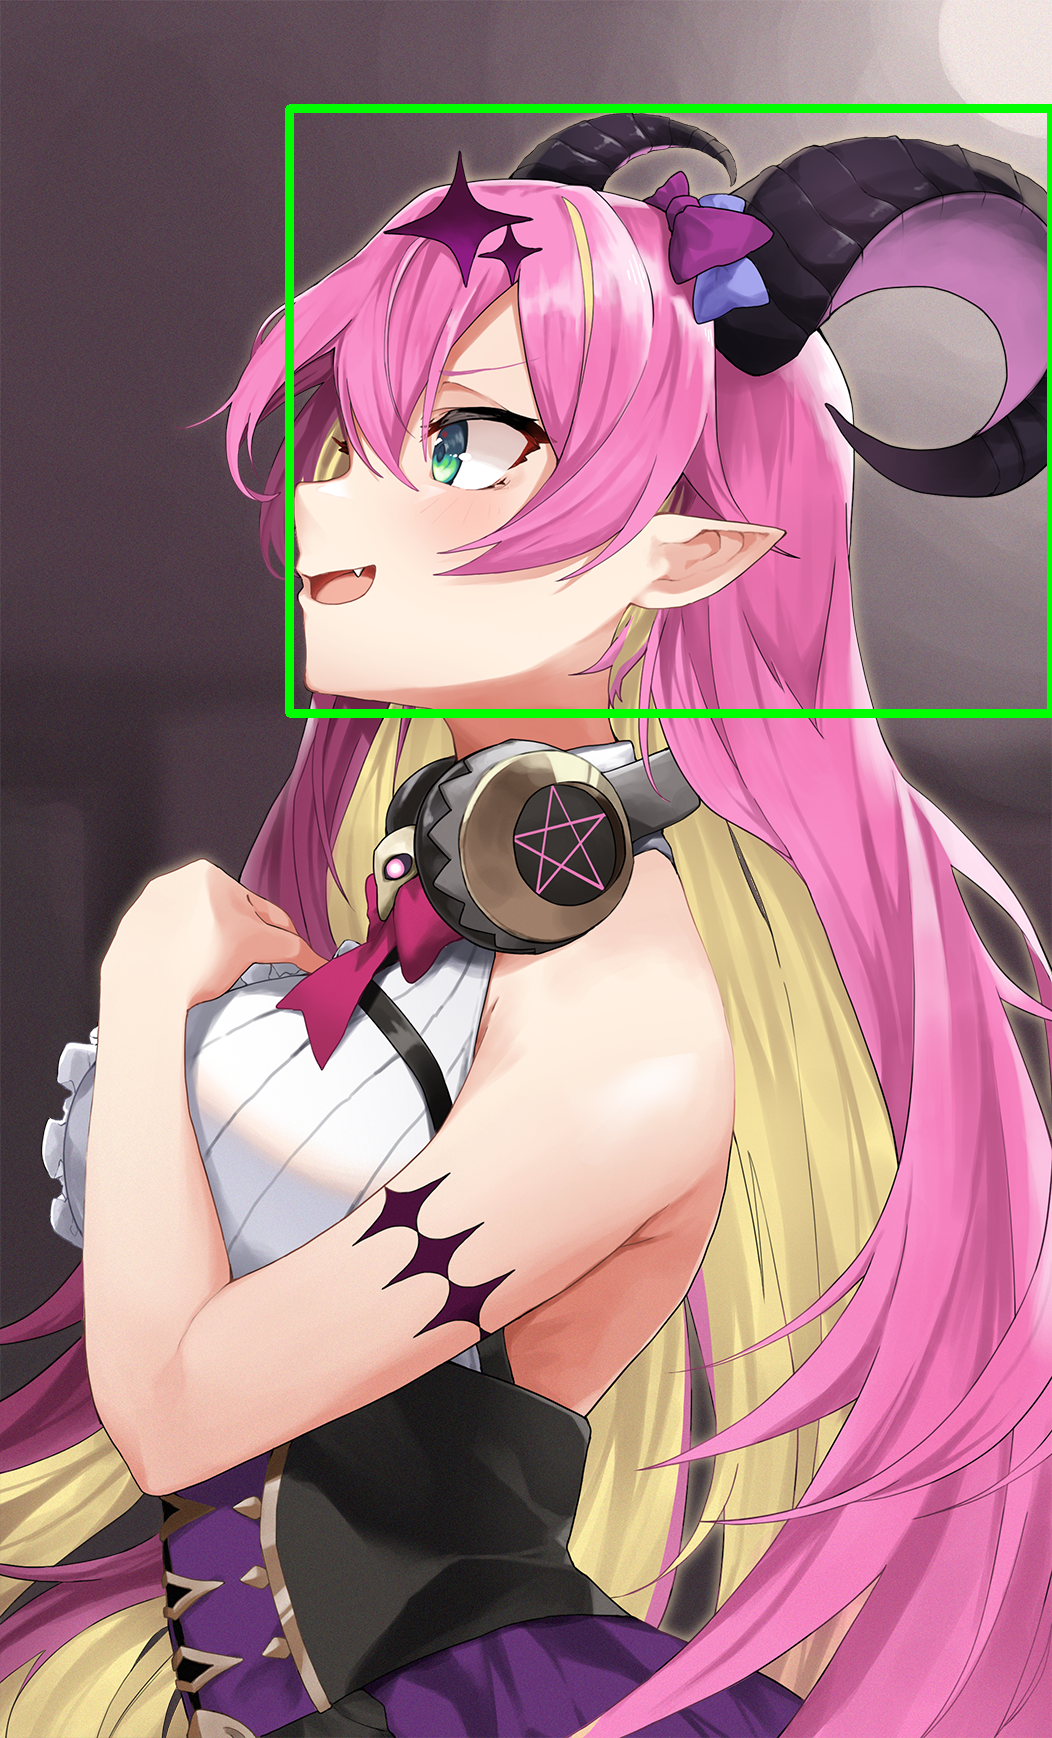
\includegraphics[width=\textwidth]{images/augmentation/Pixiv-83768702_p0-BB.png}
        % \caption{Original}
        \caption{}
        \label{fig:aloe1}
    \end{subfigure}
    \hfill
    \begin{subfigure}{0.15\textwidth}
        \centering
        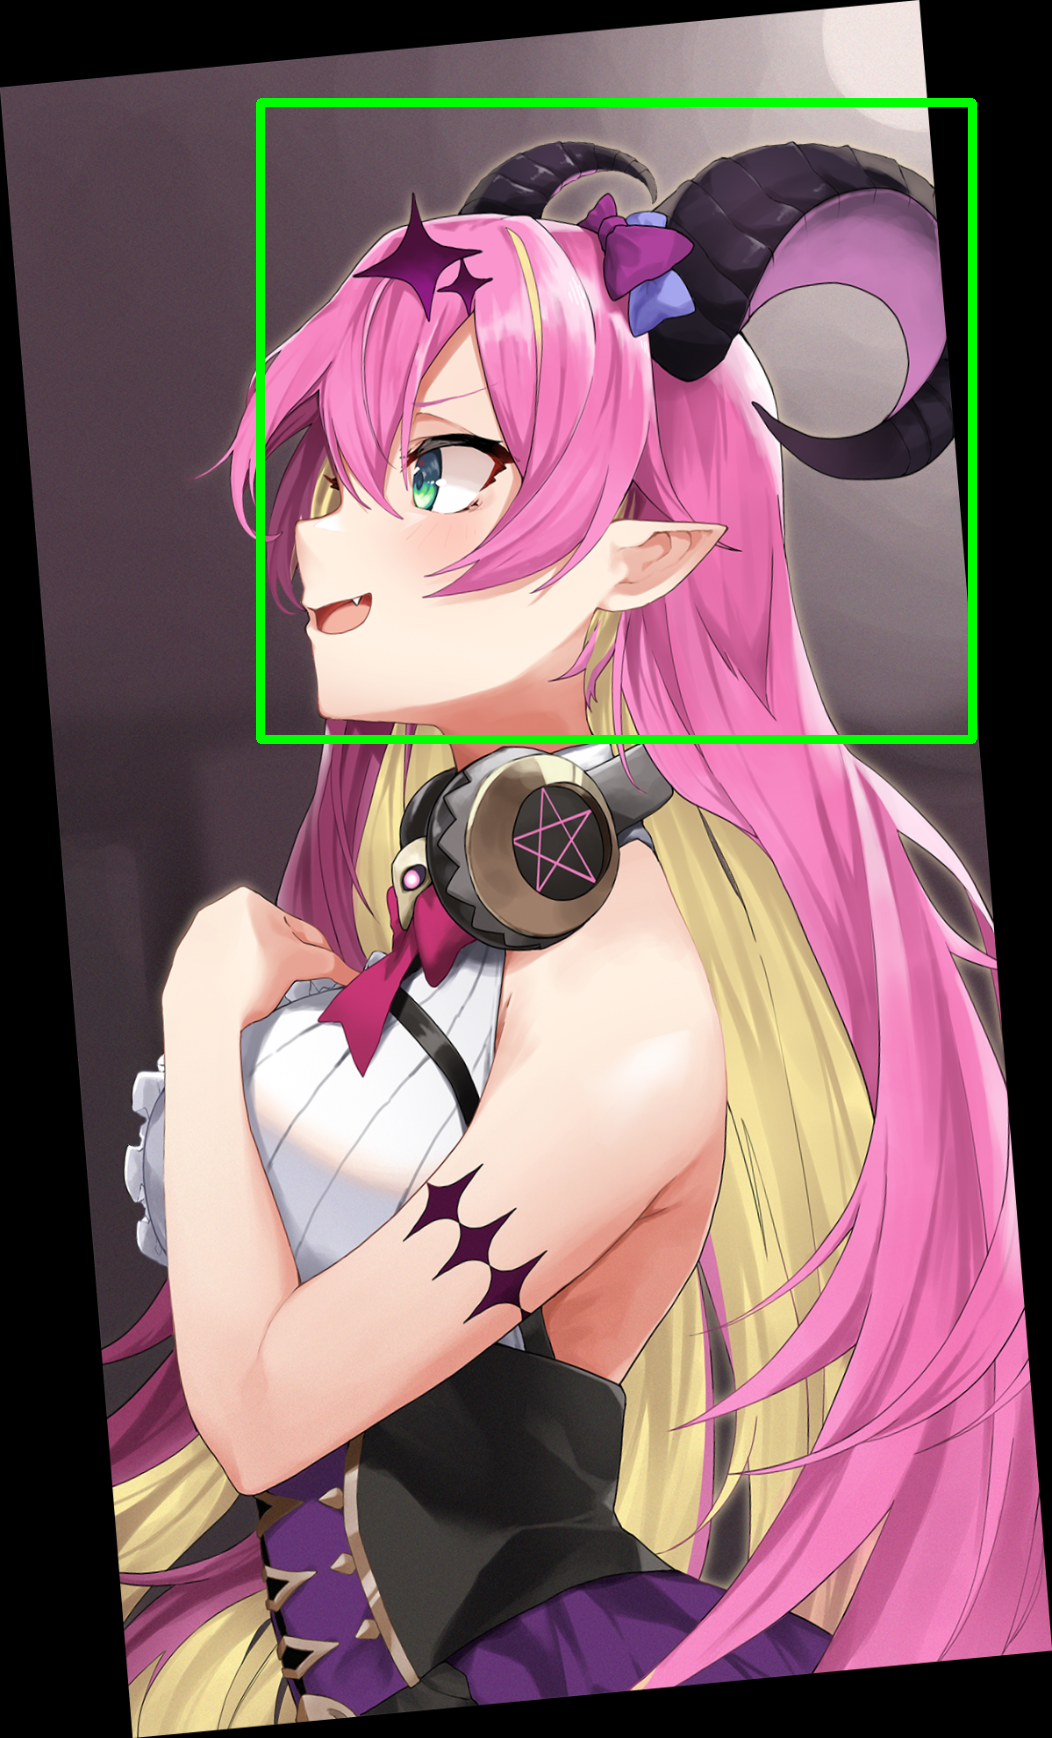
\includegraphics[width=\textwidth]{images/augmentation/Pixiv-83768702_p0-RandomRotate_5-BB.png}
        % \caption{5 degrees}
        \caption{}
        \label{fig:aloe2}
    \end{subfigure}
    \hfill
    \begin{subfigure}{0.15\textwidth}
        \centering
        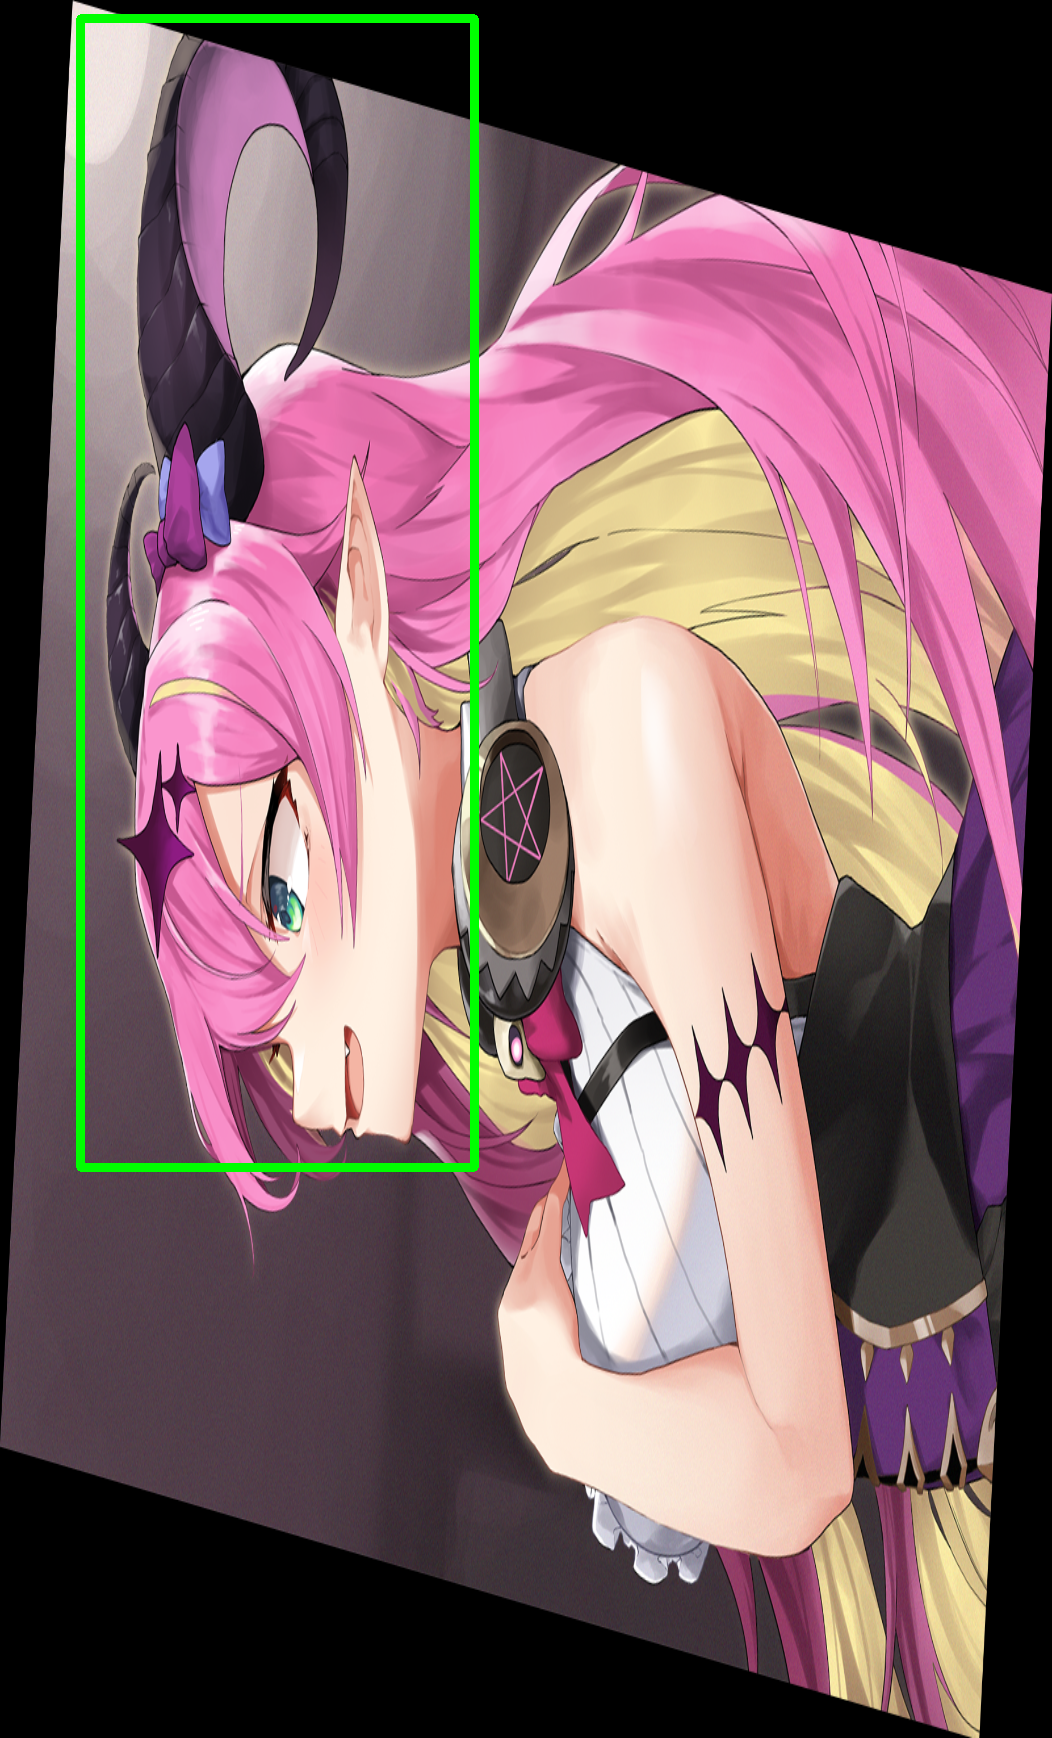
\includegraphics[width=\textwidth]{images/augmentation/Pixiv-83768702_p0-RandomRotate_83-BB.png}
        % \caption{83 degrees}
        \caption{}
        \label{fig:aloe3}
    \end{subfigure}
    \hfill
    \begin{subfigure}{0.15\textwidth}
        \centering
        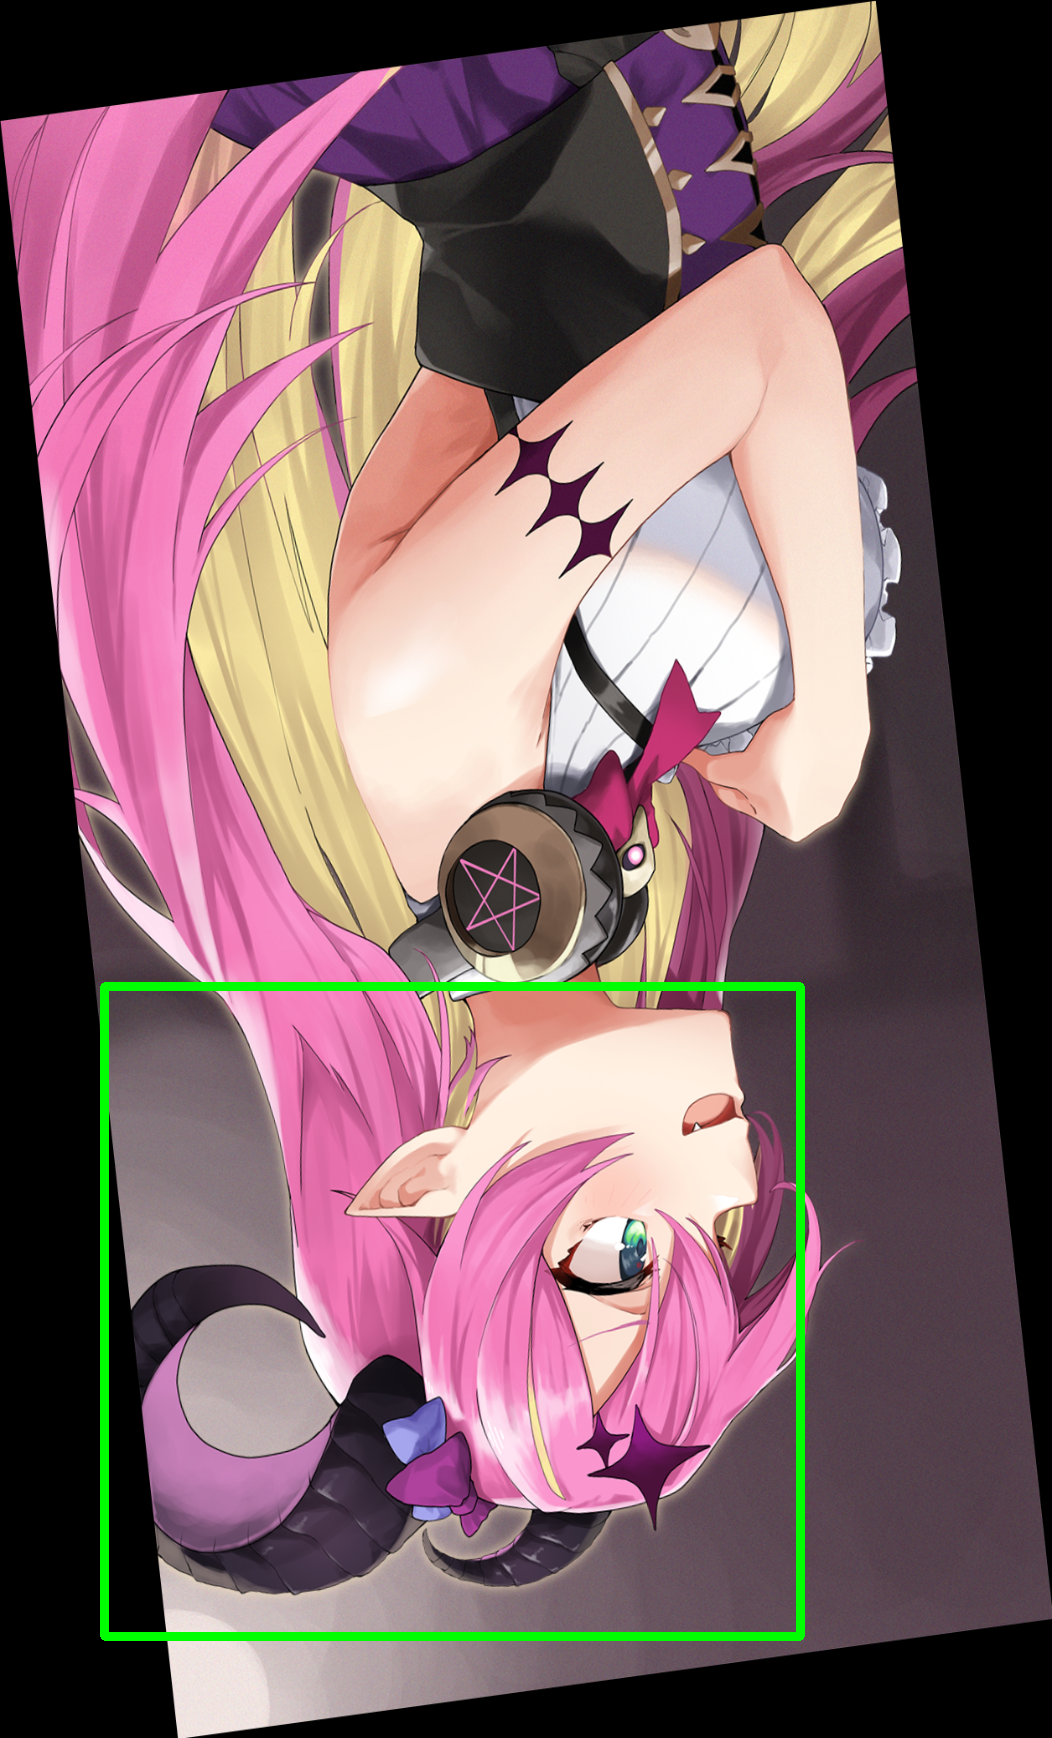
\includegraphics[width=\textwidth]{images/augmentation/Pixiv-83768702_p0-RandomRotate_187-BB.png}
        % \caption{187 degrees}
        \caption{}
        \label{fig:aloe4}
    \end{subfigure}
    \begin{subfigure}{0.15\textwidth}
        \centering
        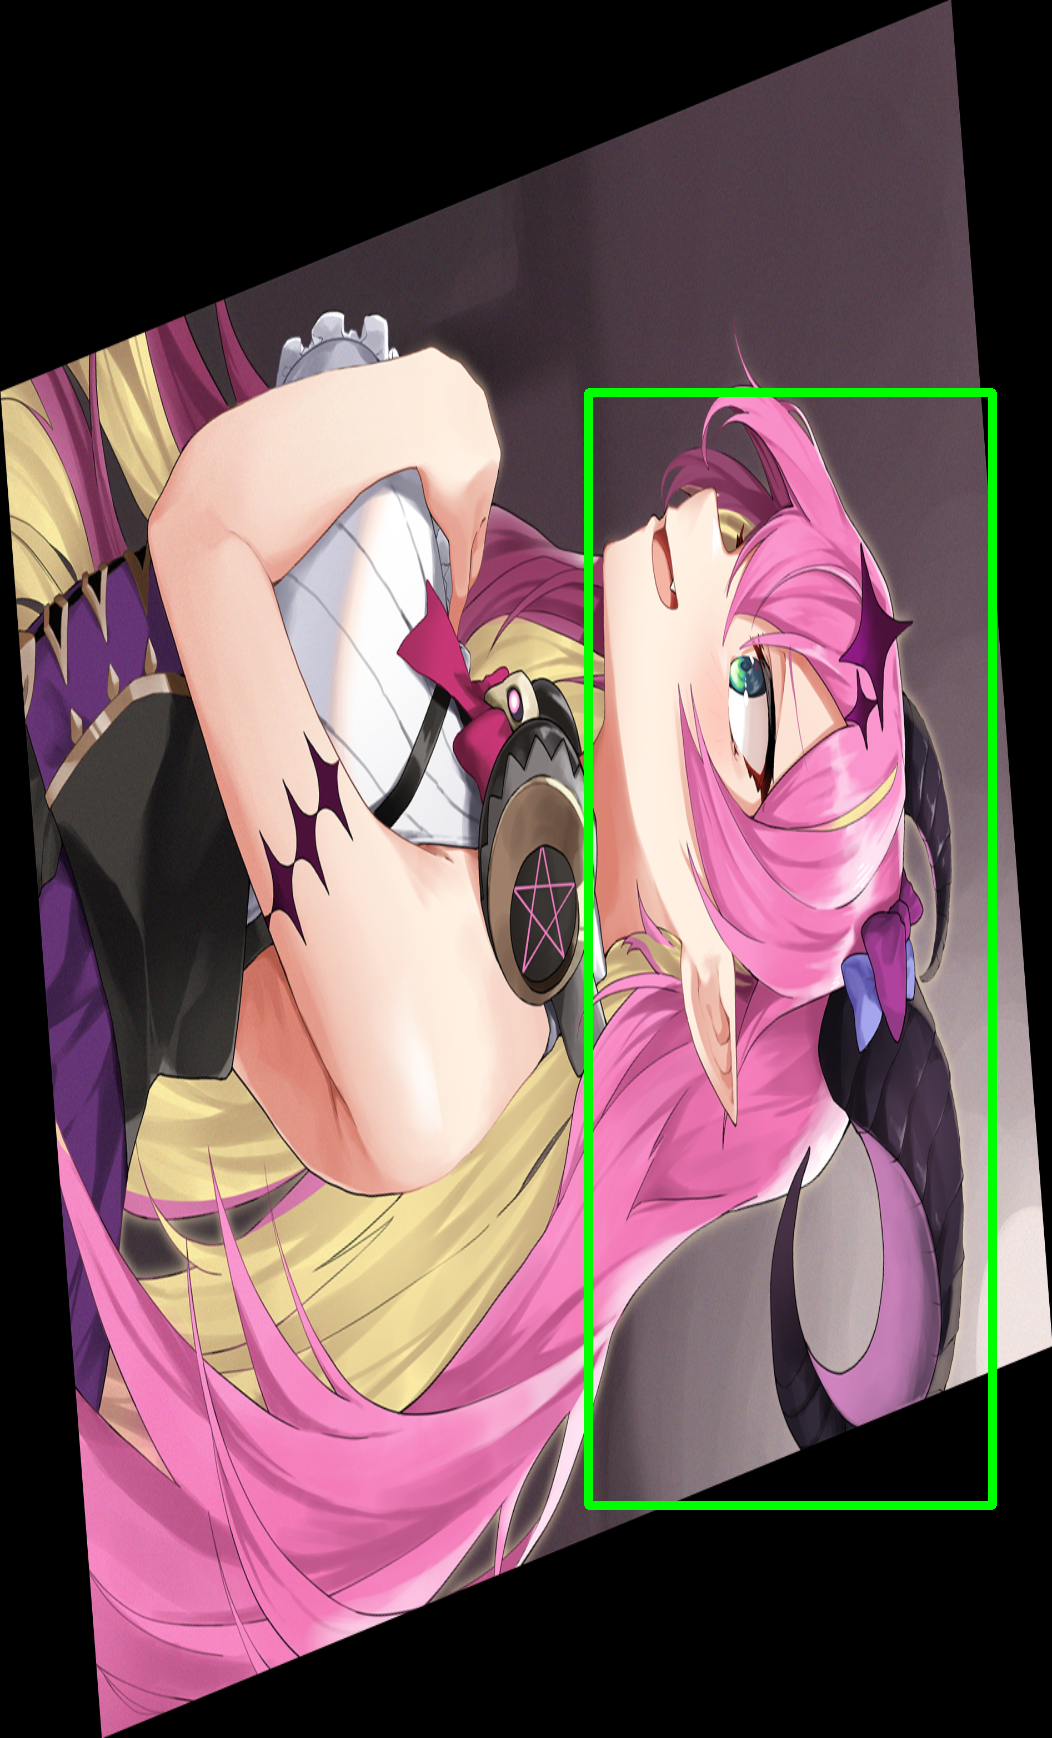
\includegraphics[width=\textwidth]{images/augmentation/Pixiv-83768702_p0-RandomRotate_280-BB.png}
        % \caption{280 degrees}
        \caption{}
        \label{fig:aloe5}
    \end{subfigure}
    \begin{flushleft}
        (a) Original image\cite{83768702}\\
        (b) Rotate with 5 degrees\\
        (c) Rotate with 83 degrees\\
        (d) Rotate with 187 degrees\\
        (e) Rotate with 280 degrees\\
    \end{flushleft}
    \caption{Image Rotation}
    \label{fig:manoaloe1}
\end{figure}
        Because it alters the angles at which objects appear in the dataset during training, Random Rotate is a particularly helpful augmentation. 
        Perhaps images were only taken with an item horizontally throughout the image gathering phase, but the object could have been skewed in any direction during manufacturing. 
        However, this method is by far the most sophisticated. 
        The items in an image are also relocated when it is rotated.
        However fortunately, we discovered a tutorial by Ayoosh Kathuria that can assist us in solving this issue with just some modification\cite{Rotation}.          
            \subsubsection{Adding Backgorund}
    Background images are those that do not have an object that needs to be classified to reduce False Positives (FP).
    Small chunks of background images are added to the training, validation, and testing datasets in addition to labeled images.
    As the background image fraction approaches 1.0, the training process will suffer.
    Background images should have a maximum proportion of 10 percent, as recommended by the author of YOLO5.
    In this project, background should be scenery images\cite{addingbackgroundimages}. 
    \begin{figure}[H]
    \centering
    \begin{subfigure}{0.241\textwidth}
        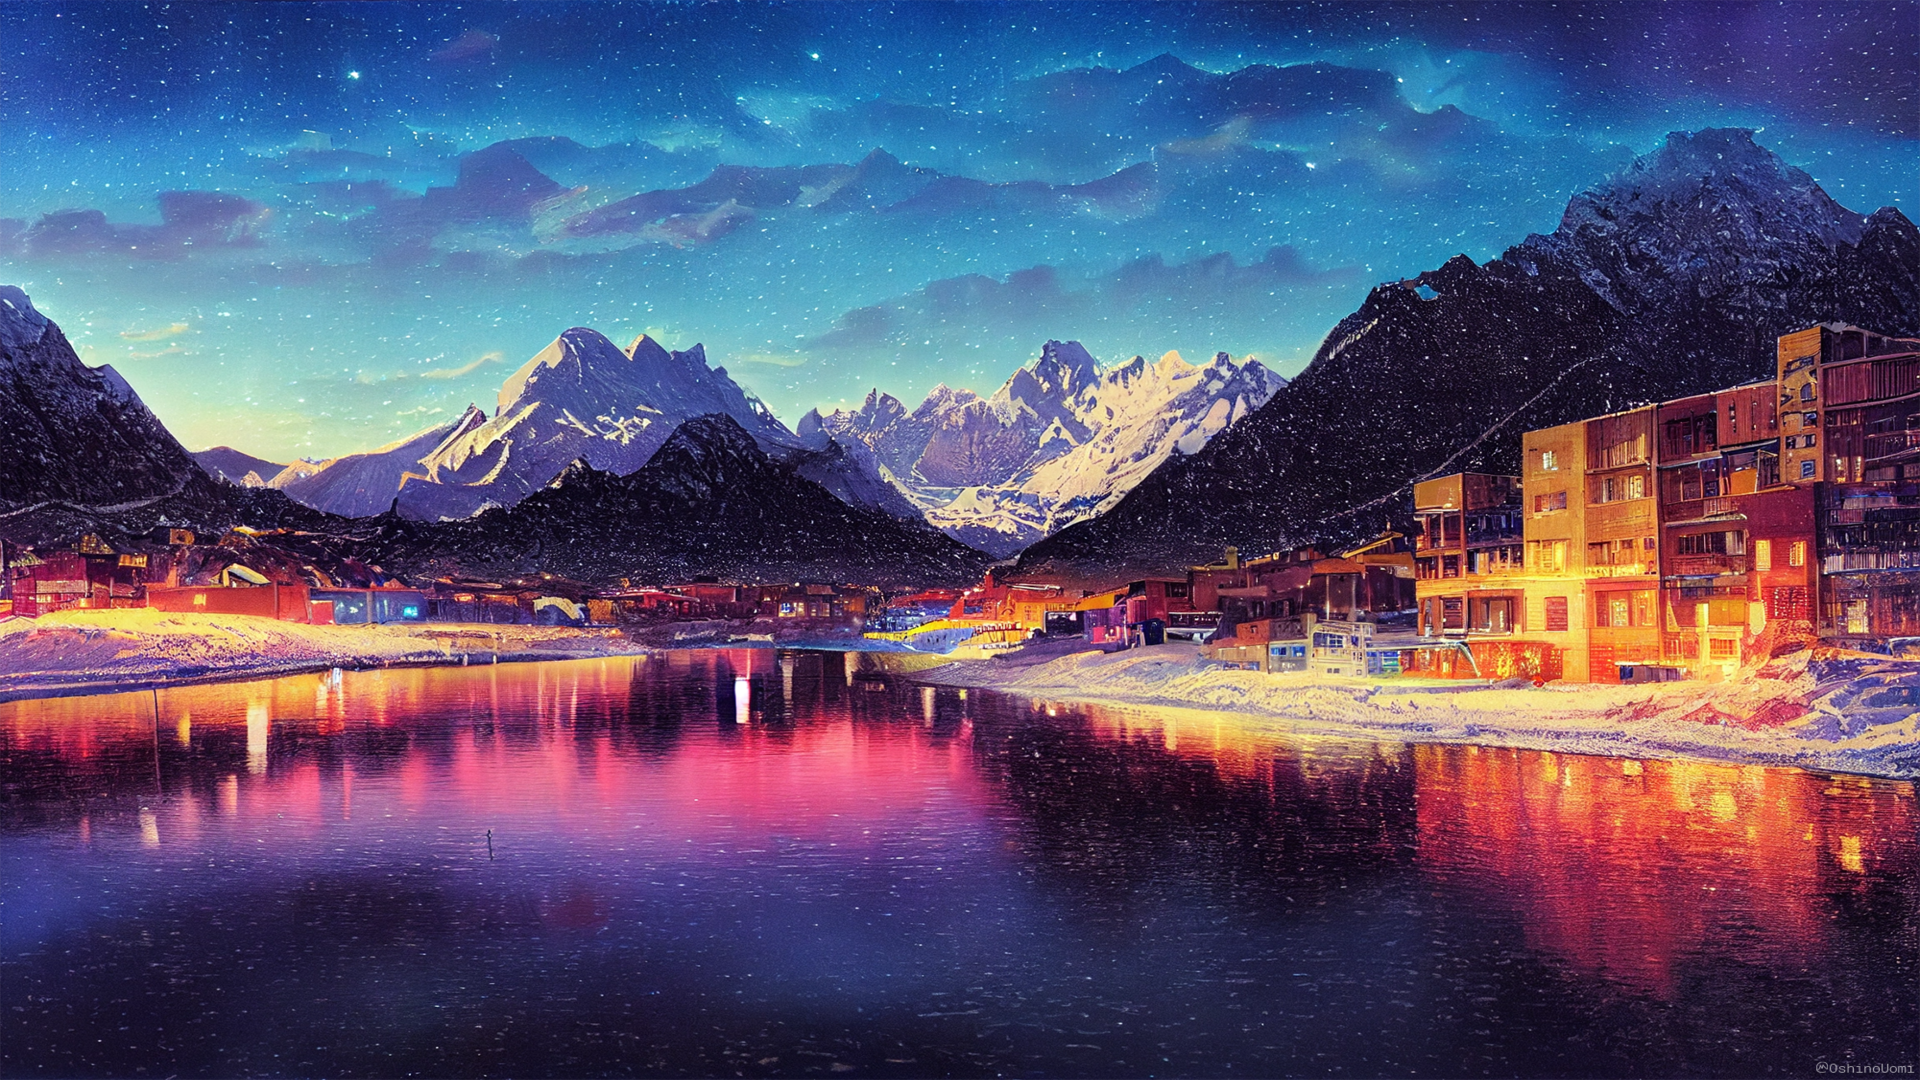
\includegraphics[width=1\textwidth]{images/background/Pixiv-101510980_p0.png}
    \end{subfigure}
    \hfill
    \begin{subfigure}{0.241\textwidth}
        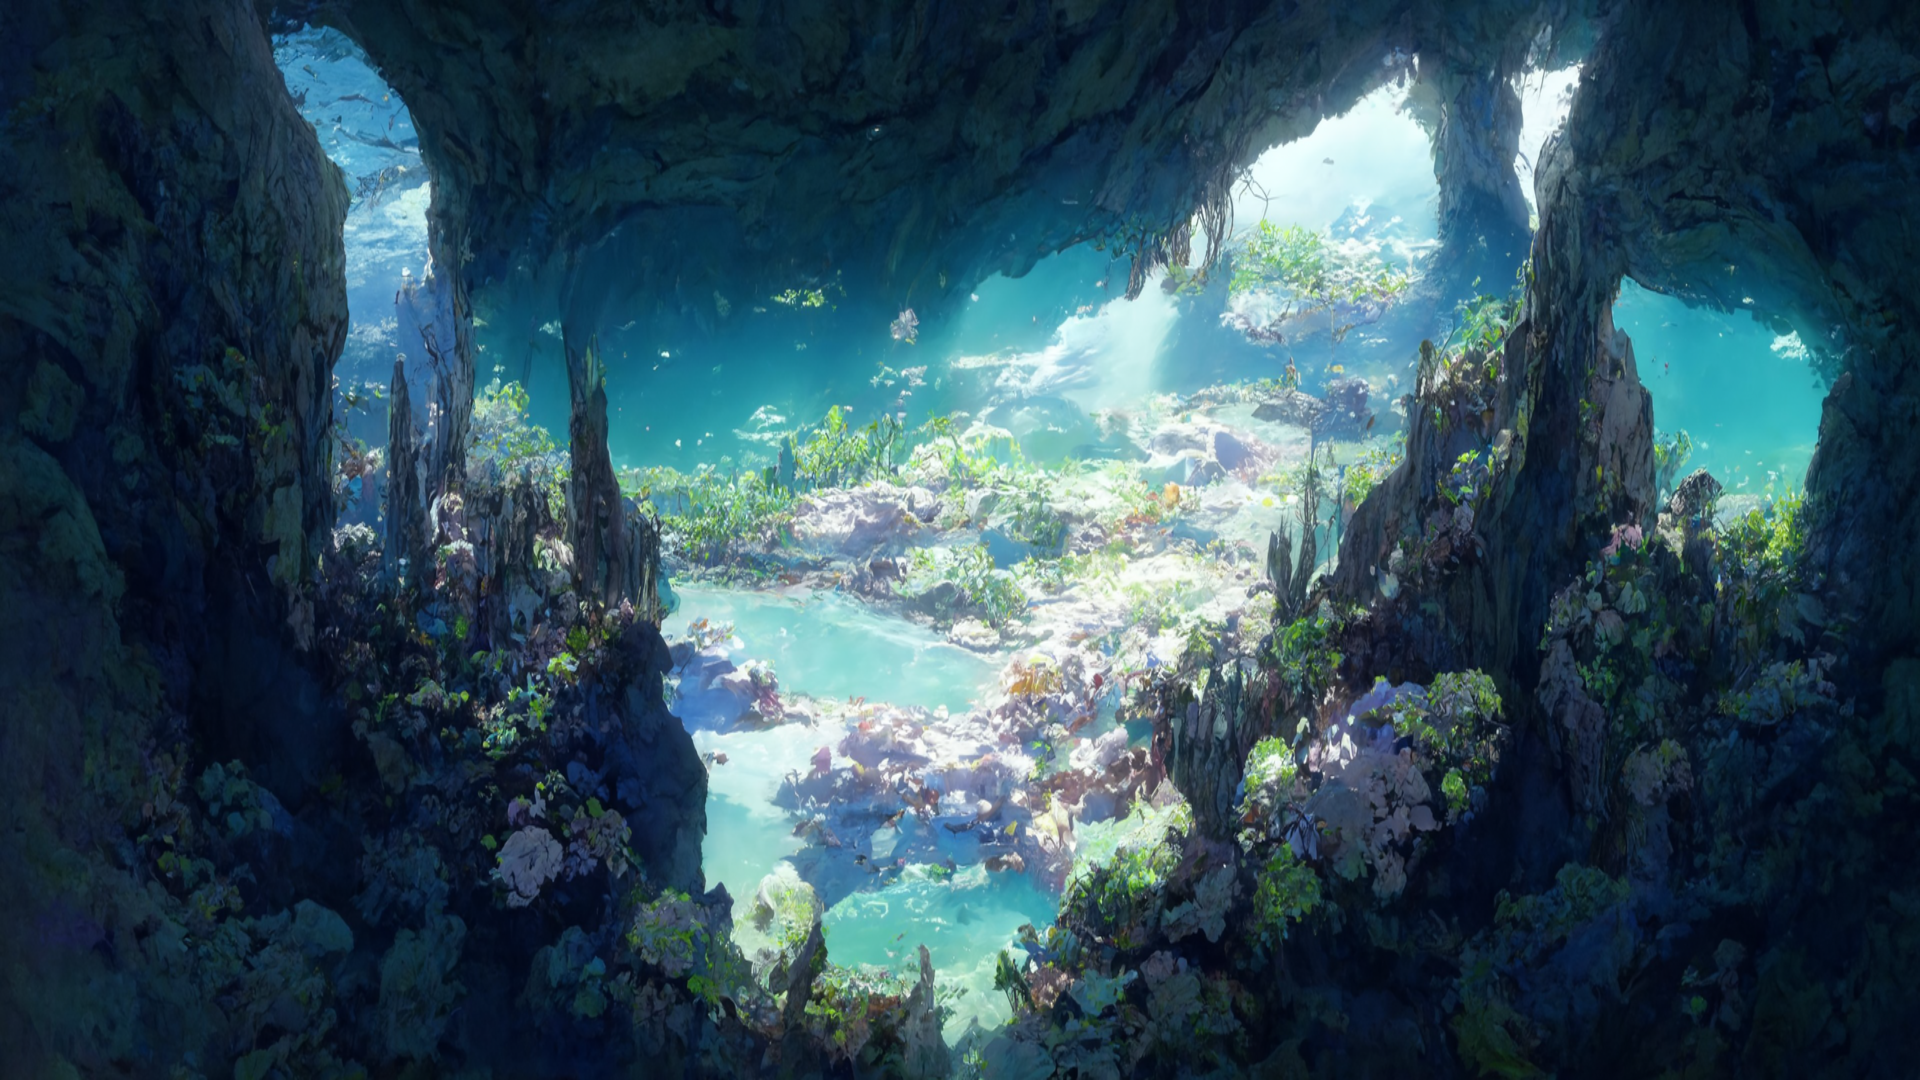
\includegraphics[width=1\textwidth]{images/background/Pixiv-100810147_p2.png}
    \end{subfigure}
    \hfill
    \begin{subfigure}{0.241\textwidth}
        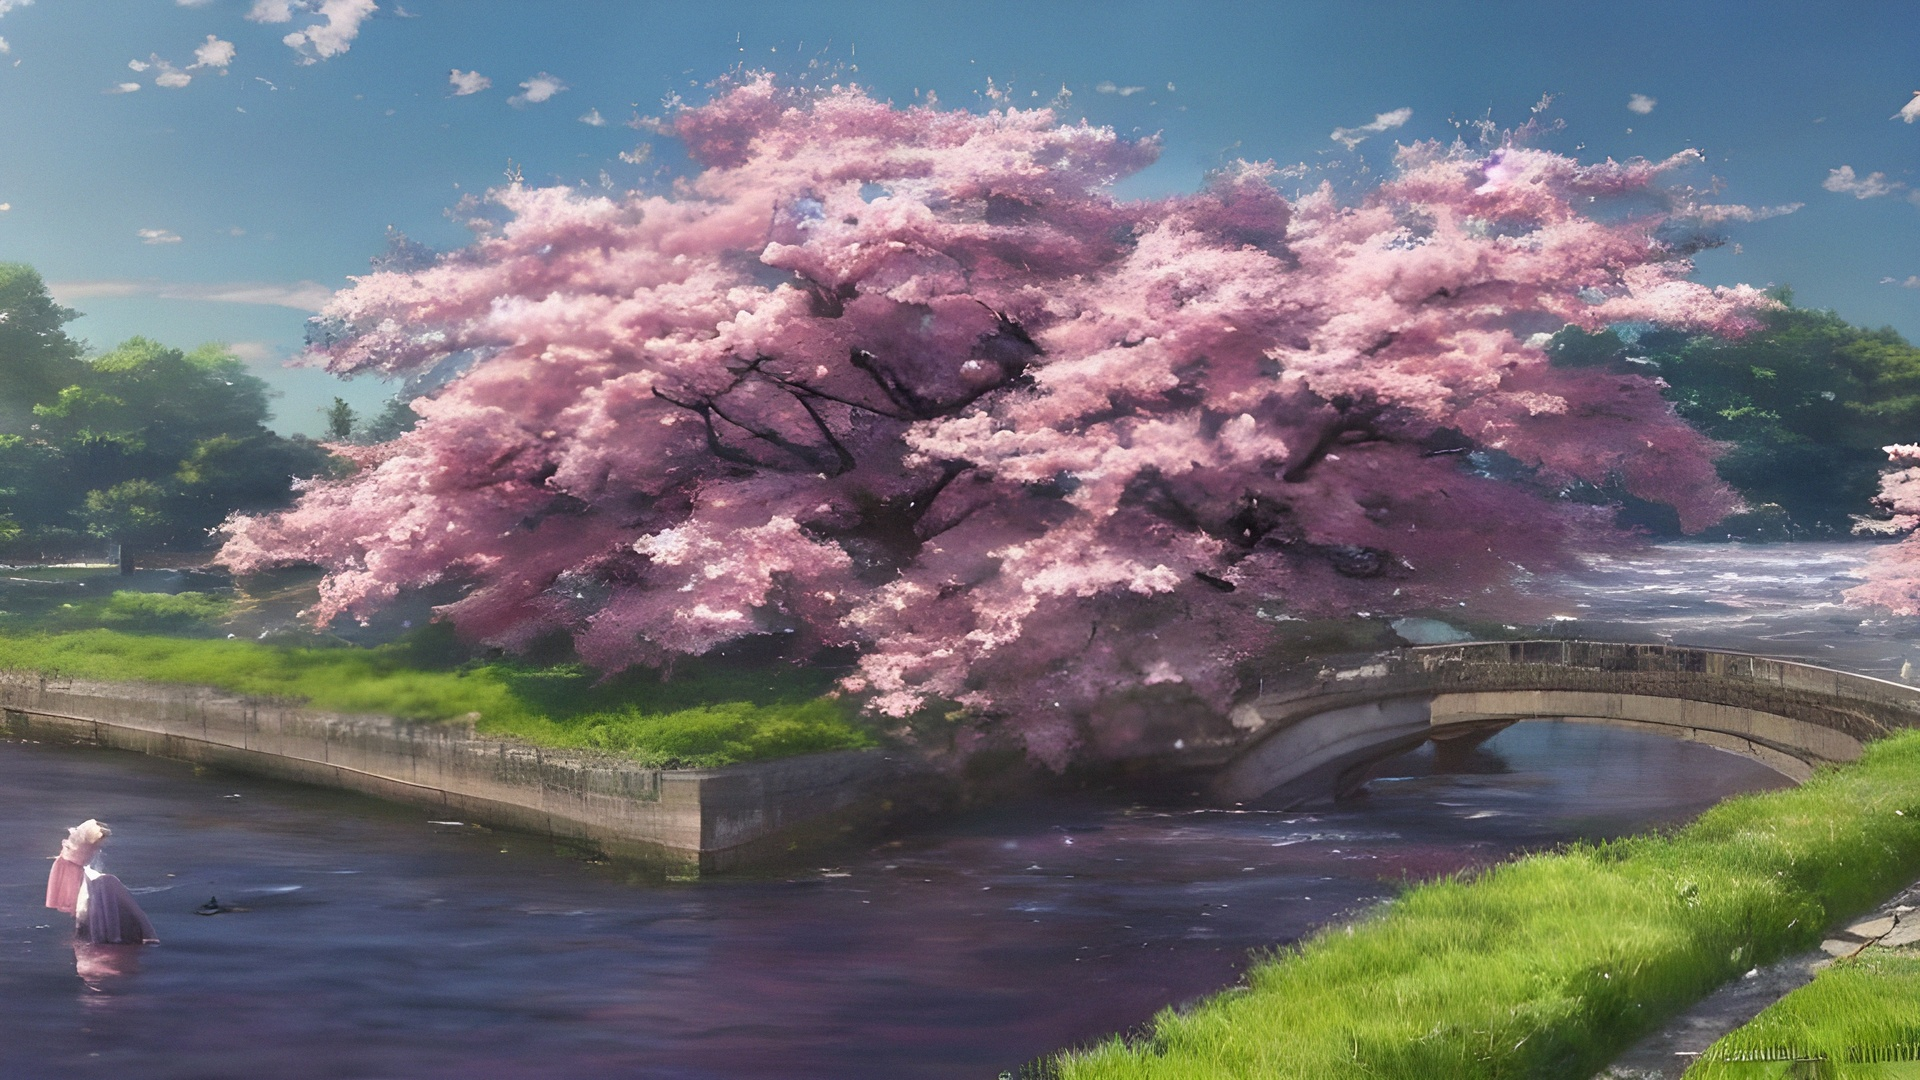
\includegraphics[width=1\textwidth]{images/background/Pixiv-101735564_p0.jpg}
    \end{subfigure}
    \hfill
    \begin{subfigure}{0.241\textwidth}
        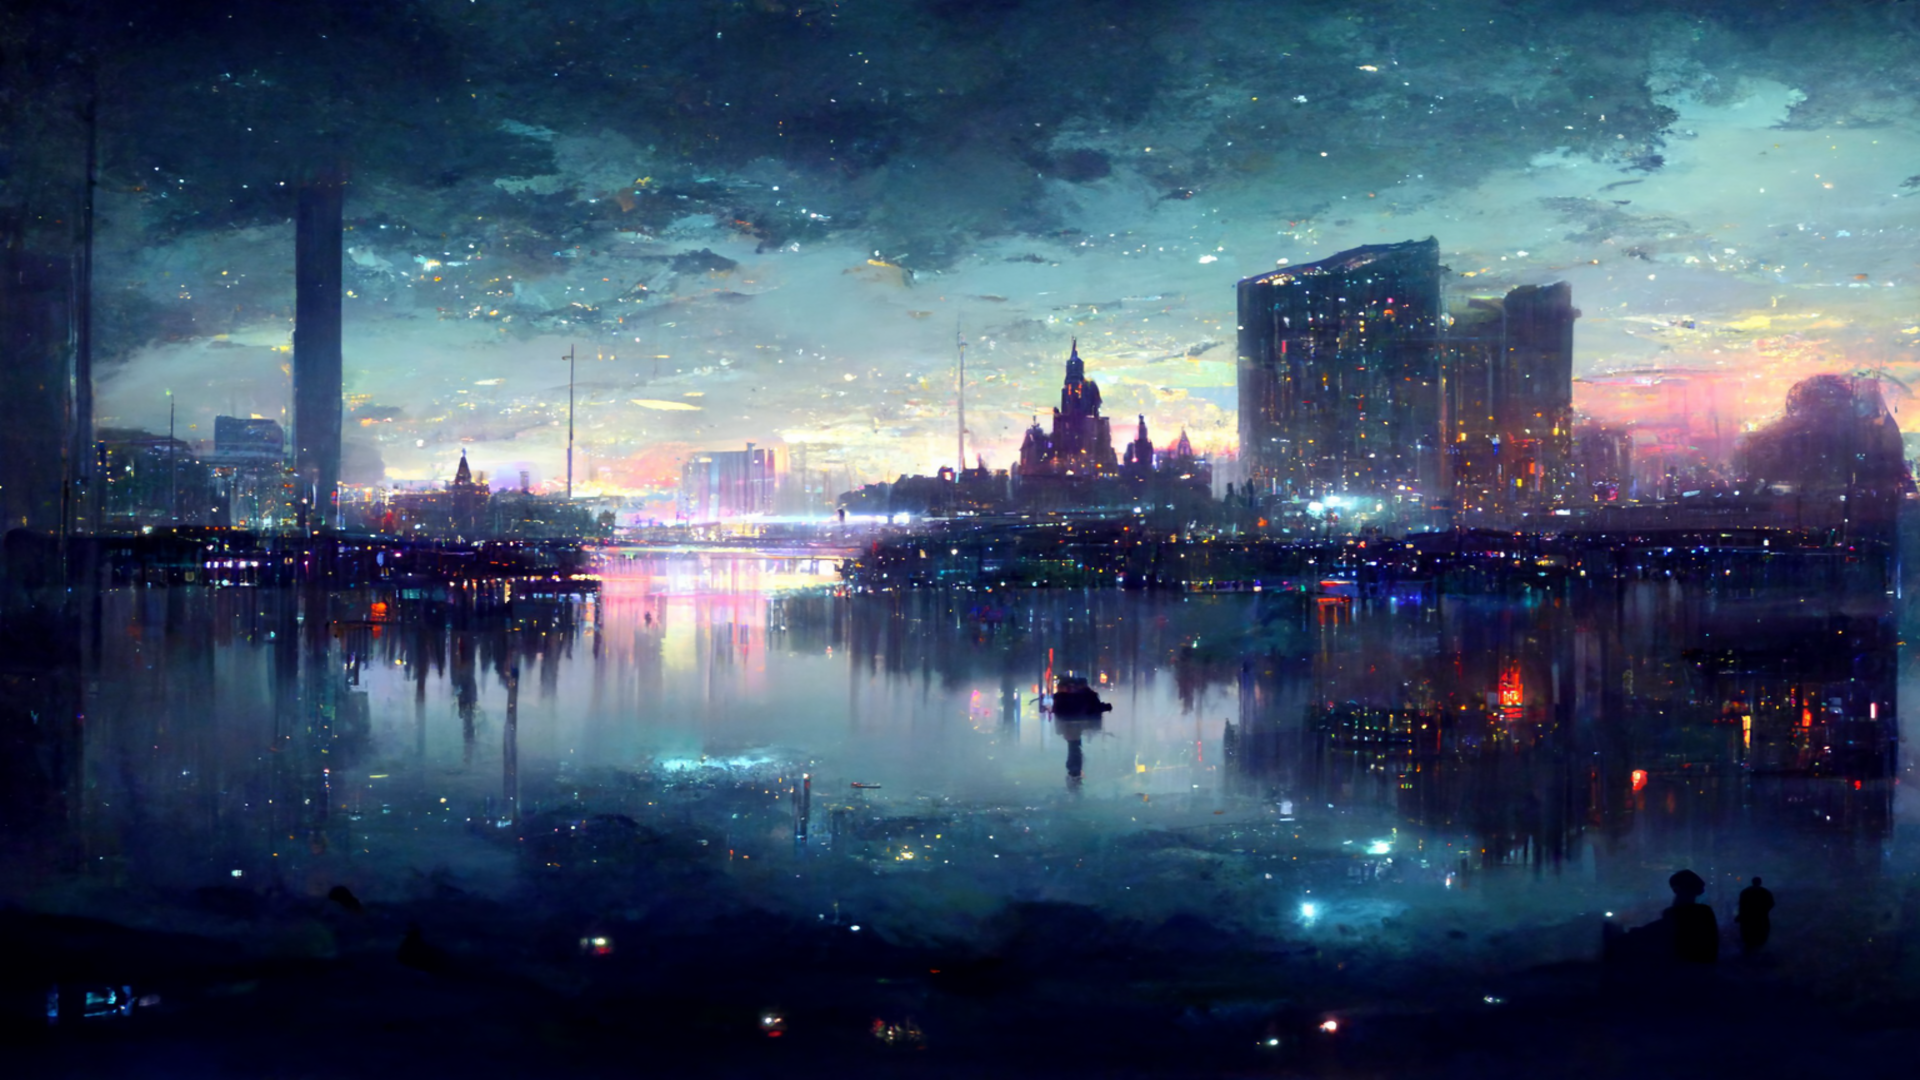
\includegraphics[width=1\textwidth]{images/background/Pixiv-101752160_p1.png}
    \end{subfigure}
    \caption{Background images\cite{101510980}\cite{100810147}\cite{101735564}\cite{101752160}}
\end{figure}
% ================================================================================================= 
        \subsection{Evolving Hyperparameter}
        Hyperparameter is the type of parameter whose values govern the entire deep learning model's learning process. 
        Furthermore, it determines the values of model parameters that a learning algorithm ends up learning, despite not being a part of the deep learning model.

        Hyperparameter evolution is a method of hyperparameter optimization that employs a Genetic Algorithm (GA) for optimization.
        In machine learning, hyperparameters control numerous elements of training, and finding optimal values for them may be complex. 
        Traditional approaches, such as grid searches, can soon become intractable owing to the large dimensionality of the search space, unknown relationships across dimensions, and the costly aspect of evaluating fitness at each point, making GA a viable choice for hyperparameter searches\cite{EvolvingHyperparameter}.
% ================================================================================================= 
        \subsection{Traning and Inference}
            Through training, data is fed into the model to produce a better-trained model. The new weight is then used to infer unlabeled images. That made the labeling procedure faster and less tedious.
%           ================================================================================================= 
        \subsection{Manually Check Label}
            After all of the images have been processed, the 
            identity of each face within each image will be manually checked and adjusted using \textbf{labelImg}\cite{labelimg} to set a better standard for the 
            face detection model. These images along with the bounding box and identity 
            data will then be used for our face identification model. The restrictions for the bounding box span from the top of the head to the chin and ear-to-ear; if they have certain unique accessories, those are also included.
% ================================================================================================= 
        \subsection{Label Format}
            YOLOv5 Pytorch has a highly unique label format. (\autoref{fig:yolov5format}). 
            Therefore, this format must be converted to another standard format, like Pattern Analysis Statistical Modeling and Computational Learning Visual Object Classes (Pascal VOC)\cite{pascalvoc} or Common Objects in Context (COCO)\cite{coco} (\autoref{fig:otherformats}), when interacting with other processes, like rotation in augmentation.
            For this reason, a different sub-program called \textbf{Bounding Box Converter}\cite{boundingboxconverter} was developed using the formulas shown in \autoref{fig:conversionformula}. Here is the snippet of how it was implemented: \autoref{fig:thefillerarc}.
        \label{Chapter Experiment} 
\section{Experiment}
    \subsection{Final Dataset}
        In the final cycle, 10938 images were used for training and 2683 images for validating (\autoref{table:DatasetInformation}). 2464 images (with 80\% for training, 20\% for validating, and 0\% for testing) from all the sources listed above were used to generate 9856 augmented images. The original dataset has inconsistent number of labels for each class (\autoref{chart:Originaldatasetlabeldistribution}) but the splitting algorithm has done a great job to balance out the number labels per class for training set (\autoref{chart:Trainingsetlabeldistribution}) and validating set (\autoref{chart:Validatingsetlabeldistribution}). Additionally, there are 1301 background images (equivalent to 10\% of the dataset) chosen for each sub-set.

        For the number of instances of each class, there were 41 for training and around 9 for validating from the original dataset (\autoref{table:LabelDistribution} and \autoref{table:LabelDistribution1}). 
        After that, all of that expanded into 164 more labels per class for training and 36 for validating.
    \subsection{Final Hyperparameter Evolving}
        The configuration described in \autoref{table:Configuration} was used for the final evolution.
        The program took 10 days to finish running and return the results in \autoref{table:Hyperparameters}.
    \subsection{Final Training}
        For the last training session, the configuration listed in \autoref{table:Configuration} was employed. The YOLOv5x6 architecture and the customized version of hyperparameter are chosen with a preference for high accuracy.The results are shown in \autoref{fig:result1}, \autoref{fig:result2}, and \autoref{fig:result3}.
    \subsection{Deploy}
        For the sake of demonstration, \textbf{YOLOv5 Hololive Waifu Detection}\cite{Application} application was made. \textbf{Streamlit} is used for a basic GUI, and the application is hosted on the \textbf{Hugging Face Spaces} (\autoref{fig:WebApp}).
        Hugging Face Spaces offer a straightforward website to host machine learning demonstration applications directly. 
        Streamlit and Gradio are two fantastic Python SDKs that are supported by the platform. 
        Users may also construct static Spaces with JavaScript and HTML for more personalized demonstrations\cite{huggingfacespaces}.
    \end{multicols}
    \clearpage   
        \label{Chapter Conclusion And Future Works}
    \begin{multicols}{2}
        \section{Conclusion And Future Works}
            Future work will be further improved upon by scraping and feeding data from each talent's alternative outfits to our model since each talent has various kinds of outfits and decorations. 
            \autoref{fig:modelvariation} is an example of completely different official outfits for Uruha Rushia.
            \label{Figure Model Variation}
\begin{figure}[H]
    \centering
    \begin{subfigure}{0.17\textwidth}
        \centering
        
\includegraphics[width=\textwidth]{images/variation/ru1.jpg}
        \caption{Original\cite{rushiaoriginal}}
        \label{fig:ru1}
    \end{subfigure}
    \hfill
    \begin{subfigure}{0.17\textwidth}
        \centering
        
\includegraphics[width=\textwidth]{images/variation/ru2.jpg}
        \caption{Alternative\cite{rushiaalternative}}
        \label{fig:ru2}
    \end{subfigure}
    % \begin{flushleft}
    %     (a) Original outfit\\
    %     (b) Alternative outfit
    % \end{flushleft}
    \caption{Model variation}
    \label{fig:modelvariation}
\end{figure}
            Also, there are many niche cases, such as different angles, real cosplay, characters' outfits swapping, or numerous art styles (\autoref{fig:niche}), that are not in our dataset at the moment.
            
            Furthermore, we hope to develop a tool that will be capable of classifying all virtual YouTubers. Aside from Hololive, there are numerous other agencies (Nijisanji, VShojo, VirtuaReal, etc.) as well as independent VTubers.
        
            Under-sampling is the data splitting method used. However, this approach will not utilize all the available images in the collected dataset. 
            A customized over-sampling algorithm will therefore be included in the upcoming version to resolve this concern. 
            The brief idea is to generate more images using various augmentation techniques to balance the number of labels in each class.

            Last but not least, other helpful augmentation methods (such blur, color channels witching, and etc) will be introduced in the future for further generalization of dataset.
            \begin{figure}[H]
    \centering
    \begin{subfigure}{0.2\textwidth}
        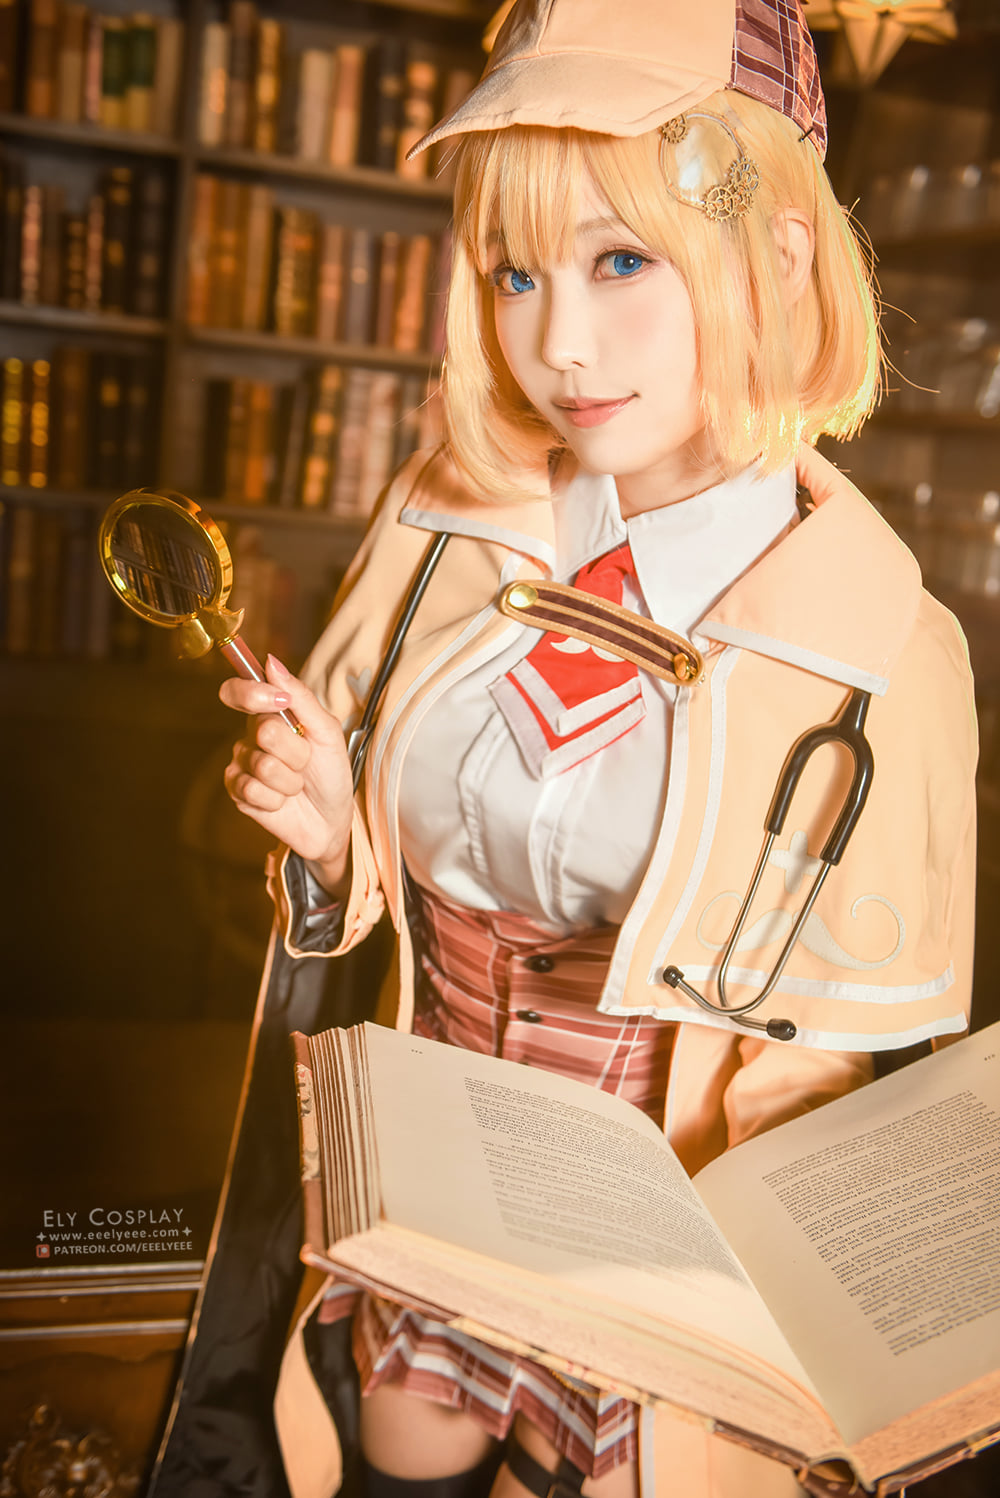
\includegraphics[width=\textwidth]{images/niche/243977316_423878135766209_1700862170532318412_n.jpg}
        \caption{Cosplay\cite{watsoncosply}}
    \end{subfigure}
    \hfill
    \begin{subfigure}{0.2\textwidth}
        
\includegraphics[width=1.3\textwidth]{images/niche/a7u9n4nsnwv51.jpg}
        \caption{Outfit swapping\cite{outfitswapping}}
    \end{subfigure}
    \hfill
    \begin{subfigure}{0.2\textwidth}
        
\includegraphics[width=\textwidth]{images/niche/Pixiv-82353068_p5.png}
        \caption{Unusual angle\cite{unusualangle}}
    \end{subfigure}
    \hfill
    \begin{subfigure}{0.2\textwidth}
        
\includegraphics[width=1.5\textwidth]{images/niche/Pixiv-92177593_p0.png}
        \caption{Different artstyle\cite{chibi}}
    \end{subfigure}
    \hfill
    \caption{Uncovered situations}
    \label{fig:niche}
\end{figure}

    \end{multicols}
% \clearpage
        \label{Chapter Contribution}
\section{Contribution}
% \newpage
\begin{table}[H]
\label{Table Contribution}
\caption{\label{Contribution}Contribution distribution.}
    \begin{center}
        \begin{tabular}{ | m{15em} | m{4em}| m{4em} | m{4em} | } 
            \hline
                \centering\textbf{Task} & 
                \centering\textbf{Khoa} & 
                \centering\textbf{Hung} & 
                \centering\textbf{Khoi} 
                \tabularnewline
            \hline
                \texttt{Data Gathering} &
                \centering\textbf{x} &
                \centering\textbf{x} &
                \centering\textbf{x}
                \tabularnewline
            \hline
                \texttt{Label Images} &
                \centering\textbf{x} &
                \centering\textbf{x} &
                \centering\textbf{x}
                \tabularnewline
            \hline
                \texttt{Label Checking} &
                \centering\textbf{x} &
                \centering\textbf{x} &
                \centering\textbf{x}
                \tabularnewline
            \hline
                \texttt{Data Preparation} &
                \centering\textbf{x} &
                \centering\textbf{} &
                \centering\textbf{}
                \tabularnewline
            \hline
                \texttt{Web Demonstration} &
                \centering\textbf{x} &
                \centering\textbf{} &
                \centering\textbf{}
                \tabularnewline
            \hline
                \texttt{Report Writing} &
                \centering\textbf{x} &
                \centering\textbf{x} &
                \centering\textbf{}
                \tabularnewline
            \hline
                \texttt{Latex Formatting} &
                \centering\textbf{x} &
                \centering\textbf{} &
                \centering\textbf{x}
                \tabularnewline
            \hline
                \texttt{Presentation Slide} &
                \centering\textbf{x} &
                \centering\textbf{x} &
                \centering\textbf{x}
                \tabularnewline
            \hline
        \end{tabular}
    \end{center}
\end{table}

\newpage
        \bibliographystyle{IEEEtran} % We choose the "plain" reference style
        \bibliography{refs} % Entries are in the refs.bib file
        \section{Appendix}
    \label{Figure BoundingBoxConversion}
\begin{figure}[H]
    \centering
    \begin{center}
        $<label>\;<xCenterScaled>\;<yCenterScaled>\;<widthScaled>\;<heightScaled>$
    \end{center}
    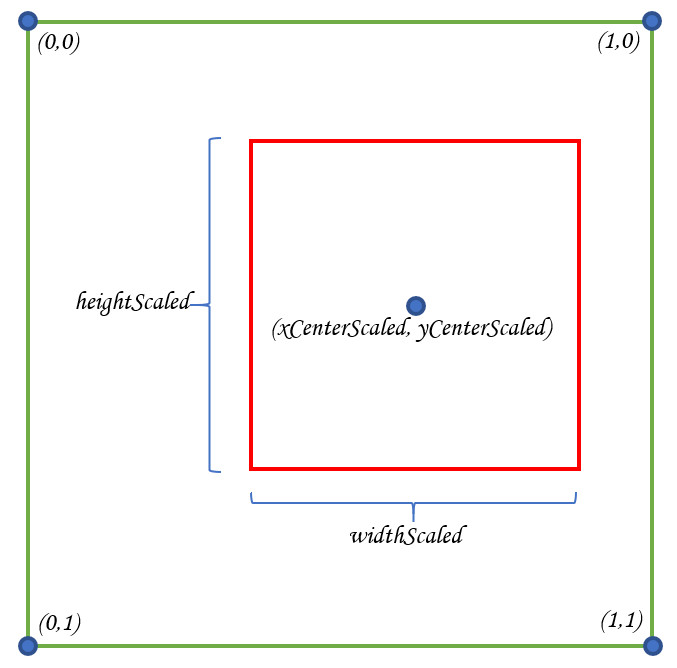
\includegraphics[width=0.5\textwidth]{images/boundingbox/BoundingBox-YOLO.jpg}
    \caption{YOLOv5 Pytorch label format}
    \label{fig:yolov5format}
\end{figure}

\begin{figure}[H]
    \centering
    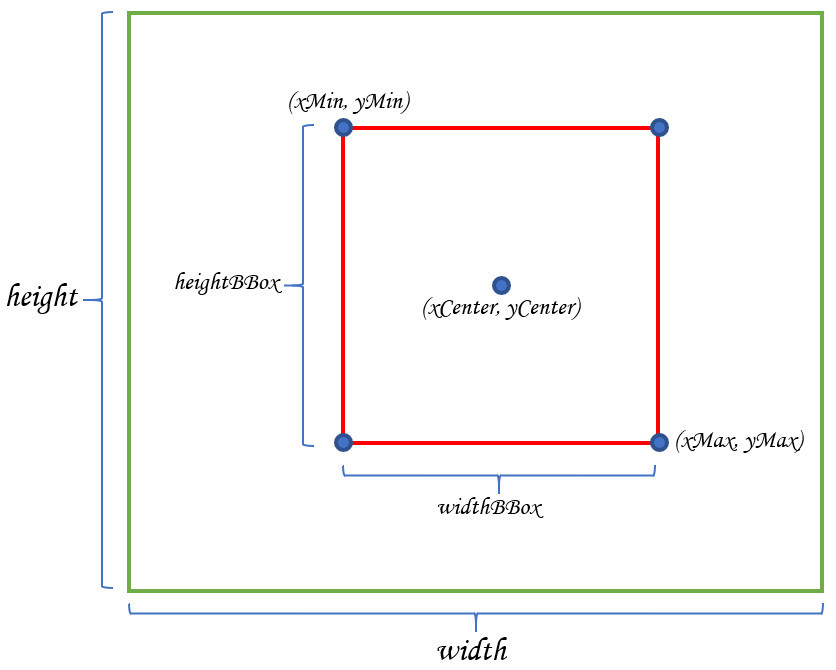
\includegraphics[width=0.7\textwidth]{images/boundingbox/BoundingBox-PascalVOC-COCO.jpg}
    \caption{Pascal VOC / COCO label format}
    \label{fig:otherformats}
\end{figure}
\clearpage

\begin{figure}[H]
    \begin{equation*}
        \begin{subfig}
            \begin{gathered}
                From\;Pascal\;VOC\;format \\
                xCenterScaled = \frac{\frac{xMin + xMax}{2} - 1}{width} \\
                yCenterScaled = \frac{\frac{yMin + yMax}{2} - 1}{height} \\
                widthScaled = \frac{xMax - xMin}{width} \\
                heightScaled = \frac{yMax - yMin}{height} \\
            \end{gathered}\hspace{6em}
        \end{subfig}
        \begin{subfig}
            \begin{gathered}
                From\;COCO\;format \\
                xCenterScaled = \frac{2 * xMin + widthBBox}{2 * width} \\
                yCenterScaled = \frac{2 * yMin + heightBBox}{2 * height} \\
                widthScaled = \frac{widthBBox}{width} \\
                heightScaled = \frac{heightBBox}{height} \\
            \end{gathered}
        \end{subfig}
    \end{equation*}
    \caption{Formulas to convert from other formats to YOLOv5 Pytorch format}
    \label{fig:conversionformula}
\end{figure}

\begin{figure}[H]
    \begin{align*}
        &xMin =\left\{\begin{matrix}
        0 \; if\; [(xCenterScaled - \frac{widthScaled}{2})*width] < 0 \\
        int([(xCenterScaled - \frac{widthScaled}{2})*width])+1 \; else,  \\
        \end{matrix}\right.\\
        &xMax =\left\{\begin{matrix}
        0 \; if\; [(xCenterScaled + \frac{widthScaled}{2})*width] > (width-1) \\
        int([(xCenterScaled + \frac{widthScaled}{2})*width])+1 \; else,  \\
        \end{matrix}\right. \\
        &yMin =\left\{\begin{matrix}
        0 \; if\; (yCenterScaled - \frac{heightScaled}{2})*height  \\
        int([(yCenterScaled - \frac{heightScaled}{2})*height])+1 \; else,  \\
        \end{matrix}\right.\\ 
        &yMax =\left\{\begin{matrix}
        height -1 \; if\; (yCenterScaled + \frac{heightScaled}{2})*height > (height-1) \\
        int([(yCenterScaled + \frac{heightScaled}{2})*height])+1 \; else,  \\
        \end{matrix}\right. 
    \end{align*}
    \caption{Formulas to convert from YOLOv5 Pytorch to Pascal VOC format}
    \label{fig:conversionformul}
\end{figure}

\begin{figure}[H]
    \centering
    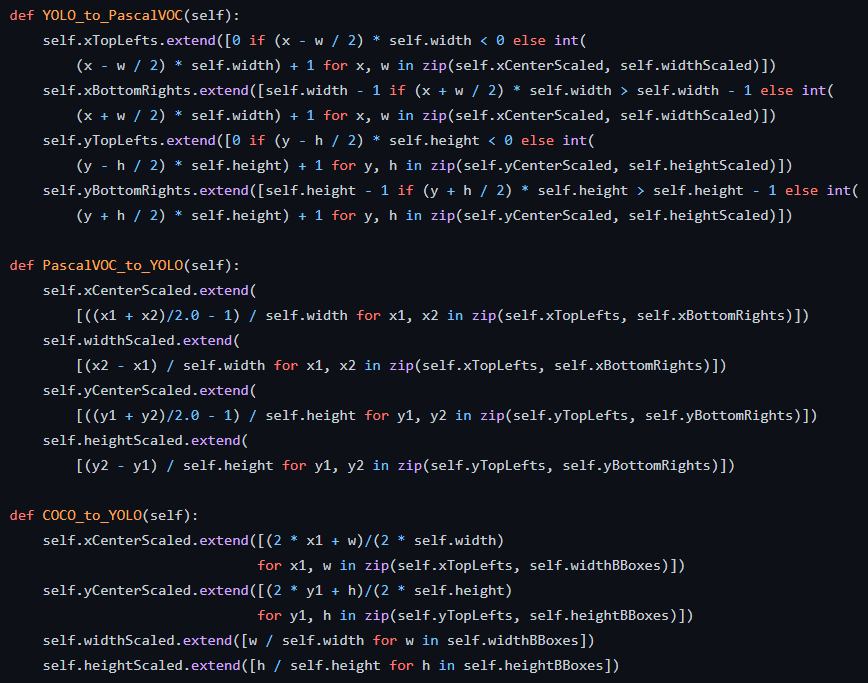
\includegraphics[width=0.75\textwidth]{images/boundingbox/CodeForBoundingBoxConversion.png}
    \caption{Code for Bounding Box Conversion}
    \label{fig:thefillerarc}
\end{figure}
    \begin{figure}
    \centering
    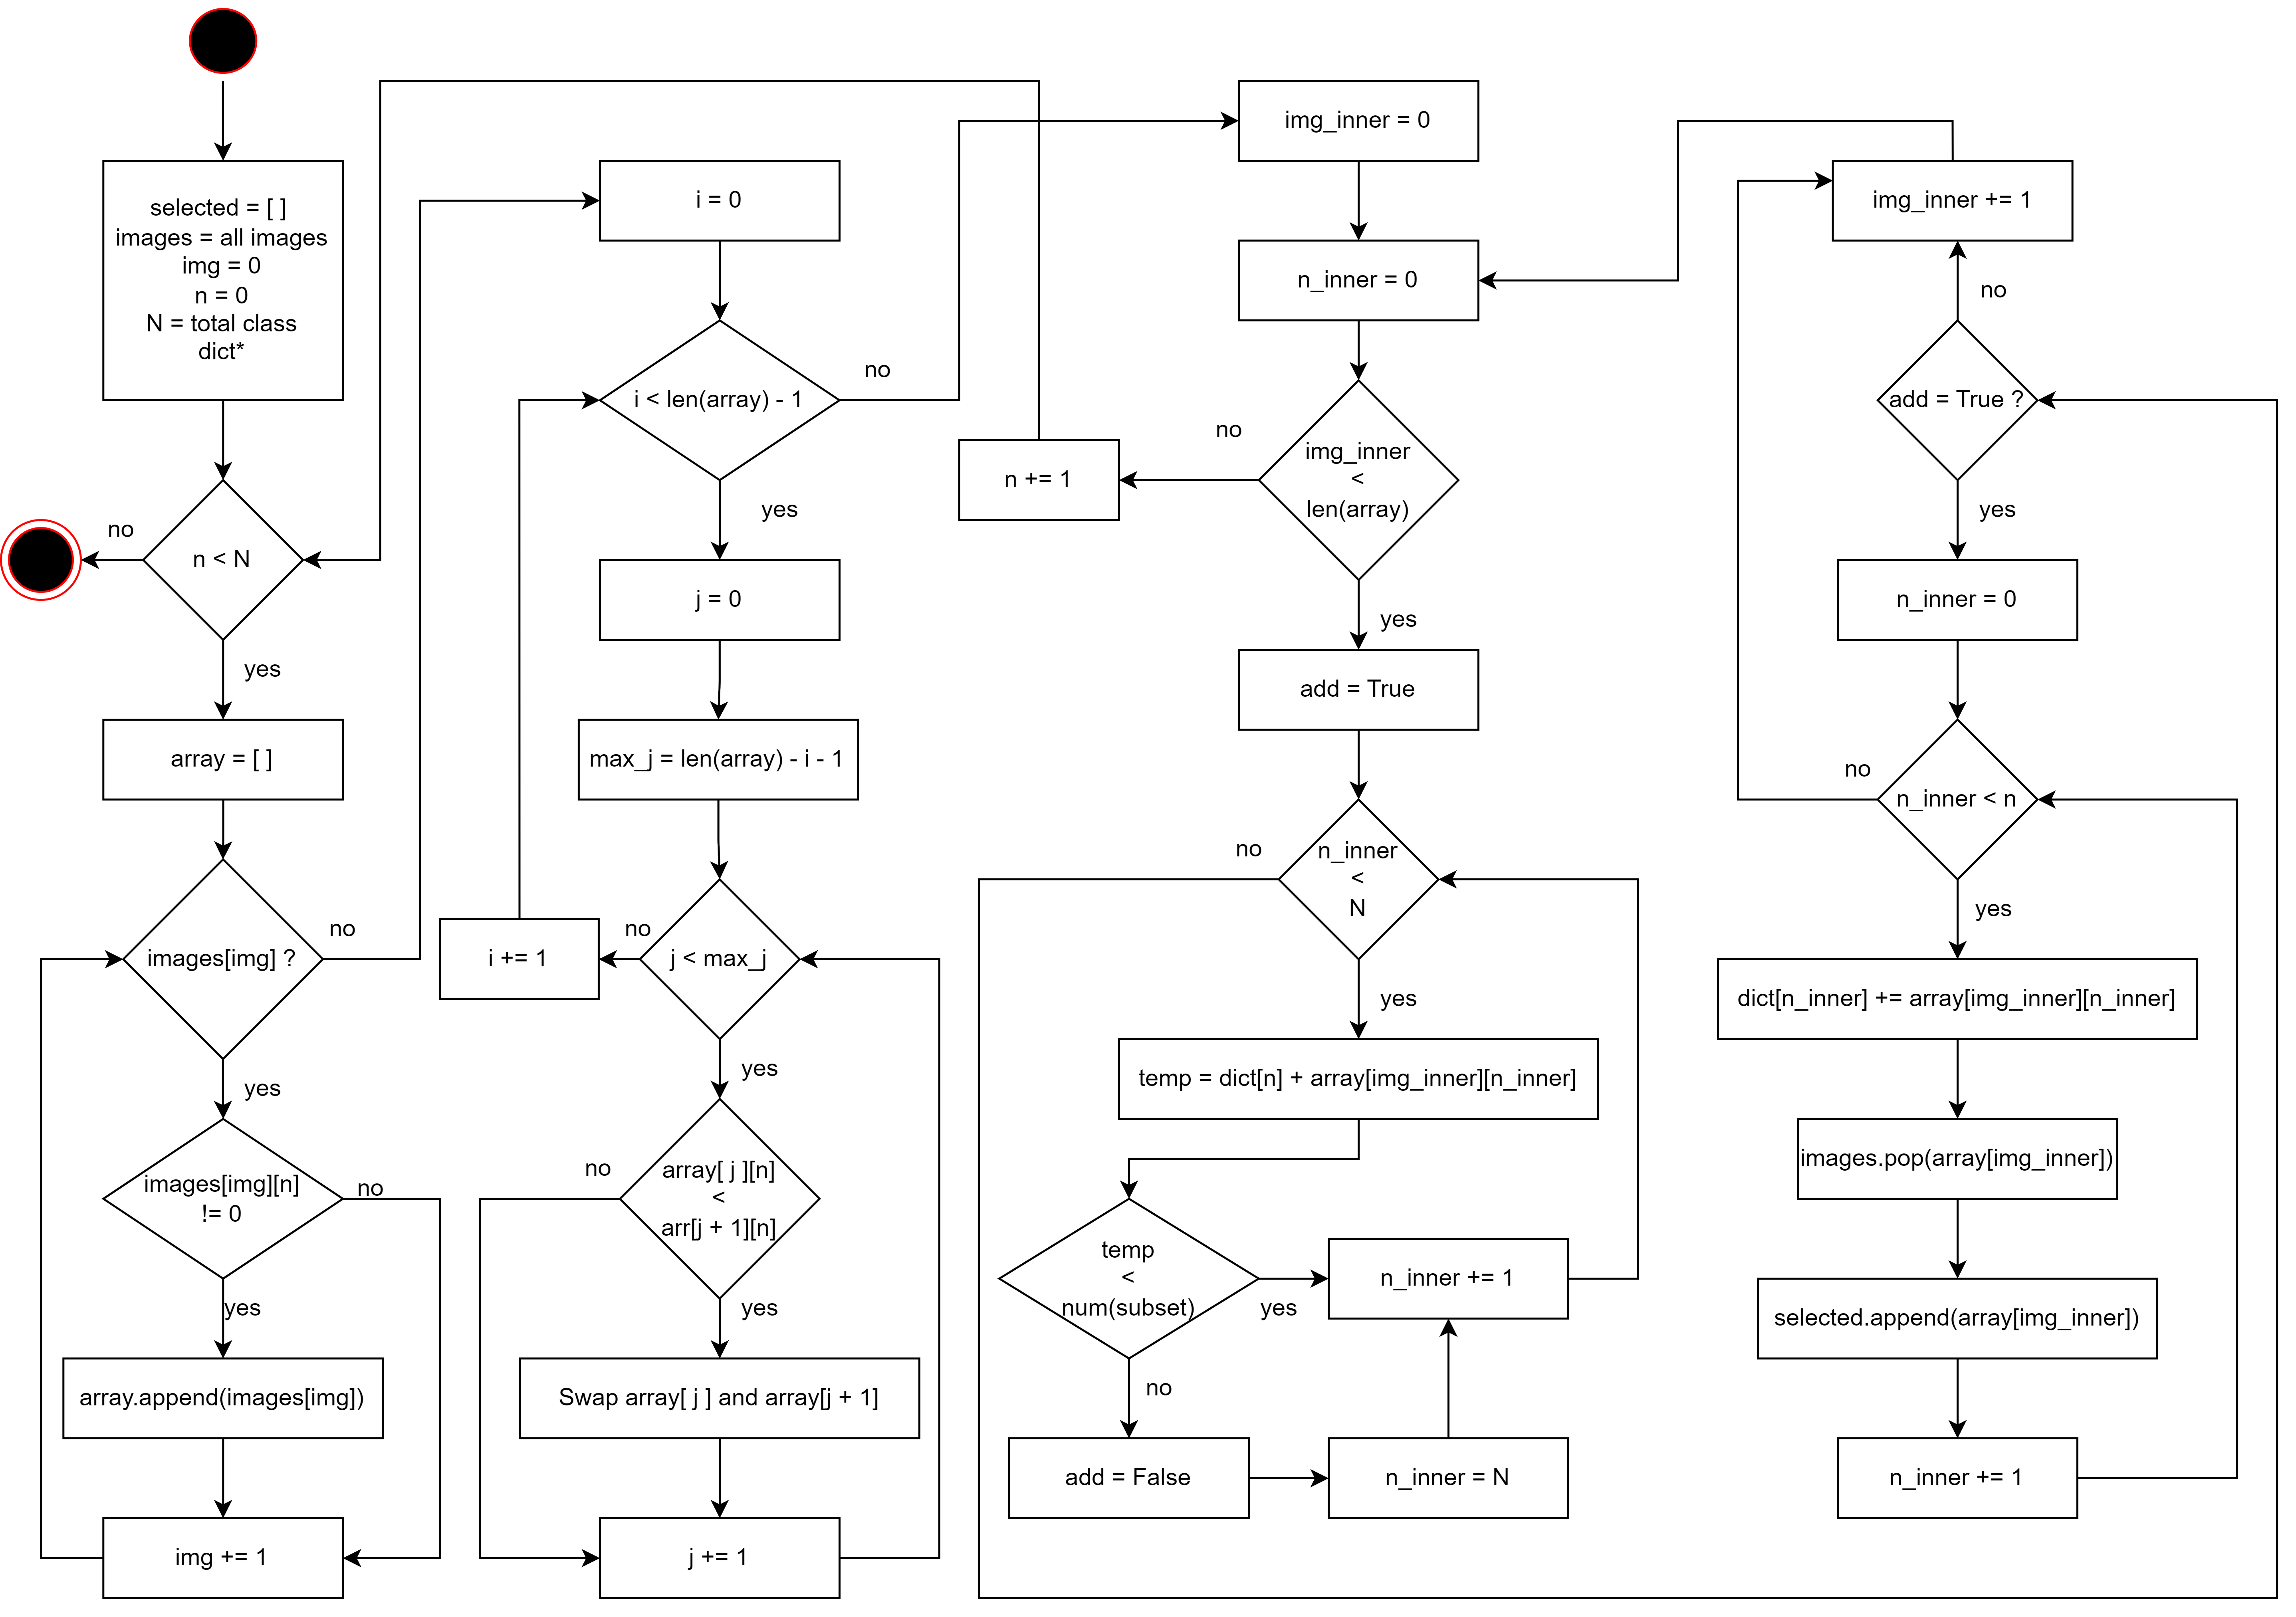
\includegraphics[width=1.3\textwidth,angle=90]{diagrams/FlowChart-Customized_UnderSampling_2.png}
    \caption{Customized UnderSampling}
    \label{fig:CustomizedUnderSampling}
\end{figure}
    \begin{figure}[H]
    \centering
    \begin{subfigure}{1\textwidth}
        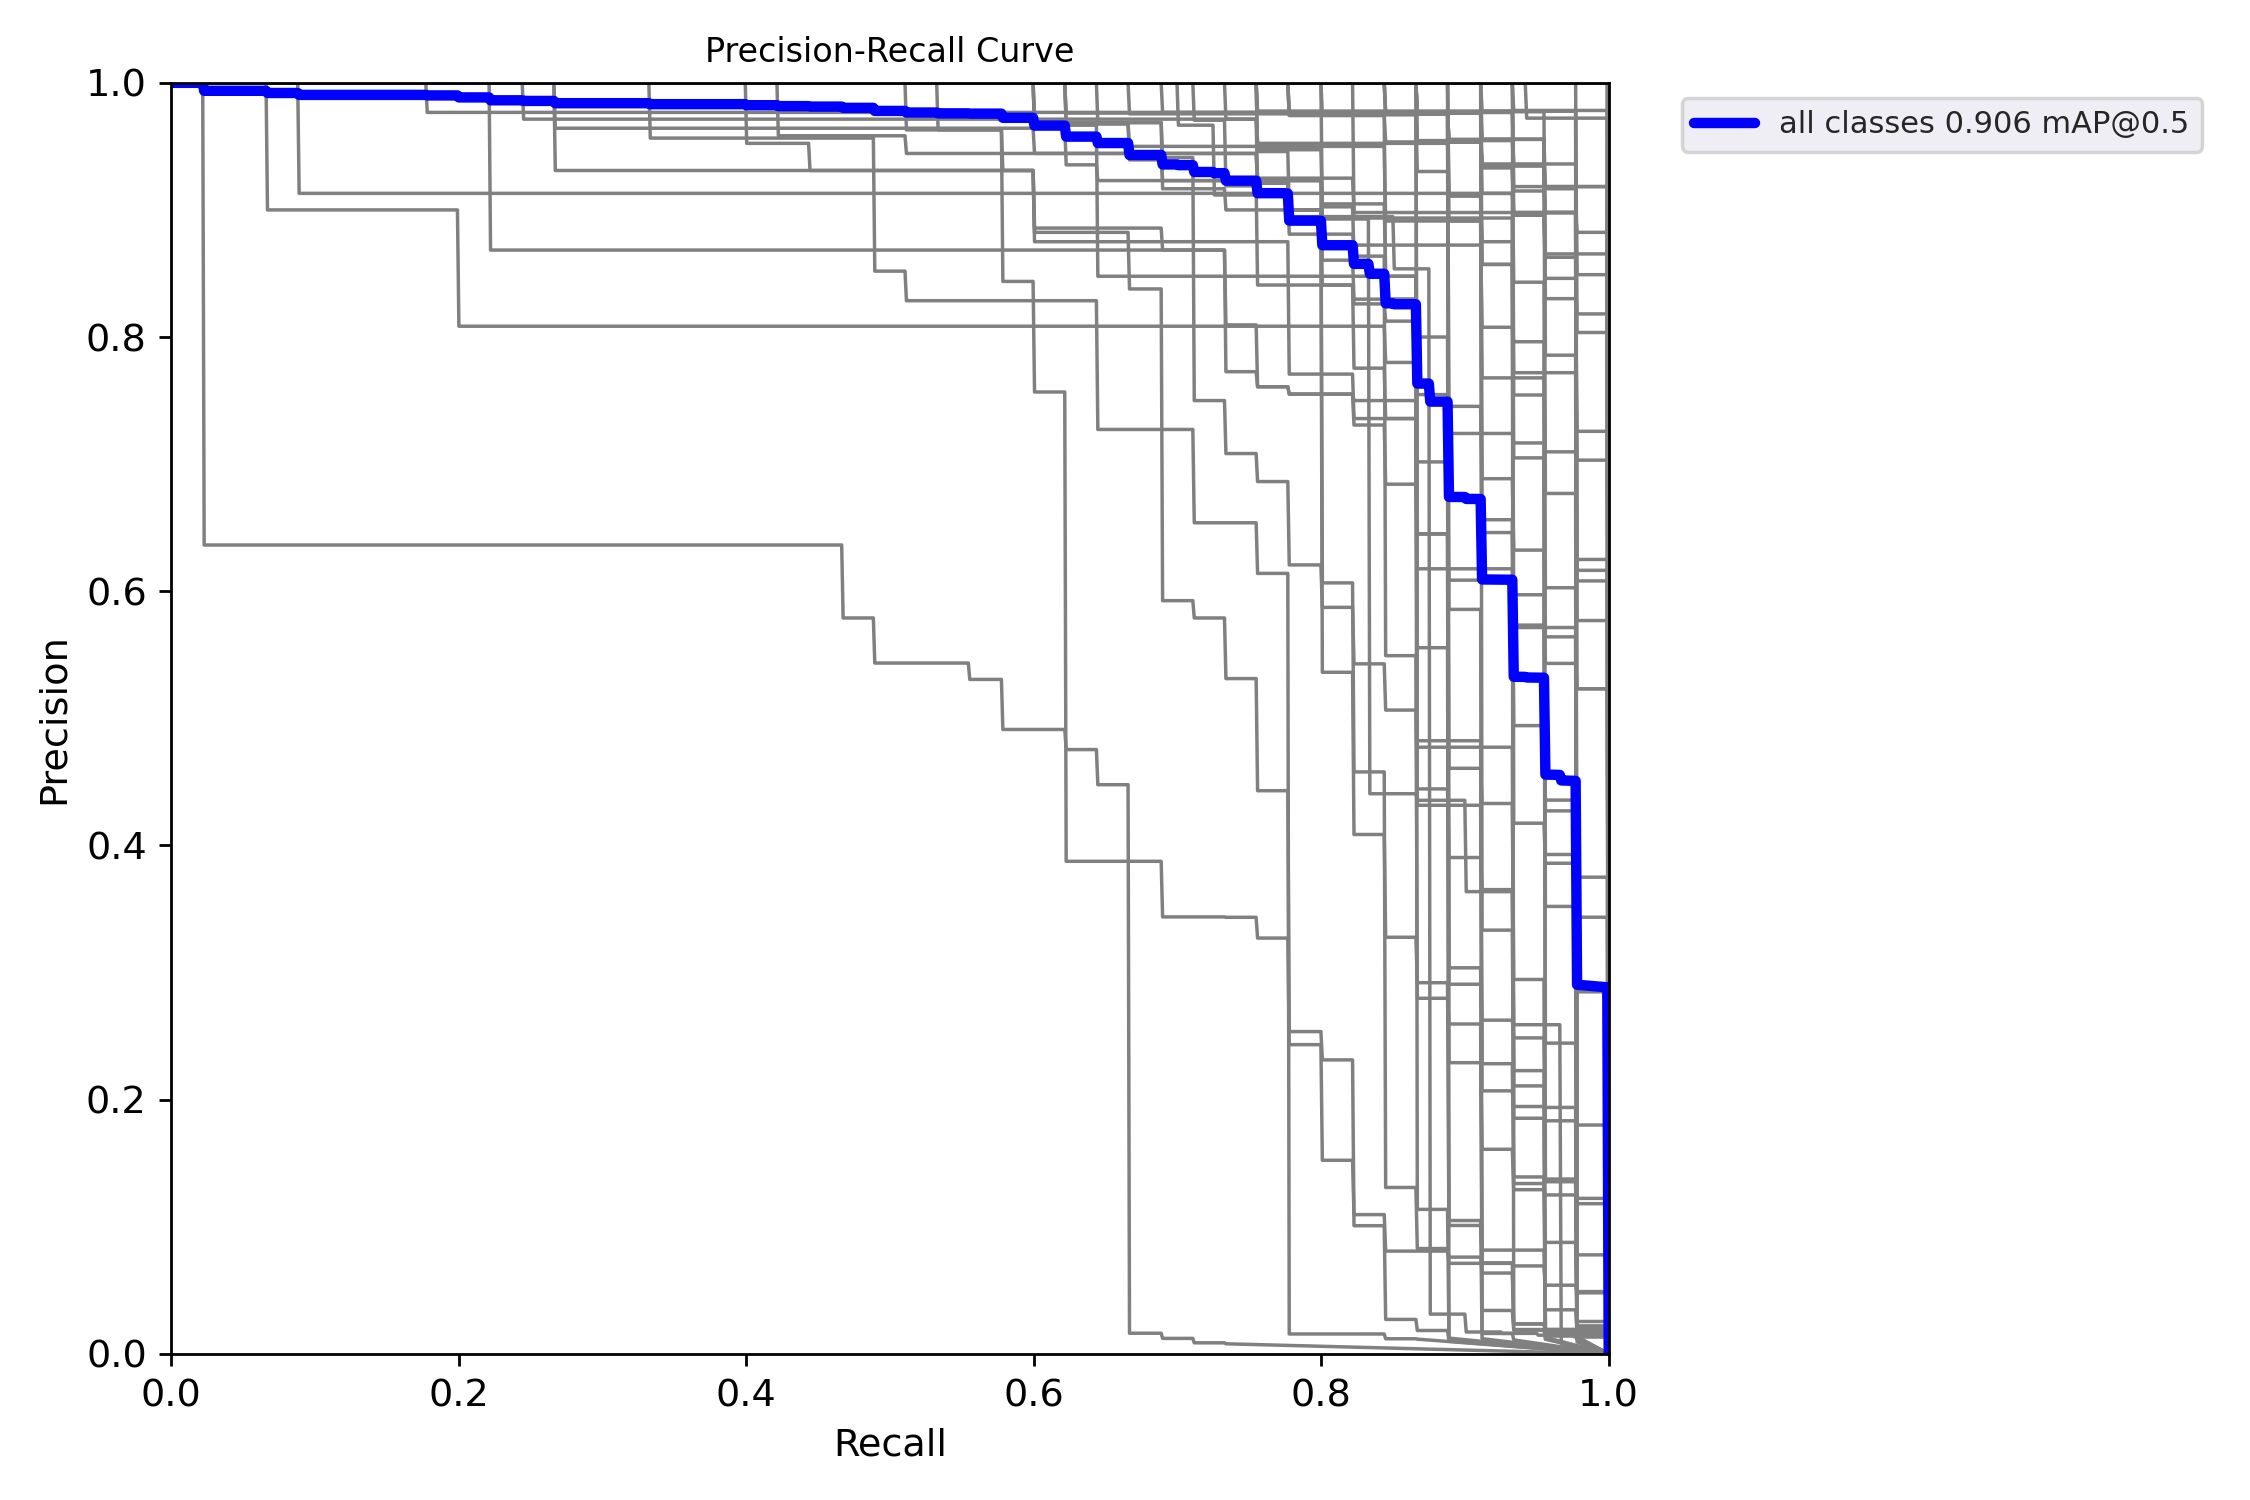
\includegraphics[width=1\textwidth]{images/results/PR_curve.png}
    \end{subfigure}
    \hfill
    \begin{subfigure}{1\textwidth}
        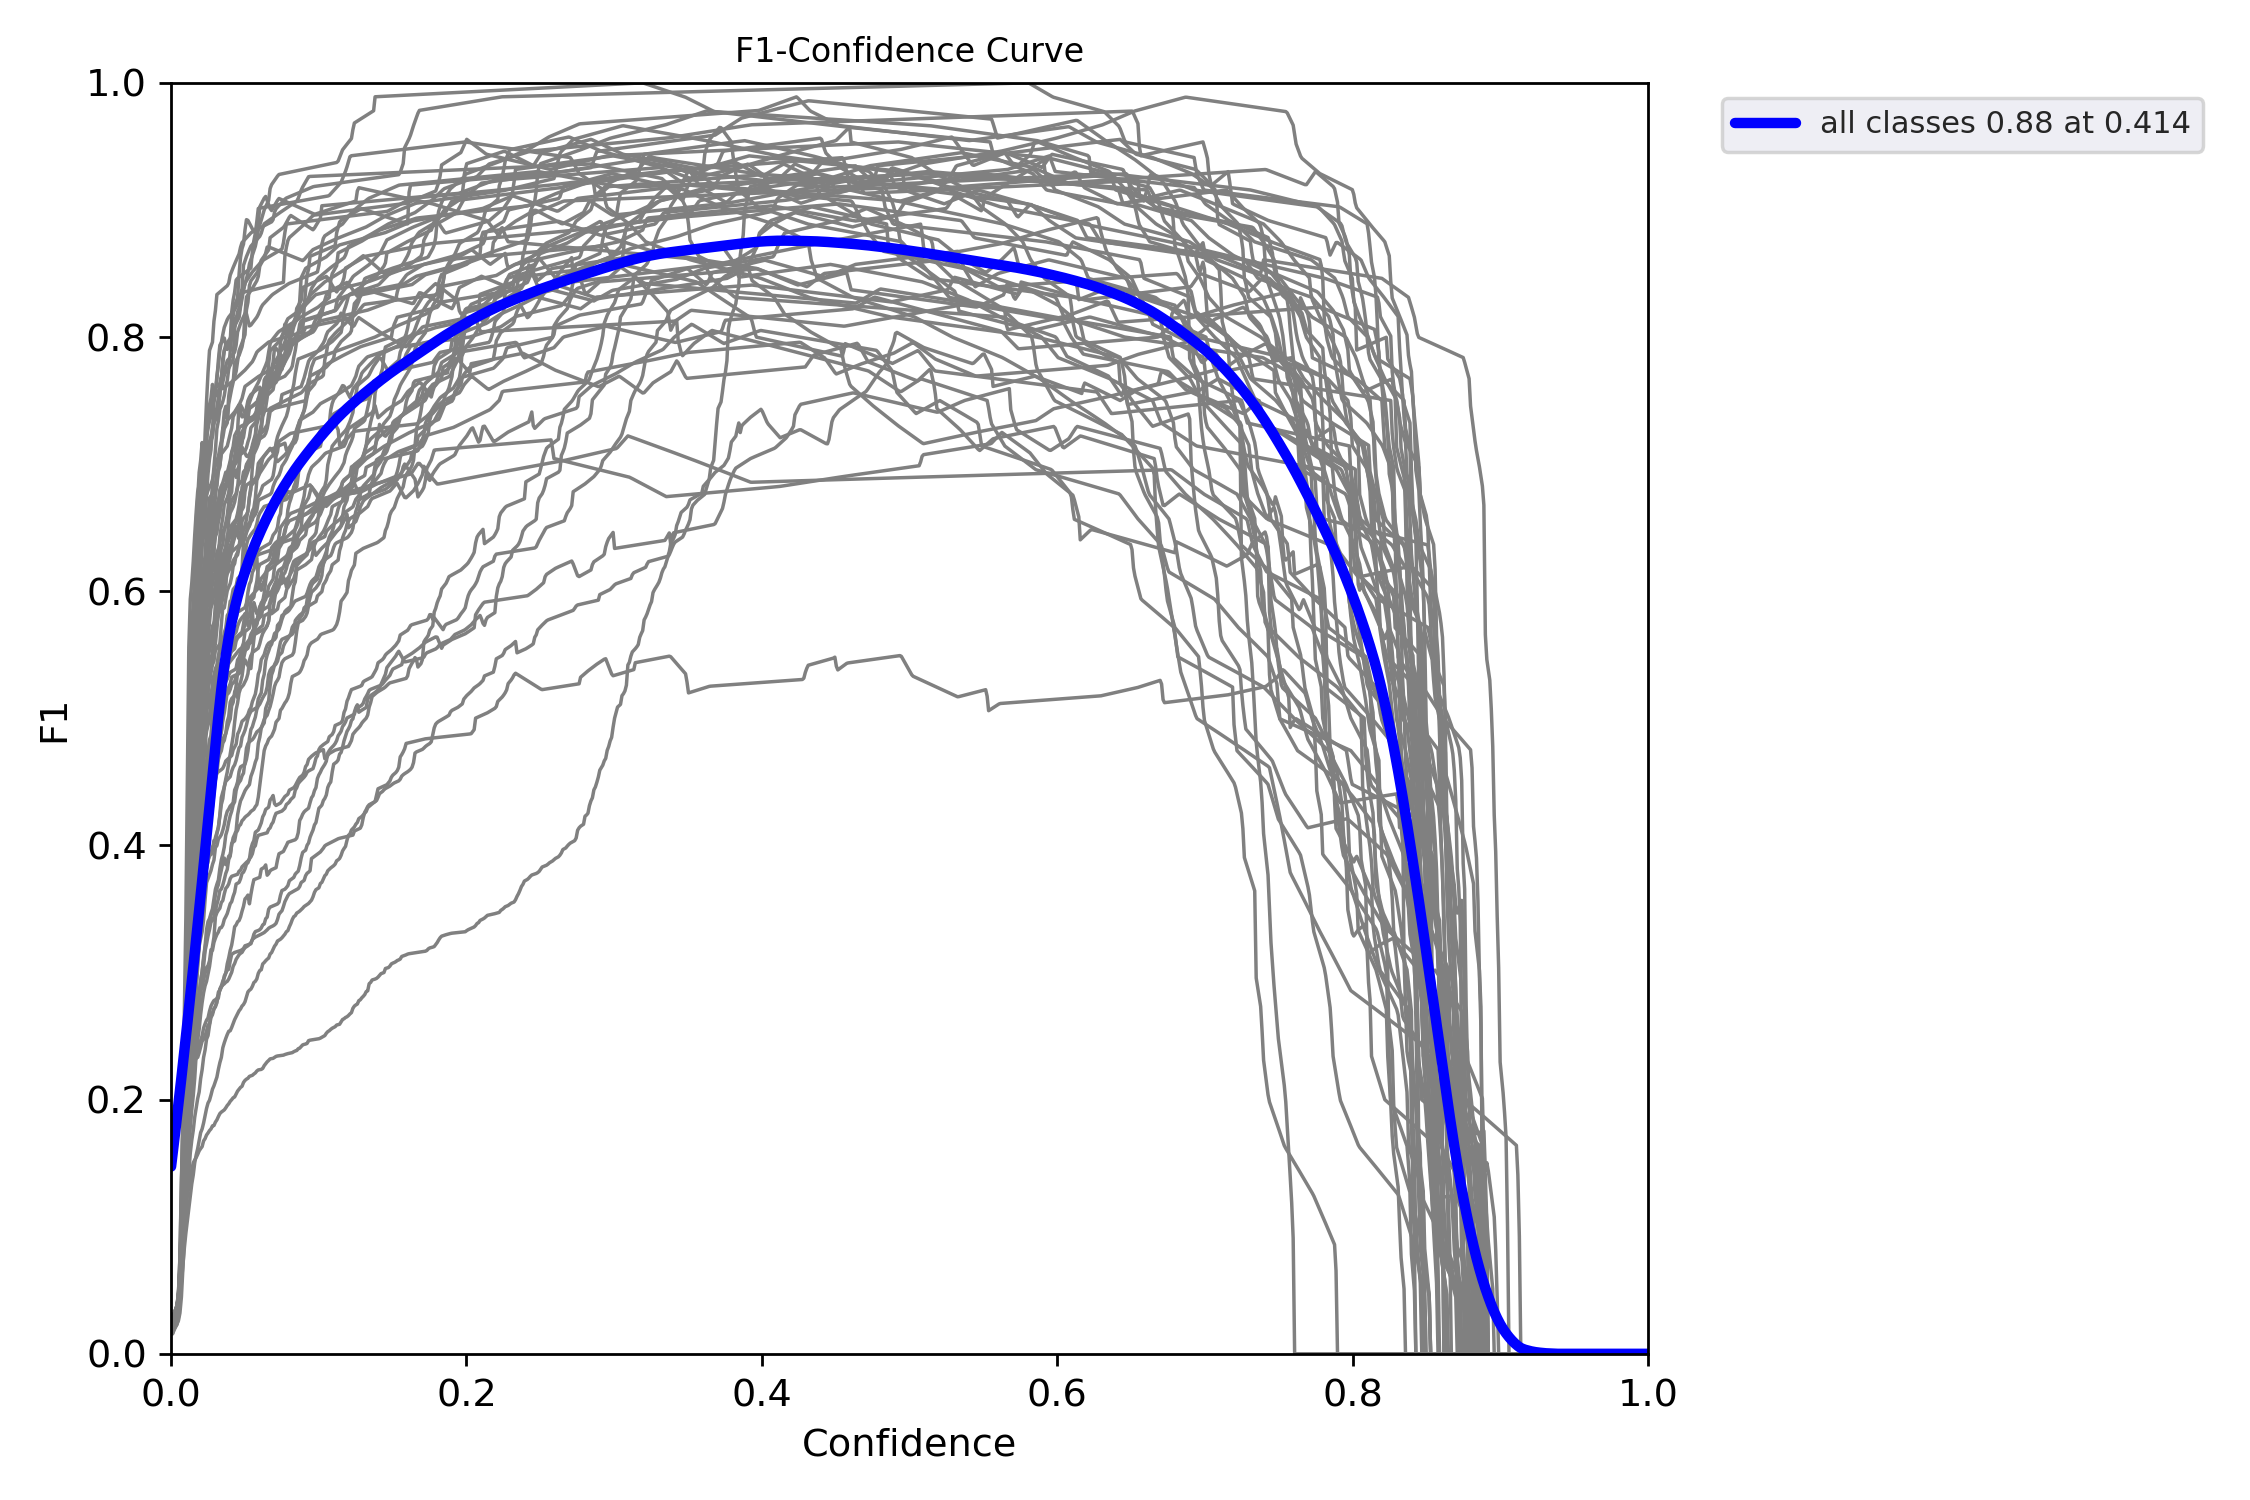
\includegraphics[width=1\textwidth]{images/results/F1_curve.png}
    \end{subfigure}
    \hfill
    \caption{Results}
    \label{fig:result1}
\end{figure}

\begin{figure}[H]
    \centering
    \begin{subfigure}{1\textwidth}
        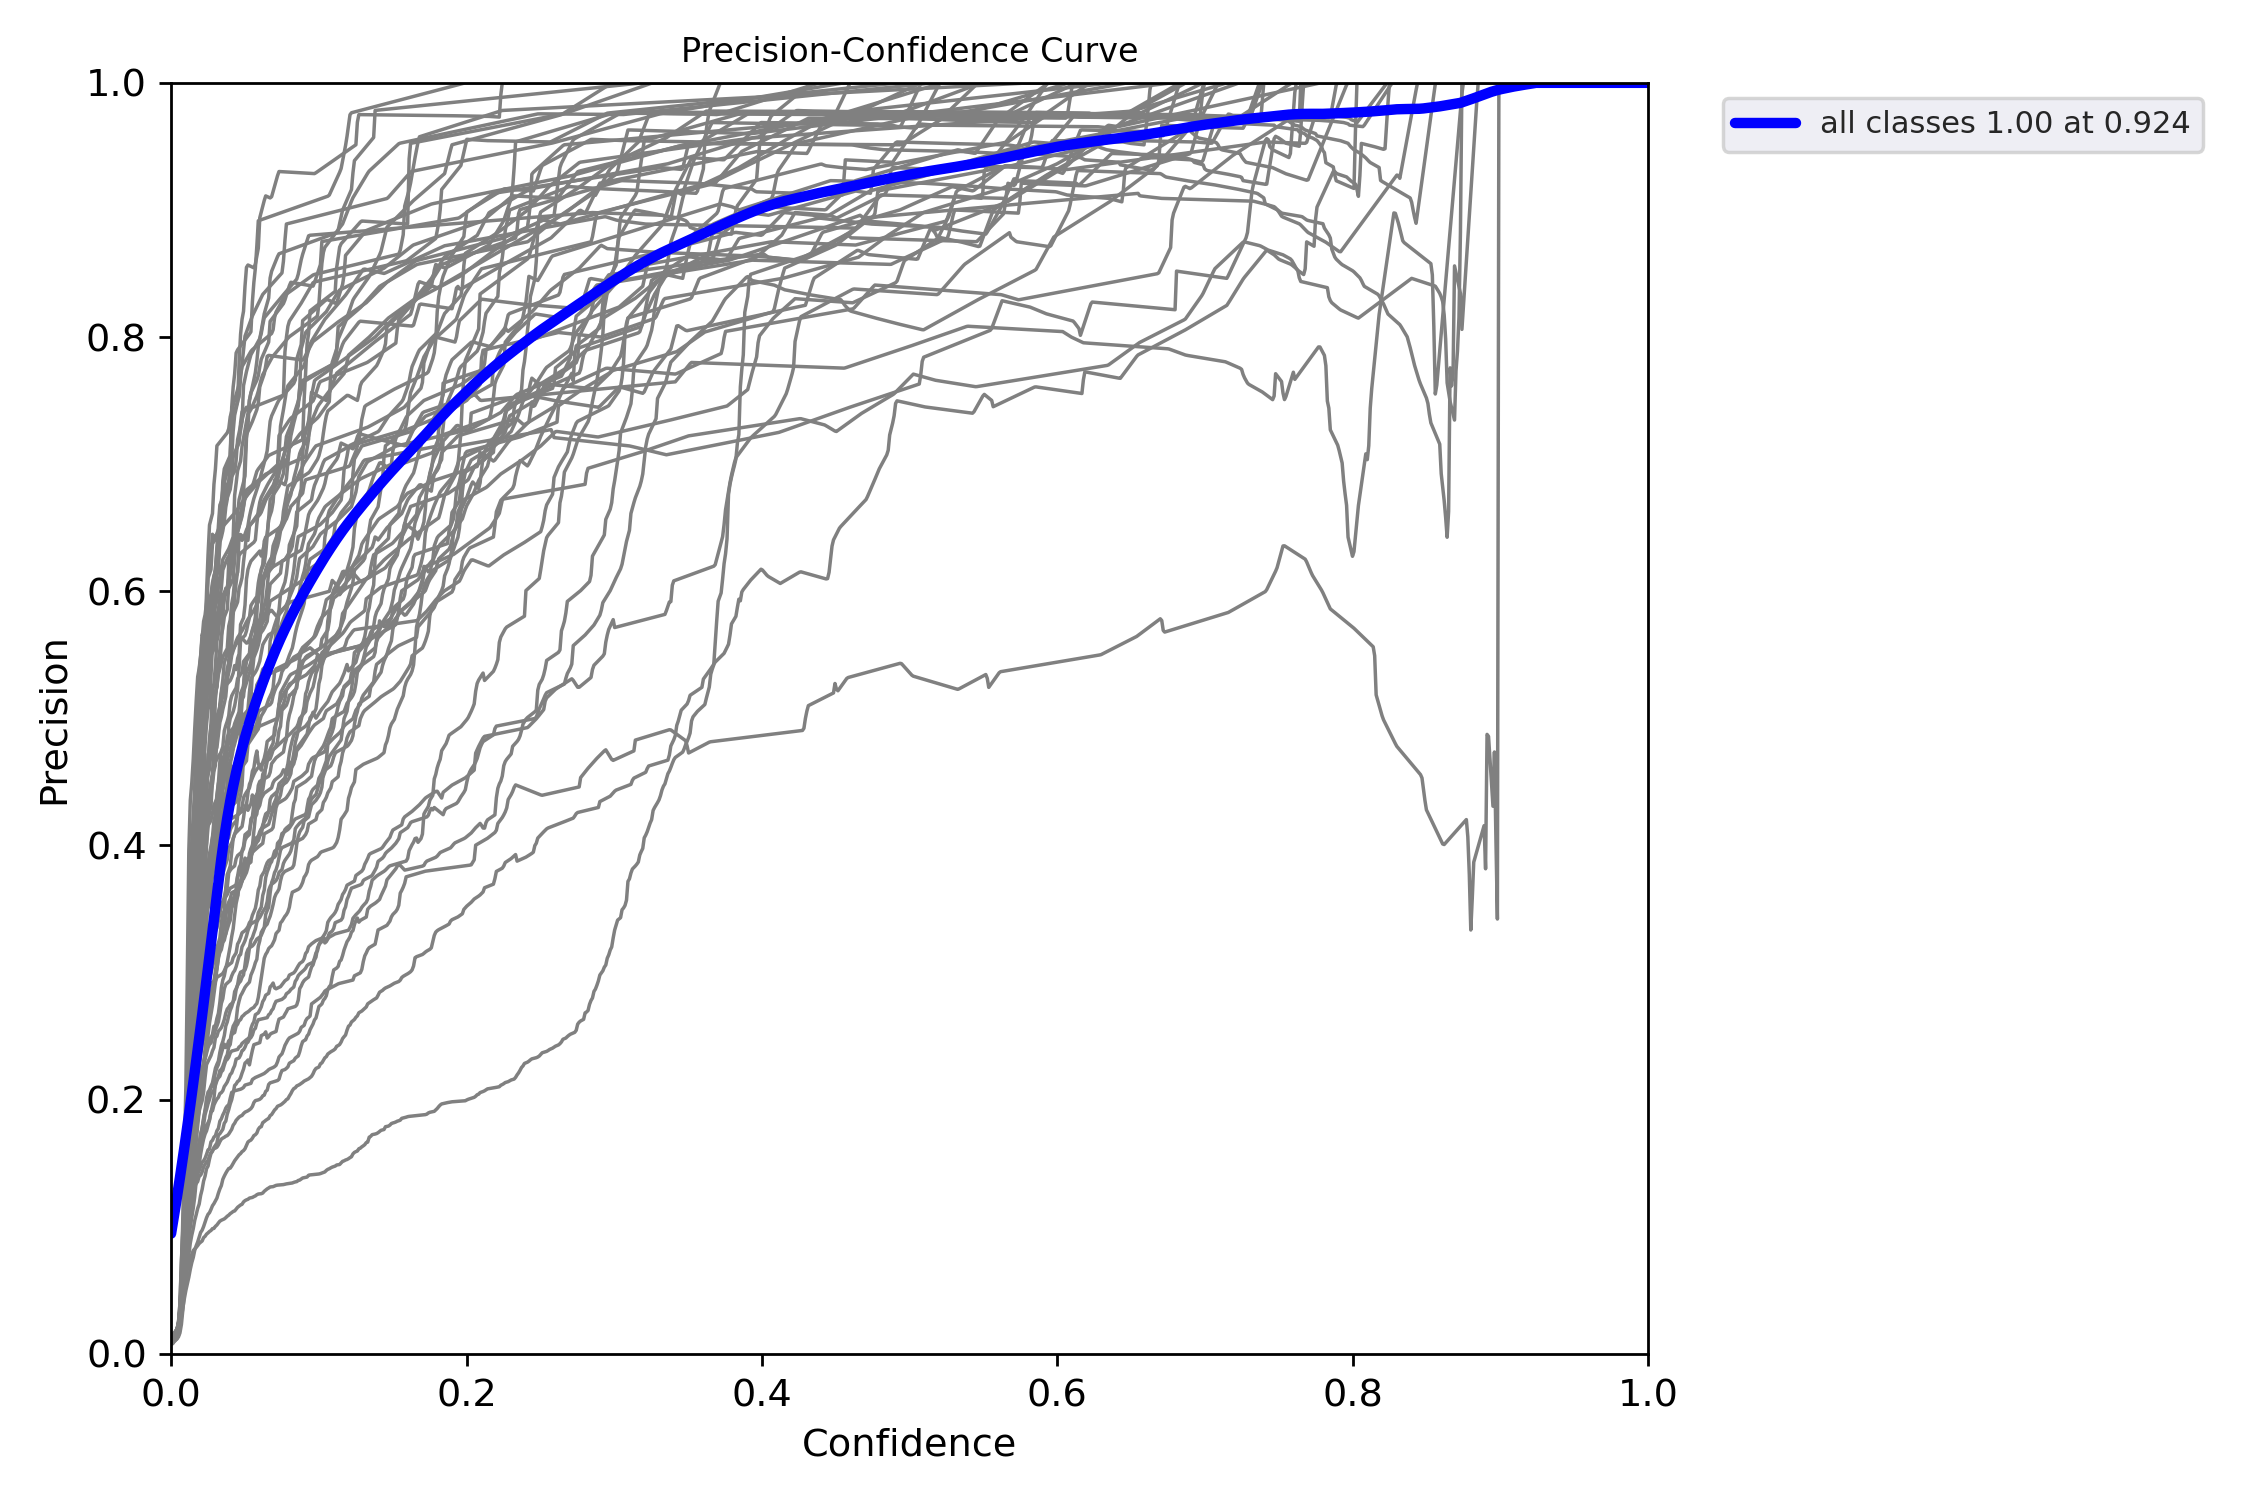
\includegraphics[width=1\textwidth]{images/results/P_curve.png}
    \end{subfigure}
    \hfill
    \begin{subfigure}{1\textwidth}
        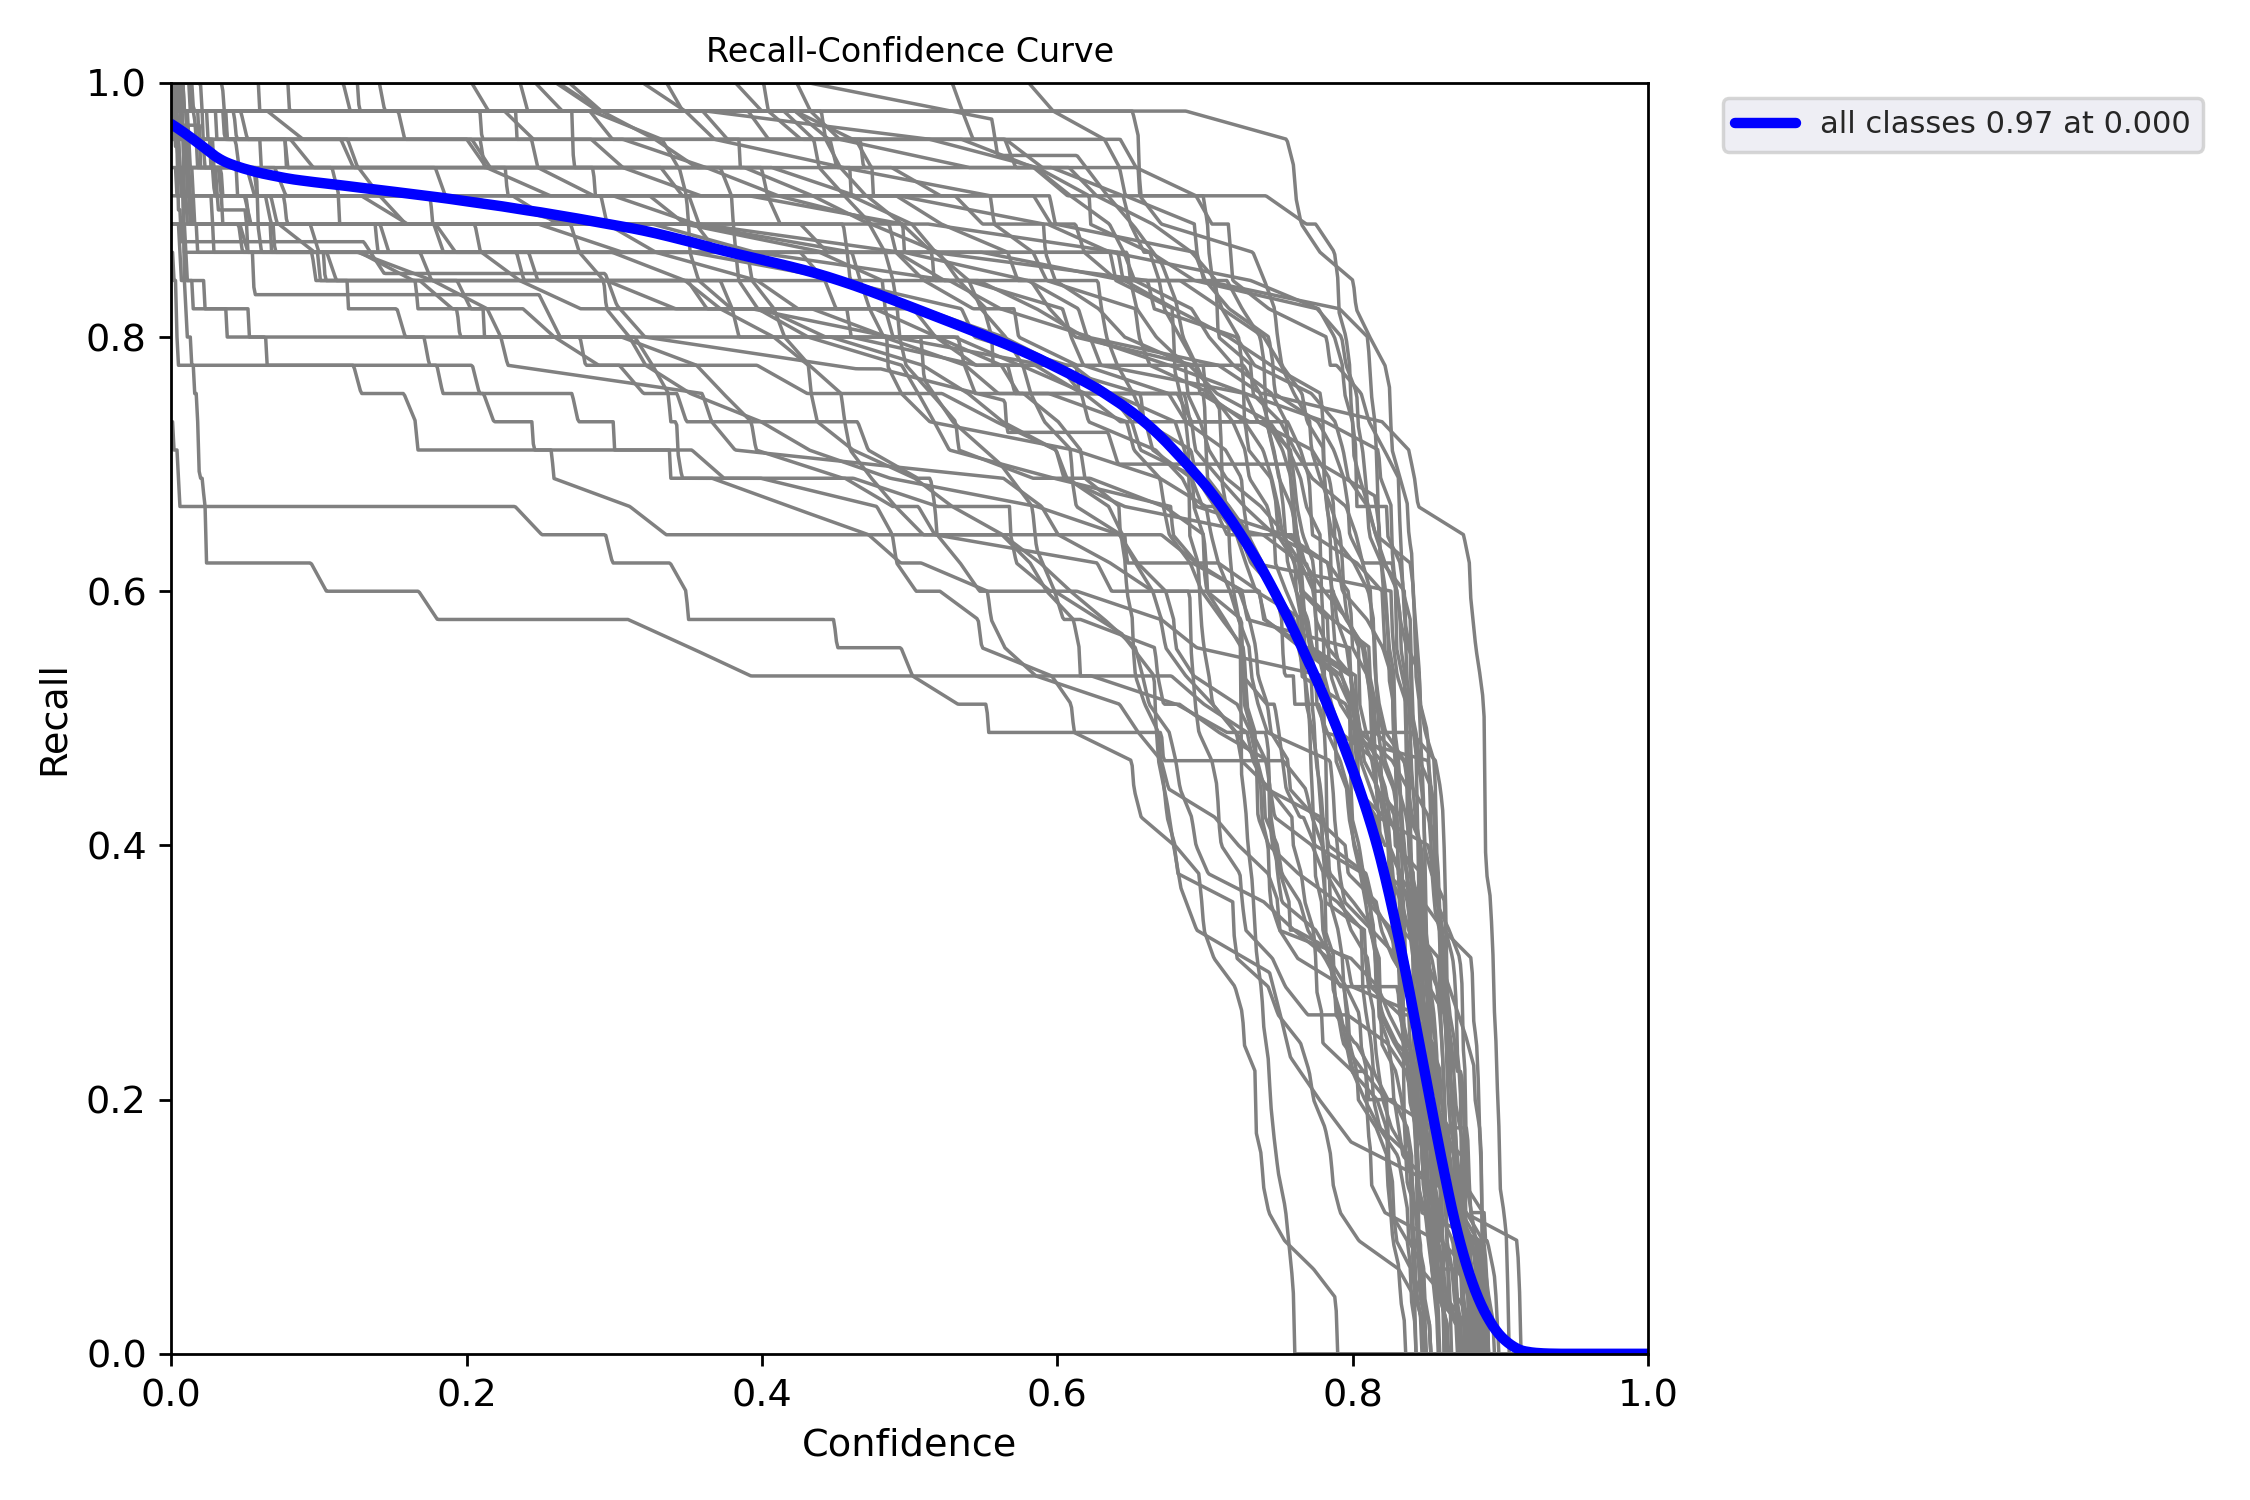
\includegraphics[width=1\textwidth]{images/results/R_curve.png}
    \end{subfigure}
    \hfill
    \caption{Results cont.}
    \label{fig:result2}
\end{figure}

\begin{figure}[H]
    \centering
    \begin{subfigure}{1.1\textwidth}
        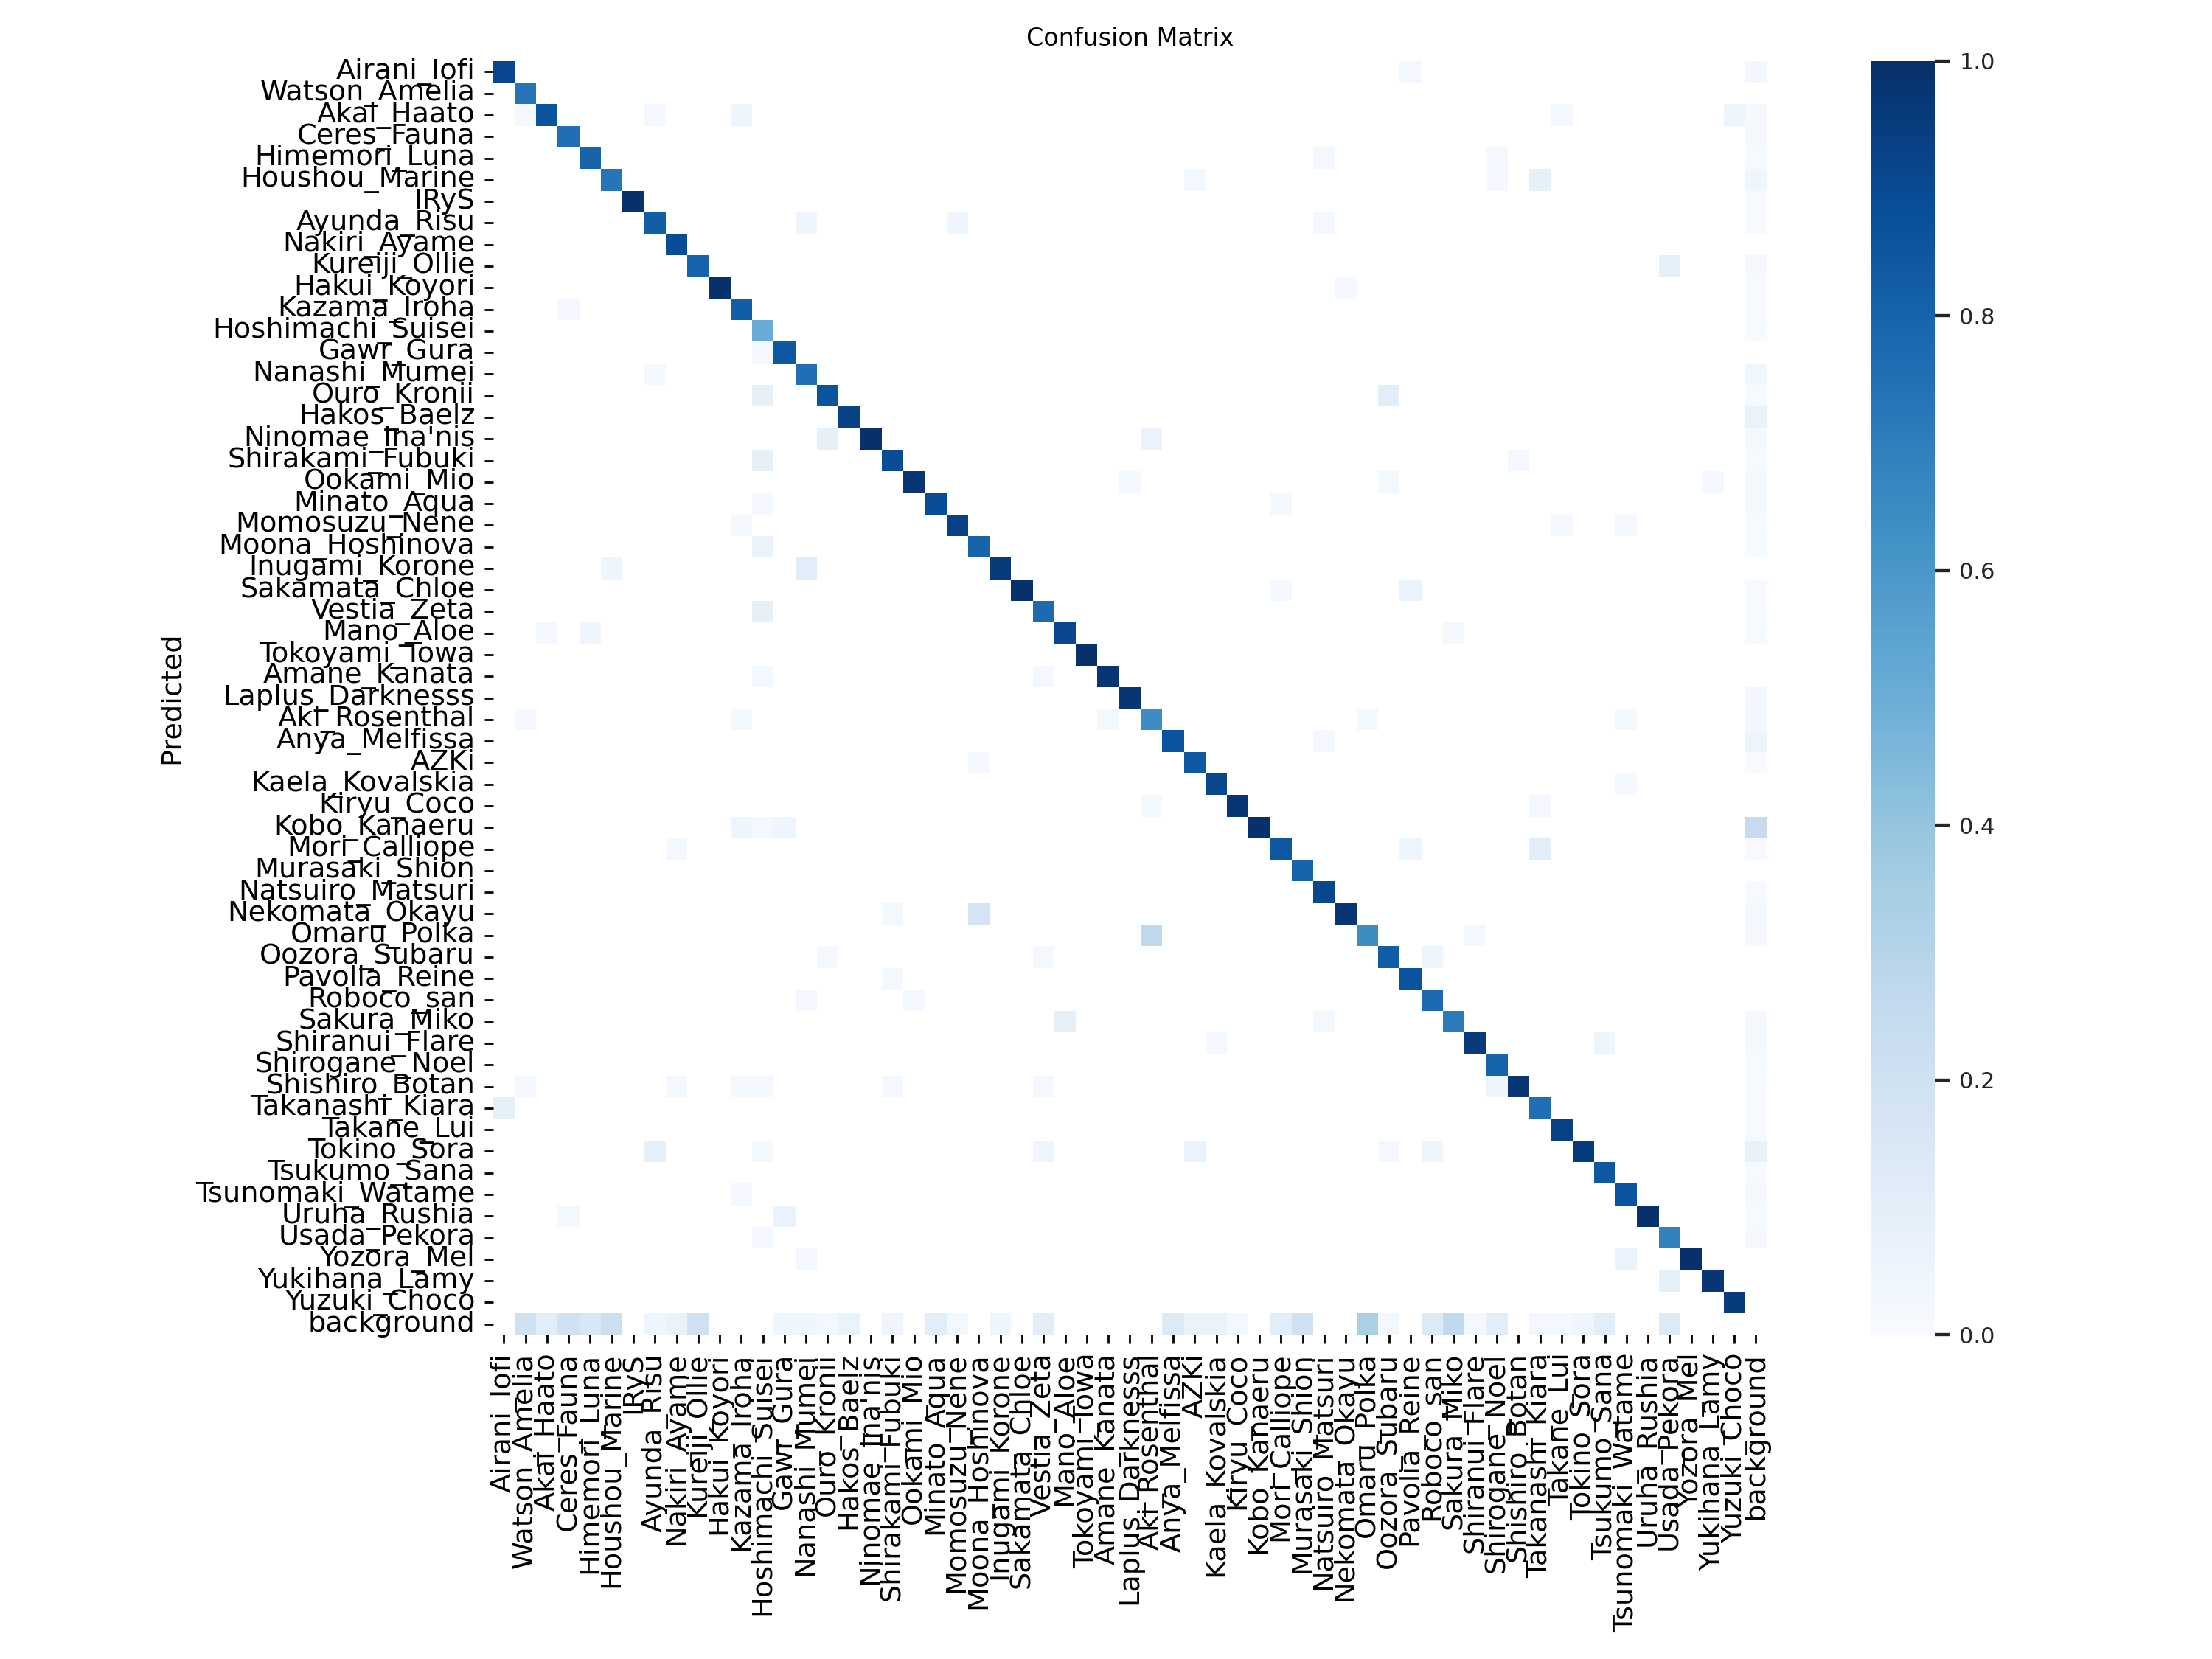
\includegraphics[width=1\textwidth]{images/results/confusion_matrix.png}
    \end{subfigure}
    \hfill
    \begin{subfigure}{1\textwidth}
        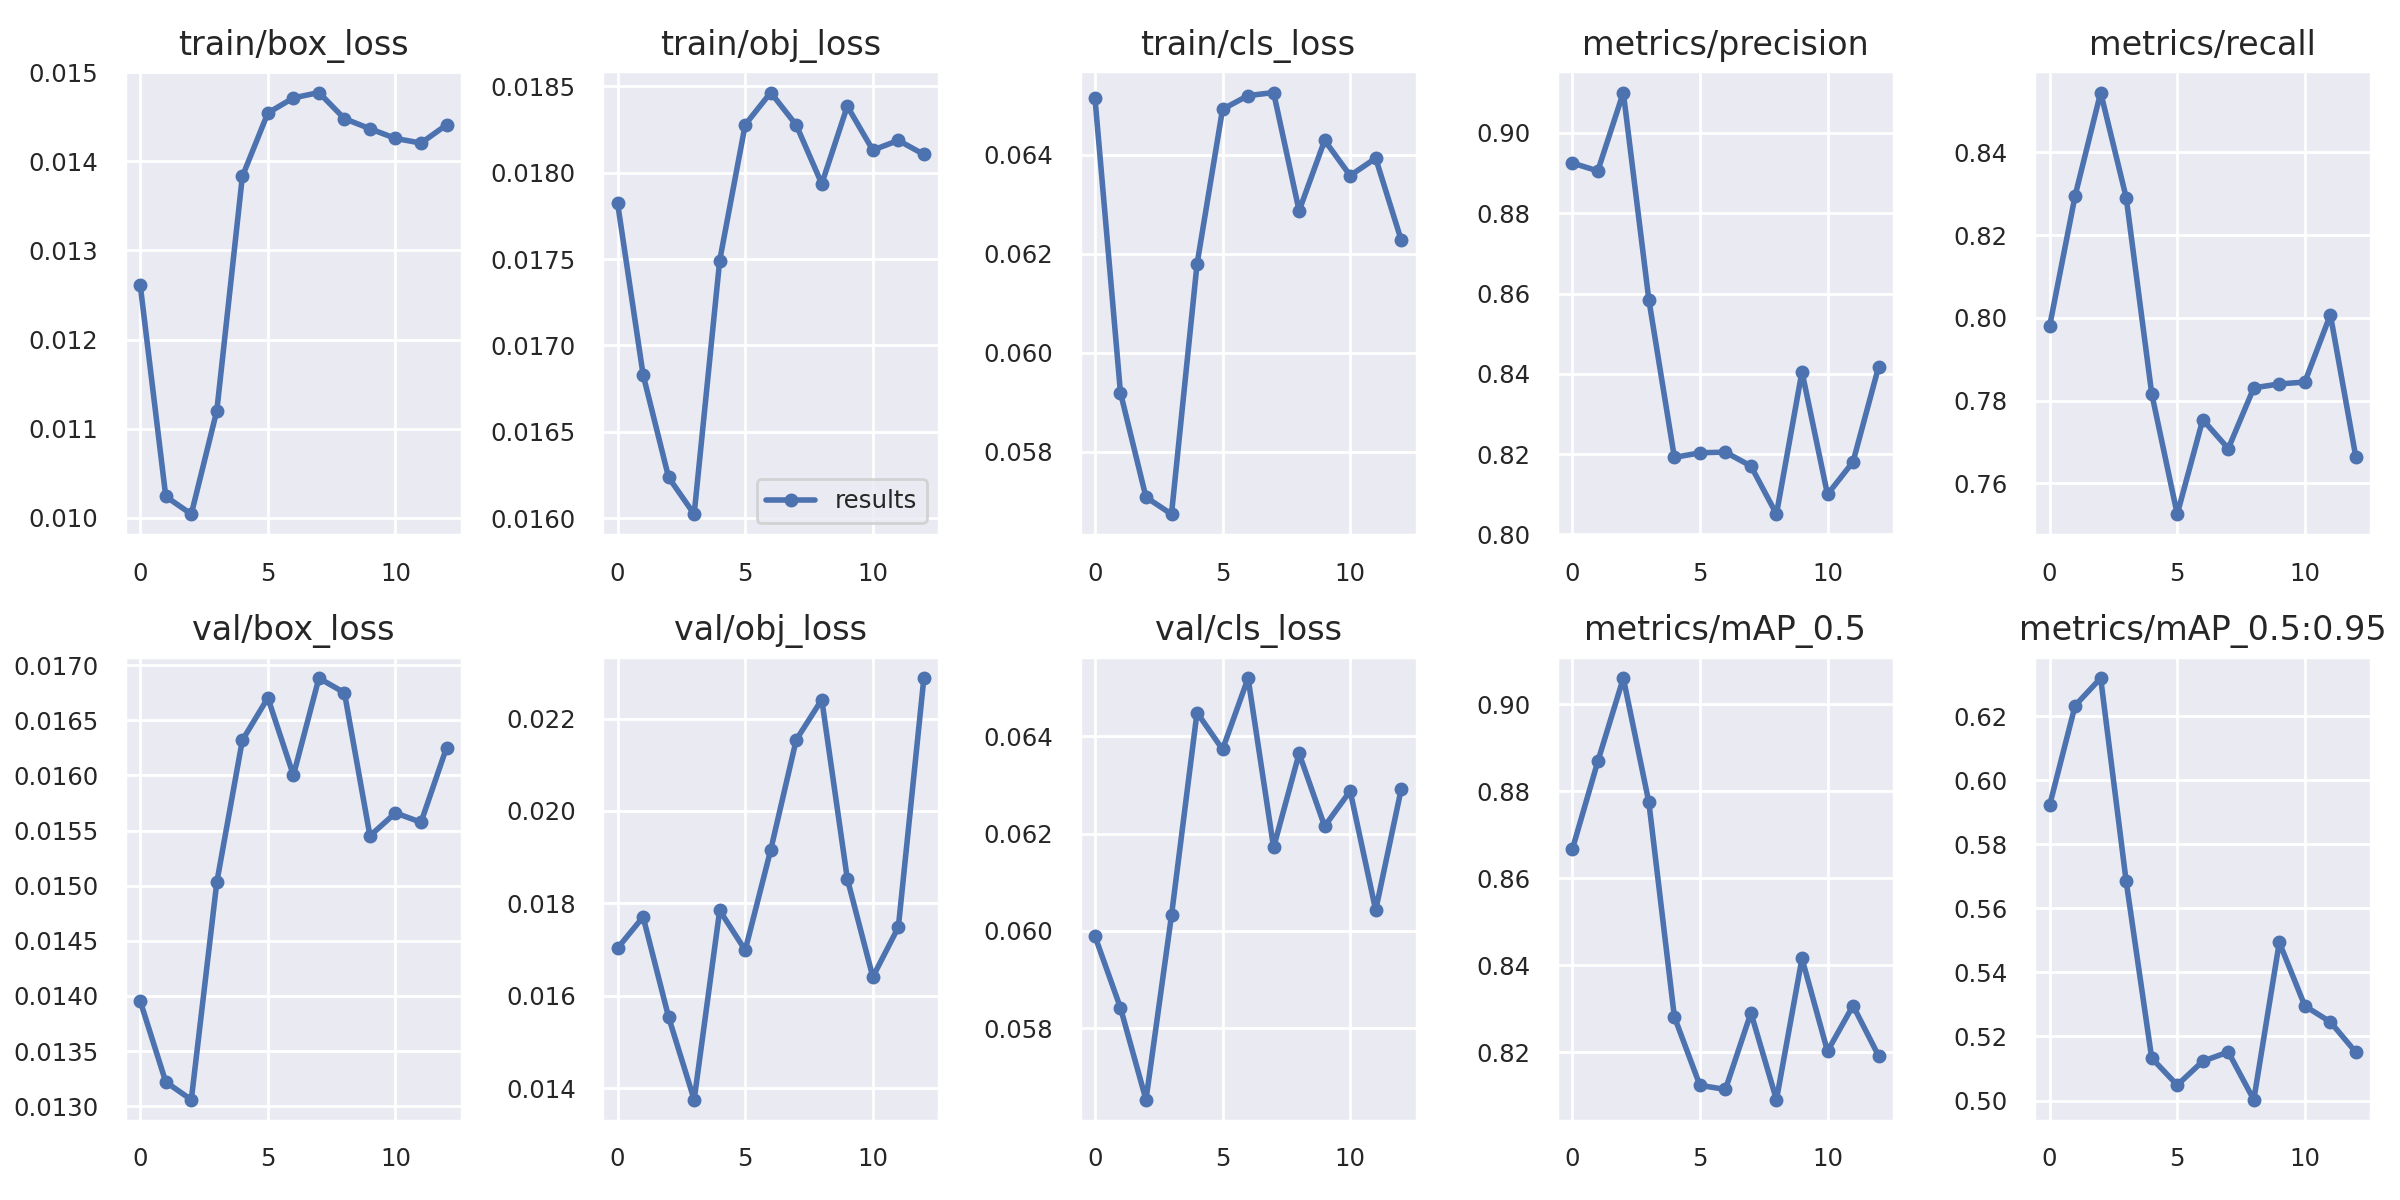
\includegraphics[width=1\textwidth]{images/results/results.png}
    \end{subfigure}
    \hfill
    \caption{Results (cont.)}
    \label{fig:result3}
\end{figure}
    \begin{figure}[H]
    \centering
    \begin{subfigure}{1\textwidth}
    \begin{center}
        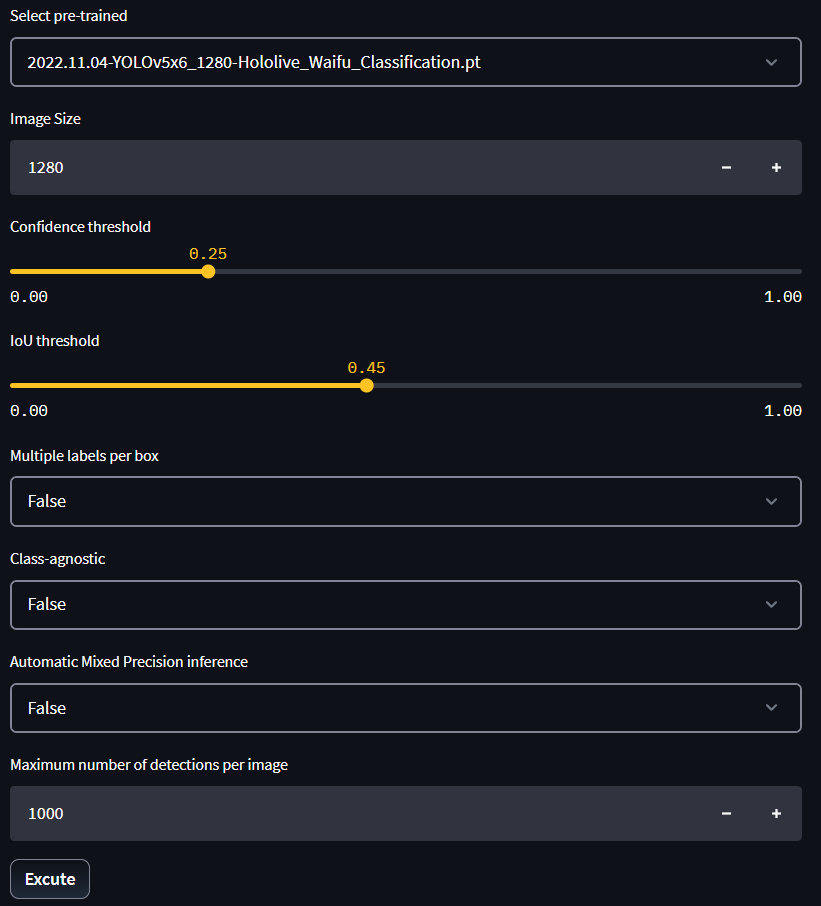
\includegraphics[width=0.66\textwidth]{images/web/PredictConfiguration.png}
        \end{center}
    \end{subfigure}
    \hfill
    \begin{subfigure}{1\textwidth}
    \begin{center}
        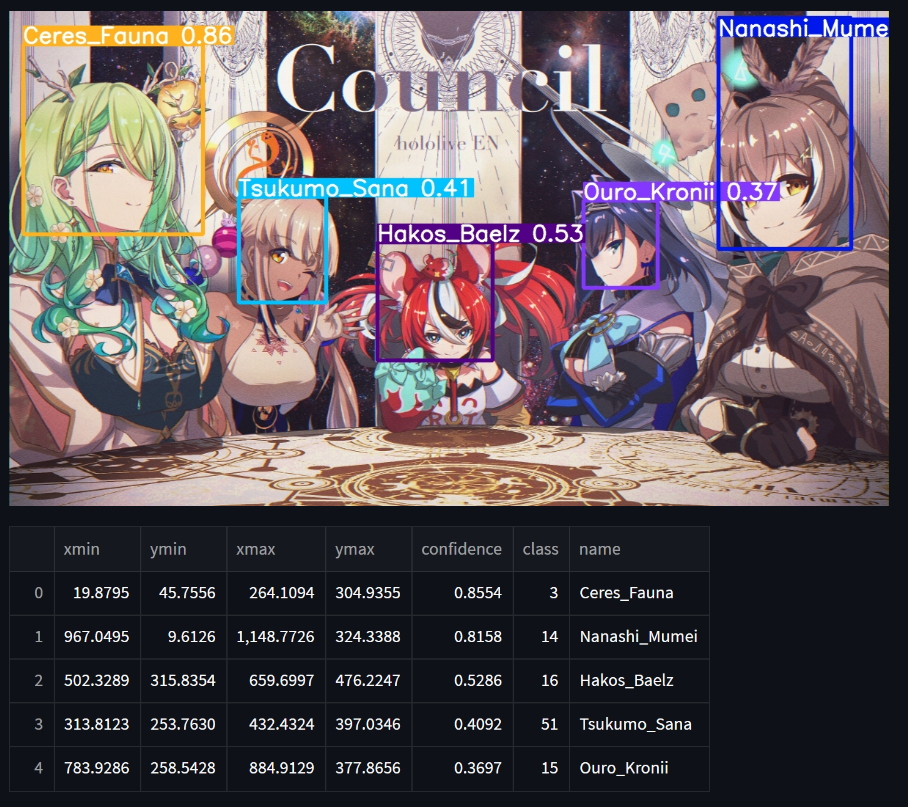
\includegraphics[width=0.66\textwidth]{images/web/SampleOutput.png}
        \end{center}
    \end{subfigure}
    \hfill
    \caption{Hololive Waifu Classification Web Application}
    \label{fig:WebApp}
\end{figure}
    \label{Table Hyperparameters}
\begin{table}
    \caption{Hyperparameters}
    \centering
    \begin{tabular}{ | m{7.5em} | m{4em} | m{4em} | 
 m{4em}| m{4em} | m{16em} |} 
        \hline
            \centering\textbf{Variable} & 
            \centering\textbf{High} & 
            \centering\textbf{Medium} & 
            \centering\textbf{Low} & 
            \centering\textbf{Evolved} &
            \centering\textbf{Description}
            \tabularnewline
        \hline
            \texttt{lr0} & 
            \centering\texttt{0.01} & 
            \centering\texttt{0.01} & 
            \centering\texttt{0.01} & 
            \centering\texttt{0.0087} &
            \texttt{Initial learning rate}
            \tabularnewline
        \hline
            \texttt{lrf} & 
            \centering\texttt{0.1} & 
            \centering\texttt{0.1} & 
            \centering\texttt{0.01} & 
            \centering\texttt{0.01236} &
            \texttt{Final OneCycleLR learning rate}
            \tabularnewline
        \hline
            \texttt{momentum} & 
            \centering\texttt{0.937} & 
            \centering\texttt{0.937} & 
            \centering\texttt{0.937} & 
            \centering\texttt{0.98} &
            \texttt{SGD momentum/Adam beta1}
            \tabularnewline
        \hline
            \texttt{weight\_decay} & 
            \centering\texttt{0.0005} & 
            \centering\texttt{0.0005} & 
            \centering\texttt{0.0005} & 
            \centering\texttt{0.00049} &
            \texttt{Optimizer weight decay}
            \tabularnewline
        \hline
            \texttt{warmup\_epochs} & 
            \centering\texttt{3.0} & 
            \centering\texttt{3.0} & 
            \centering\texttt{3.0} & 
            \centering\texttt{4.0047} &
            \texttt{Warmup epochs}
            \tabularnewline
        \hline
            \texttt{warmup\_momentum} & 
            \centering\texttt{0.8} & 
            \centering\texttt{0.8} & 
            \centering\texttt{0.8} & 
            \centering\texttt{0.71428} &
            \texttt{Warmup initial momentum}
            \tabularnewline
        \hline
            \texttt{warmup\_bias\_lr} & 
            \centering\texttt{0.1} & 
            \centering\texttt{0.1} & 
            \centering\texttt{0.1} & 
            \centering\texttt{0.10209} &
            \texttt{Warmup initial bias learning rate}
            \tabularnewline
        \hline
            \texttt{box} & 
            \centering\texttt{0.05} & 
            \centering\texttt{0.05} & 
            \centering\texttt{0.05} & 
            \centering\texttt{0.03328} &
            \texttt{Box loss gain}
            \tabularnewline
        \hline
            \texttt{cls} & 
            \centering\texttt{0.3} & 
            \centering\texttt{0.3} & 
            \centering\texttt{0.5} & 
            \centering\texttt{0.56975} &
            \texttt{Class loss gain}
            \tabularnewline
        \hline
            \texttt{cls\_pw} & 
            \centering\texttt{1.0} & 
            \centering\texttt{1.0} & 
            \centering\texttt{1.0} & 
            \centering\texttt{1.4206} &
            \texttt{Class BCELoss positive weight}
            \tabularnewline
        \hline
            \texttt{obj} & 
            \centering\texttt{0.7} & 
            \centering\texttt{0.7} & 
            \centering\texttt{1.0} & 
            \centering\texttt{0.85607} &
            \texttt{Object loss gain, scale with pixels}
            \tabularnewline
        \hline
            \texttt{obj\_pw} & 
            \centering\texttt{1.0} & 
            \centering\texttt{1.0} & 
            \centering\texttt{1.0} & 
            \centering\texttt{0.84047} &
            \texttt{Object BCELoss positive weight}
            \tabularnewline
        \hline
            \texttt{iou\_t} & 
            \centering\texttt{0.2} & 
            \centering\texttt{0.2} & 
            \centering\texttt{0.2} & 
            \centering\texttt{0.2} &
            \texttt{IoU training threshold}
            \tabularnewline
        \hline
            \texttt{anchor\_t} & 
            \centering\texttt{4.0} & 
            \centering\texttt{4.0} & 
            \centering\texttt{4.0} & 
            \centering\texttt{3.1175} &
            \texttt{Anchor with multiple threshold}
            \tabularnewline
        \hline
            \texttt{anchors} & 
            \centering\texttt{3.0} & 
            \centering\texttt{3.0} & 
            \centering\texttt{3.0} & 
            \centering\texttt{3.5689} &
            \texttt{Anchors per output layer (0 to ignore)}
            \tabularnewline
        \hline
            \texttt{fl\_gamma} & 
            \centering\texttt{0.0} & 
            \centering\texttt{0.0} & 
            \centering\texttt{0.0} & 
            \centering\texttt{0.0} &
            \texttt{Focal loss gamma}
            \tabularnewline
        \hline
            \texttt{hsv\_h} & 
            \centering\texttt{0.015} & 
            \centering\texttt{0.015} & 
            \centering\texttt{0.015} & 
            \centering\texttt{0.01316} &
            \texttt{Image HSV-Hue augmentation}
            \tabularnewline
        \hline
            \texttt{hsv\_s} & 
            \centering\texttt{0.7} & 
            \centering\texttt{0.7} & 
            \centering\texttt{0.7} & 
            \centering\texttt{0.68962} &
            \texttt{Image HSV-Saturation augmentation}
            \tabularnewline
        \hline
            \texttt{hsv\_v} & 
            \centering\texttt{0.4} & 
            \centering\texttt{0.4} & 
            \centering\texttt{0.4} & 
            \centering\texttt{0.59337} &
            \texttt{Image HSV-Value augmentation}
            \tabularnewline
        \hline
            \texttt{degrees} & 
            \centering\texttt{0.0} & 
            \centering\texttt{0.0} & 
            \centering\texttt{0.0} & 
            \centering\texttt{0.0} &
            \texttt{Image rotation}
            \tabularnewline
        \hline
            \texttt{translate} & 
            \centering\texttt{0.1} & 
            \centering\texttt{0.1} & 
            \centering\texttt{0.1} & 
            \centering\texttt{0.11811} &
            \texttt{Image translation}
            \tabularnewline
        \hline
            \texttt{scale} & 
            \centering\texttt{0.9} & 
            \centering\texttt{0.9} & 
            \centering\texttt{0.5} & 
            \centering\texttt{0.35226} &
            \texttt{Image scale}
            \tabularnewline
        \hline
            \texttt{shear} & 
            \centering\texttt{0.0} & 
            \centering\texttt{0.0} & 
            \centering\texttt{0.0} & 
            \centering\texttt{0.0} &
            \texttt{Image shear}
            \tabularnewline
        \hline
            \texttt{perspective} & 
            \centering\texttt{0.0} & 
            \centering\texttt{0.0} & 
            \centering\texttt{0.0} & 
            \centering\texttt{0.0} &
            \texttt{Image perspective, range [0, 0.001]}
            \tabularnewline
        \hline
            \texttt{flipud} & 
            \centering\texttt{0.0} & 
            \centering\texttt{0.0} & 
            \centering\texttt{0.0} & 
            \centering\texttt{0.0} &
            \texttt{Probability image flip up-down}
            \tabularnewline
        \hline
            \texttt{fliplr} & 
            \centering\texttt{0.5} & 
            \centering\texttt{0.5} & 
            \centering\texttt{0.5} & 
            \centering\texttt{0.5} &
            \texttt{Probability image flip left-right}
            \tabularnewline
        \hline
            \texttt{mosaic} & 
            \centering\texttt{1.0} & 
            \centering\texttt{1.0} & 
            \centering\texttt{1.0} & 
            \centering\texttt{0.91958} &
            \texttt{Probability image mosaic}
            \tabularnewline
        \hline
            \texttt{mixup} & 
            \centering\texttt{0.1} & 
            \centering\texttt{0.1} & 
            \centering\texttt{0.0} & 
            \centering\texttt{0.0} &
            \texttt{Probability image mixup}
            \tabularnewline
        \hline
            \texttt{copy\_paste} & 
            \centering\texttt{0.1} & 
            \centering\texttt{0.0} & 
            \centering\texttt{0.0} & 
            \centering\texttt{0.0} &
            \texttt{Probability segment copy-paste}
            \tabularnewline
        \hline
    \end{tabular}
    \label{table:Hyperparameters}
\end{table}

    \label{Table Labels Distribution}
\begin{table}
    \caption{\label{LabelDistribution}Label distribution.}
    \begin{center}
        \begin{tabular}{ | m{3.5em} | m{9em}| m{3.8em} | m{6em} | m{6em}| m{6em} |  m{6em} | } 
            \hline
                \centering\textbf{Index} & 
                \centering\textbf{Classes} & 
                \centering\textbf{Origin} & 
                \centering\textbf{Train Split} & 
                \centering\textbf{Train Aug} & 
                \centering\textbf{Val Split} & 
                \centering\textbf{Val Aug}
                \tabularnewline
            \hline              
                \centering 0 & 
                \texttt{Airani\_Iofi} &
                \centering 79 &  
                \centering 41 & 
                \centering 164 & 
                \centering 9 &
                \centering 36 
                \tabularnewline
            \hline                   
                \centering 1 & 
                \texttt{Watson\_Amelia} &
                \centering 145 &  
                \centering 41 & 
                \centering 164 & 
                \centering 9 &
                \centering 36
                \tabularnewline
            \hline
                \centering 2 & 
                \texttt{Akai\_Haato} &
                \centering 63 &  
                \centering 41 & 
                \centering 164 & 
                \centering 9 &
                \centering 36
                \tabularnewline
            \hline   
                \centering 3 & 
                \texttt{Ceres\_Fauna} &
                \centering 200 &  
                \centering 41 & 
                \centering 164 & 
                \centering 9 &
                \centering 36
                \tabularnewline
            \hline
                \centering 4 & 
                \texttt{Himemori\_Luna} &
                \centering 80 &  
                \centering 41 & 
                \centering 164 & 
                \centering 9 &
                \centering 36
                \tabularnewline
            \hline
                \centering 5 & 
                \texttt{Houshou\_Marine} &
                \centering 78 &  
                \centering 41 & 
                \centering 164 & 
                \centering 9 &
                \centering 36
                \tabularnewline
            \hline
                \centering 6 & 
                \texttt{Irys} &
                \centering 54 &  
                \centering 41 & 
                \centering 164 & 
                \centering 9 &
                \centering 36
                \tabularnewline
            \hline
        \end{tabular}
    \end{center}
    \label{table:LabelDistribution}
\end{table}
\begin{table}
    \caption{\label{LabelDistribution1}Label distribution (cont).}
    \begin{center}
        \begin{tabular}{ | m{3.5em} | m{9em}| m{3.8em} | m{6em} | m{6em}| m{6em} |  m{6em} | } 
            \hline
                \centering\textbf{Index} & 
                \centering\textbf{Classes} & 
                \centering\textbf{Origin} & 
                \centering\textbf{Train Split} & 
                \centering\textbf{Train Aug} & 
                \centering\textbf{Val Split} & 
                \centering\textbf{Val Aug}
                \tabularnewline
            \hline
                \centering 7 & 
                \texttt{Ayunda\_Risu} &
                \centering 61 &  
                \centering 41 & 
                \centering 164 & 
                \centering 9 &
                \centering 36
                \tabularnewline
            \hline
                \centering 8 & 
                \texttt{Nakiri\_Ayame} &
                \centering 67 &  
                \centering 41 & 
                \centering 164 & 
                \centering 9 &
                \centering 36
                \tabularnewline
            \hline
                \centering 9 & 
                \texttt{Kureiji\_Olie} &
                \centering 58 &  
                \centering 41 & 
                \centering 164 & 
                \centering 9 &
                \centering 36
                \tabularnewline
            \hline
                \centering 10 & 
                \texttt{Hakui\_Koyori} &
                \centering 56 &  
                \centering 41 & 
                \centering 164 & 
                \centering 9 &
                \centering 36
                \tabularnewline
            \hline
                \centering 11 & 
                \texttt{Kazama\_Iroha} &
                \centering 135 &  
                \centering 41 & 
                \centering 164 & 
                \centering 9 &
                \centering 36
                \tabularnewline
            \hline
                \centering 12 & 
                \texttt{Hoshimachi\_Suisei} &
                \centering 114 &  
                \centering 41 & 
                \centering 164 & 
                \centering 9 &
                \centering 36
                \tabularnewline
            \hline
                \centering 13 & 
                \texttt{Gawr\_Gura} &
                \centering 68 &  
                \centering 41 & 
                \centering 164 & 
                \centering 9 &
                \centering 36
                \tabularnewline
            \hline
                \centering 14 & 
                \texttt{Nanashi\_Mumei} &
                \centering 157 &  
                \centering 41 & 
                \centering 164 & 
                \centering 9 &
                \centering 36
                \tabularnewline
            \hline
                \centering 15 & 
                \texttt{Ouro\_Kronii} &
                \centering 75 &  
                \centering 41 & 
                \centering 164 & 
                \centering 9 &
                \centering 36
                \tabularnewline
            \hline
                \centering 16 & 
                \texttt{Hakos\_Baelz} &
                \centering 89 &  
                \centering 41 & 
                \centering 164 & 
                \centering 9 &
                \centering 36
                \tabularnewline
            \hline
                \centering 17 & 
                \texttt{Ninomae\_Ina'nis} &
                \centering 61 &  
                \centering 41 & 
                \centering 164 & 
                \centering 9 &
                \centering 36
                \tabularnewline
            \hline
                \centering 18 & 
                \texttt{Shirakami\_Fubiki} &
                \centering 64 &  
                \centering 41 & 
                \centering 164 & 
                \centering 9 &
                \centering 36
                \tabularnewline
            \hline
                \centering 19 & 
                \texttt{Ookami\_Mio} &
                \centering 62 &  
                \centering 41 & 
                \centering 164 & 
                \centering 9 &
                \centering 36
                \tabularnewline
            \hline
                \centering 20 & 
                \texttt{Minato\_Aqua} &
                \centering 72 &  
                \centering 41 & 
                \centering 164 & 
                \centering 9 &
                \centering 36
                \tabularnewline
            \hline
                \centering 21 & 
                \texttt{Momosuzu\_Nene} &
                \centering 60 &  
                \centering 41 & 
                \centering 164 & 
                \centering 9 &
                \centering 36
                \tabularnewline
            \hline
                \centering 22 & 
                \texttt{Moona\_Hoshinova} &
                \centering 58 &  
                \centering 41 & 
                \centering 164 & 
                \centering 9 &
                \centering 36
                \tabularnewline
            \hline
                \centering 23 & 
                \texttt{Inugami\_Korone} &
                \centering 57 &  
                \centering 41 & 
                \centering 164 & 
                \centering 9 &
                \centering 36
                \tabularnewline
            \hline
                \centering 24 & 
                \texttt{Sakamata\_Chloe} &
                \centering 61 &  
                \centering 41 & 
                \centering 164 & 
                \centering 9 &
                \centering 36
                \tabularnewline
            \hline
                \centering 25 & 
                \texttt{Vestia\_Zeta} &
                \centering 50 &  
                \centering 41 & 
                \centering 164 & 
                \centering 8 &
                \centering 32
                \tabularnewline
            \hline
                \centering 26 & 
                \texttt{Mano\_Aloe} &
                \centering 54 &  
                \centering 41 & 
                \centering 164 & 
                \centering 9 &
                \centering 36
                \tabularnewline
            \hline
                \centering 27 & 
                \texttt{Tokoyami\_Towa} &
                \centering 67 &  
                \centering 41 & 
                \centering 164 & 
                \centering 9 &
                \centering 36
                \tabularnewline
            \hline
                \centering 28 & 
                \texttt{Amane\_Kanata} &
                \centering 76 &  
                \centering 41 & 
                \centering 164 & 
                \centering 9 &
                \centering 36
                \tabularnewline
            \hline
                \centering 29 & 
                \texttt{Laplus\_Darknesss} &
                \centering 67 &  
                \centering 41 & 
                \centering 164 & 
                \centering 9 &
                \centering 36
                \tabularnewline
            \hline
                \centering 30 & 
                \texttt{Aki\_Rosenthal} &
                \centering 52 &  
                \centering 41 & 
                \centering 164 & 
                \centering 9 &
                \centering 36
                \tabularnewline
            \hline
                \centering 31 & 
                \texttt{Anya\_Melfissa} &
                \centering 60 &  
                \centering 41 & 
                \centering 164 & 
                \centering 9 &
                \centering 36
                \tabularnewline
            \hline
                \centering 32 & 
                \texttt{AZKI} &
                \centering 56 &  
                \centering 41 & 
                \centering 164 & 
                \centering 9 &
                \centering 36
                \tabularnewline
            \hline
                \centering 33 & 
                \texttt{Kaela\_Kovalskia} &
                \centering 69 &  
                \centering 41 & 
                \centering 164 & 
                \centering 9 &
                \centering 36
                \tabularnewline
            \hline
                \centering 34 & 
                \texttt{Kiryu\_Coco} &
                \centering 51 &  
                \centering 41 & 
                \centering 164 & 
                \centering 9 &
                \centering 36
                \tabularnewline
            \hline
                \centering 35 & 
                \texttt{Kobo\_Kanaeru} &
                \centering 51 &  
                \centering 41 & 
                \centering 164 & 
                \centering 9 &
                \centering 36
                \tabularnewline
            \hline
                \centering 36 & 
                \texttt{Mori\_Calliope} &
                \centering 81 &  
                \centering 41 & 
                \centering 164 & 
                \centering 9 &
                \centering 36
                \tabularnewline
            \hline
                \centering 37 & 
                \texttt{Murasaki\_Shion} &
                \centering 53 &  
                \centering 41 & 
                \centering 164 & 
                \centering 6 &
                \centering 24
                \tabularnewline
            \hline
                \centering 38 & 
                \texttt{Natsuiro\_Matsuri} &
                \centering 65 &  
                \centering 41 & 
                \centering 164 & 
                \centering 9 &
                \centering 36
                \tabularnewline
            \hline
                \centering 39 & 
                \texttt{Nekomata\_Okayu} &
                \centering 54 &  
                \centering 41 & 
                \centering 164 & 
                \centering 9 &
                \centering 36
                \tabularnewline
            \hline
                \centering 40 & 
                \texttt{Omaru\_Polka} &
                \centering 51 &  
                \centering 41 & 
                \centering 164 & 
                \centering 9 &
                \centering 36
                \tabularnewline
            \hline
                \centering 41 & 
                \texttt{Oozora\_Subaru} &
                \centering 74 &  
                \centering 41 & 
                \centering 164 & 
                \centering 9 &
                \centering 36
                \tabularnewline
            \hline
                \centering 42 & 
                \texttt{Pavolia\_Reine} &
                \centering 61 &  
                \centering 41 & 
                \centering 164 & 
                \centering 9 &
                \centering 36
                \tabularnewline
            \hline
                \centering 43 & 
                \texttt{Roboco\_san} &
                \centering 75 &  
                \centering 41 & 
                \centering 164 & 
                \centering 9 &
                \centering 36
                \tabularnewline
            \hline
                \centering 44 & 
                \texttt{Sakura\_Miko} &
                \centering 74 &  
                \centering 41 & 
                \centering 164 & 
                \centering 9 &
                \centering 36
                \tabularnewline
            \hline
                \centering 45 & 
                \texttt{Shiranui\_Flare} &
                \centering 67 &  
                \centering 41 & 
                \centering 164 & 
                \centering 9 &
                \centering 36
                \tabularnewline
            \hline
            \centering 46 & 
                \texttt{Shirogane\_Noel} &
                \centering 75 &  
                \centering 41 & 
                \centering 164 & 
                \centering 9 &
                \centering 36
                \tabularnewline
            \hline
                \centering 47 & 
                \texttt{Shishiro\_Botan} &
                \centering 63 &  
                \centering 41 & 
                \centering 164 & 
                \centering 9 &
                \centering 36
                \tabularnewline
            \hline
                \centering 48 & 
                \texttt{Takanashi\_Kiara} &
                \centering 97 &  
                \centering 41 & 
                \centering 164 & 
                \centering 9 &
                \centering 36
                \tabularnewline
            \hline
                \centering 49 & 
                \texttt{Takane\_Lui} &
                \centering 65 &  
                \centering 41 & 
                \centering 164 & 
                \centering 9 &
                \centering 36
                \tabularnewline
            \hline
            \centering 50 & 
                \texttt{Tokino\_Sora} &
                \centering 79 &  
                \centering 41 & 
                \centering 164 & 
                \centering 9 &
                \centering 36
                \tabularnewline
            \hline
                \centering 51 & 
                \texttt{Tsukumo\_Sana} &
                \centering 58 &  
                \centering 41 & 
                \centering 164 & 
                \centering 9 &
                \centering 36
                \tabularnewline
            \hline
                \centering 52 & 
                \texttt{Tsunomaki\_Watame} &
                \centering 61 &  
                \centering 41 & 
                \centering 164 & 
                \centering 9 &
                \centering 36
                \tabularnewline
            \hline
                \centering 53 & 
                \texttt{Uruha\_Rushia} &
                \centering 76 &  
                \centering 41 & 
                \centering 164 & 
                \centering 9 &
                \centering 36
                \tabularnewline
            \hline
                \centering 54 & 
                \texttt{Usada\_Pekora} &
                \centering 60 &  
                \centering 41 & 
                \centering 164 & 
                \centering 9 &
                \centering 36
                \tabularnewline
            \hline
                \centering 55 & 
                \texttt{Yozora\_Mel} &
                \centering 50 &  
                \centering 41 & 
                \centering 164 & 
                \centering 7 &
                \centering 28
                \tabularnewline
            \hline

                \centering 56 & 
                \texttt{Yukihana\_Lamy} &
                \centering 60 &  
                \centering 41 & 
                \centering 164 & 
                \centering 9 &
                \centering 36
                \tabularnewline
            \hline
                \centering 57 & 
                \texttt{Yuzuki\_Choco} &
                \centering 73 &  
                \centering 41 & 
                \centering 164 & 
                \centering 9 &
                \centering 36
                \tabularnewline
            \hline
            \end{tabular}            
    \end{center}
    \label{table:LabelDistribution1}
\end{table}
    \label{Table Dataset Information}
\begin{table*}[bp]
    \caption{\label{DatasetInformation}Dataset information.} 
    \begin{center}
        \begin{tabular}{ | m{7em} | m{7em} | m{7em}| m{7em} | } 
            \hline
                \centering\textbf{Data} & 
                \centering\textbf{Training} & 
                \centering\textbf{Validating} & 
                \centering\textbf{Sum}
                \tabularnewline
            \hline
                \centering\textbf{Split} &
                \centering 1981 & 
                \centering 483 & 
                \centering 2464
                \tabularnewline
            \hline
                \centering\textbf{Augmentation} &
                \centering 7924 & 
                \centering 1932 & 
                \centering 9856
                \tabularnewline
            \hline
                \centering\textbf{Background} &
                \centering 1033 & 
                \centering 268 & 
                \centering 1301
                \tabularnewline
            \hline
                \centering\textbf{Sum} &  
                \centering 10938 & 
                \centering 2683 & 
                \centering 13621
                \tabularnewline
            \hline
        \end{tabular}  
    \end{center}
    \label{table:DatasetInformation}
\end{table*}
    \begin{table}
    \caption{\label{Configuration}Configuration} 
    \begin{center}
        \begin{tabular}{ | m{8em} | m{5em} | m{5em} | 
 m{5em}| m{15em} | } 
            \hline
                \centering\textbf{Argument} & 
                \centering\textbf{Default} & 
                \centering\textbf{Evolve} & 
                \centering\textbf{Train} & 
                \centering\textbf{Description}
                \tabularnewline
            \hline
                \texttt{epochs} &
                \centering 100 & 
                \centering 10 & 
                \centering 1000 & 
                \texttt{Total training epochs}
                \tabularnewline
            \hline
                \texttt{batch\_size} &
                \centering 16 & 
                \centering -1 & 
                \centering -1 & 
                \texttt{Total batch size for all GPUs, -1 for autobatch}
                \tabularnewline
            \hline
                \texttt{imgsz} &
                \centering 640 & 
                \centering 1280 & 
                \centering 1280 & 
                \texttt{Image size}
                \tabularnewline
            \hline
                \texttt{rect} &
                \centering\texttt{false} & 
                \centering\texttt{false} & 
                \centering\texttt{false} & 
                \texttt{Forces rectangular image training}
                \tabularnewline
            \hline
                \texttt{nosave} &
                \centering\texttt{false} & 
                \centering\texttt{false} & 
                \centering\texttt{false} & 
                \texttt{Only save final checkpoint}
                \tabularnewline
            \hline
                \texttt{noval} &
                \centering\texttt{false} & 
                \centering\texttt{false} & 
                \centering\texttt{false} & 
                \texttt{Only validate final epoch}
                \tabularnewline
            \hline
                \texttt{noautoanchor} &
                \centering\texttt{false} & 
                \centering\texttt{false} & 
                \centering\texttt{false} & 
                \texttt{Disable AutoAnchor}
                \tabularnewline
            \hline
                \texttt{noplots} &
                \centering\texttt{false} & 
                \centering\texttt{false} & 
                \centering\texttt{false} & 
                \texttt{Save no plot files}
                \tabularnewline
            \hline
                \texttt{evolve} &
                \centering\texttt{null} & 
                \centering\texttt{300} & 
                \centering\texttt{null} & 
                \texttt{Evolve hyperparameters for x generations}
                \tabularnewline
            \hline
                \texttt{bucket} &
                \centering\texttt{''} & 
                \centering\texttt{''} & 
                \centering\texttt{''} & 
                \texttt{Gsutil bucket}
                \tabularnewline
            \hline
                \texttt{cache} &
                \centering\texttt{null} & 
                \centering\texttt{'ram'} & 
                \centering\texttt{'ram'} & 
                \texttt{image --cache ram/disk}
                \tabularnewline
            \hline
                \texttt{image-weights} &
                \centering\texttt{false} & 
                \centering\texttt{false} & 
                \centering\texttt{true} & 
                \texttt{Use weighted image selection for training}
                \tabularnewline
            \hline
                \texttt{device} &
                \centering\texttt{''} & 
                \centering\texttt{''} & 
                \centering\texttt{''} & 
                \texttt{Cuda device, i.e. 0 or 0,1,2,3 or cpu}
                \tabularnewline
            \hline
                \texttt{multi-scale} &
                \centering\texttt{false} & 
                \centering\texttt{false} & 
                \centering\texttt{true} & 
                \texttt{Vary img-size +/- 50\%\%}
                \tabularnewline
            \hline
                \texttt{single-cls} &
                \centering\texttt{false} & 
                \centering\texttt{false} & 
                \centering\texttt{false} & 
                \texttt{Train multi-class data as single-class}
                \tabularnewline
            \hline
                \texttt{optimizer} &
                \centering\texttt{'SGD'} & 
                \centering\texttt{'AdamW'} & 
                \centering\texttt{'SGD'} & 
                \texttt{Optimizer in ['SGD', 'Adam', 'AdamW']}
                \tabularnewline
            \hline
                \texttt{exist-ok} &
                \centering\texttt{false} & 
                \centering\texttt{true} & 
                \centering\texttt{true} & 
                \texttt{Existing project/name ok, do not increment}
                \tabularnewline
            \hline
                \texttt{quad} &
                \centering\texttt{false} & 
                \centering\texttt{false} & 
                \centering\texttt{false} & 
                \texttt{Quad dataloader}
                \tabularnewline
            \hline
                \texttt{cos-lr} &
                \centering\texttt{false} & 
                \centering\texttt{false} & 
                \centering\texttt{false} & 
                \texttt{Cosine LR scheduler}
                \tabularnewline
            \hline
                \texttt{label-smoothing} &
                \centering\texttt{0.0} & 
                \centering\texttt{0.01} & 
                \centering\texttt{0.01} & 
                \texttt{Label smoothing epsilon}
                \tabularnewline
            \hline
                \texttt{patience} &
                \centering\texttt{100} & 
                \centering\texttt{100} & 
                \centering\texttt{10} & 
                \texttt{Label smoothing epsilon}
                \tabularnewline
            \hline
                \texttt{freeze} &
                \centering\texttt{[0]} & 
                \centering\texttt{[0]} & 
                \centering\texttt{[0]} & 
                \texttt{Freeze layers: backbone=10, first3=0 1 2}
                \tabularnewline
            \hline
                \texttt{save-period} &
                \centering\texttt{-1} & 
                \centering\texttt{-1} & 
                \centering\texttt{-1} & 
                \texttt{Save checkpoint every x epochs (disabled if < 1)}
                \tabularnewline
            \hline
                \texttt{seed} &
                \centering\texttt{0} & 
                \centering\texttt{0} & 
                \centering\texttt{941} & 
                \texttt{Global training seed}
                \tabularnewline
            \hline
        \end{tabular}  
    \end{center}
    \label{table:Configuration}
\end{table}
    \begin{figure}
    \begin{tikzpicture}
        \begin{axis} [
            xbar,
            width=1\linewidth,
            height=1\textheight,
            xmin=0,
            % xmax=5,
            ymin=0,
            ymax=57,
            enlarge y limits = {abs = .8}, % add 0.8 units to both sides of our y axis (top and bottom)
        ]
        \addplot coordinates {
            (79, 0)
            (145, 1)
            (63, 2)
            (200, 3)
            (80, 4)
            (78, 5)
            (54, 6)
            (61, 7)
            (67, 8)
            (58, 9)
            (56, 10)
            (135, 11)
            (114, 12)
            (68, 13)
            (157, 14)
            (75, 15)
            (89, 16)
            (61, 17)
            (64, 18)
            (62, 19)
            (72, 20)
            (60, 21)
            (58, 22)
            (57, 23)
            (61, 24)
            (50, 25)
            (54, 26)
            (67, 27)
            (76, 28)
            (67, 29)
            (52, 30)
            (60, 31)
            (56, 32)
            (69, 33)
            (51, 34)
            (51, 35)
            (81, 36)
            (53, 37)
            (65, 38)
            (54, 39)
            (51, 40)
            (74, 41)
            (61, 42)
            (75, 43)
            (74, 44)
            (67, 45)
            (75, 46)
            (63, 47)
            (97, 48)
            (65, 49)
            (79, 50)
            (58, 51)
            (61, 52)
            (76, 53)
            (60, 54)
            (50, 55)
            (60, 56)
            (73, 57)
            };
        \end{axis}
    \end{tikzpicture}
    \caption{Original dataset label distribution}
    \label{chart:Originaldatasetlabeldistribution}
\end{figure}
    \begin{figure}
    \begin{tikzpicture}
        \begin{axis} [
            xbar,
            width=1\linewidth,
            height=1\textheight,
            xmin=0,
            % xmax=5,
            ymin=0,
            ymax=57,
            enlarge y limits = {abs = .8}, % add 0.8 units to both sides of our y axis (top and bottom)
        ]
        \addplot coordinates {
            (41, 0)
            (41, 1)
            (41, 2)
            (41, 3)
            (41, 4)
            (41, 5)
            (41, 6)
            (41, 7)
            (41, 8)
            (41, 9)
            (41, 10)
            (41, 11)
            (41, 12)
            (41, 13)
            (41, 14)
            (41, 15)
            (41, 16)
            (41, 17)
            (41, 18)
            (41, 19)
            (41, 20)
            (41, 21)
            (41, 22)
            (41, 23)
            (41, 24)
            (41, 25)
            (41, 26)
            (41, 27)
            (41, 28)
            (41, 29)
            (41, 30)
            (41, 31)
            (41, 32)
            (41, 33)
            (41, 34)
            (41, 35)
            (41, 36)
            (41, 37)
            (41, 38)
            (41, 39)
            (41, 40)
            (41, 41)
            (41, 42)
            (41, 43)
            (41, 44)
            (41, 45)
            (41, 46)
            (41, 47)
            (41, 48)
            (41, 49)
            (41, 50)
            (41, 51)
            (41, 52)
            (41, 53)
            (41, 54)
            (41, 55)
            (41, 56)
            (41, 57)
            };
        \end{axis}
    \end{tikzpicture}
    \caption{Training set label distribution}
    \label{chart:Trainingsetlabeldistribution}
\end{figure}
    \begin{figure}
    \begin{tikzpicture}
        \begin{axis} [
            xbar,
            width=1\linewidth,
            height=1\textheight,
            xmin=0,
            % xmax=5,
            ymin=0,
            ymax=57,
            enlarge y limits = {abs = .8}, % add 0.8 units to both sides of our y axis (top and bottom)
        ]
        \addplot coordinates {
            (9, 0)
            (9, 1)
            (9, 2)
            (9, 3)
            (9, 4)
            (9, 5)
            (9, 6)
            (9, 7)
            (9, 8)
            (9, 9)
            (9, 10)
            (9, 11)
            (9, 12)
            (9, 13)
            (9, 14)
            (9, 15)
            (9, 16)
            (9, 17)
            (9, 18)
            (9, 19)
            (9, 20)
            (9, 21)
            (9, 22)
            (9, 23)
            (9, 24)
            (8, 25)
            (9, 26)
            (9, 27)
            (9, 28)
            (9, 29)
            (9, 30)
            (9, 31)
            (9, 32)
            (9, 33)
            (9, 34)
            (9, 35)
            (9, 36)
            (6, 37)
            (9, 38)
            (9, 39)
            (9, 40)
            (9, 41)
            (9, 42)
            (9, 43)
            (9, 44)
            (9, 45)
            (9, 46)
            (9, 47)
            (9, 48)
            (9, 49)
            (9, 50)
            (9, 51)
            (9, 52)
            (9, 53)
            (9, 54)
            (7, 55)
            (9, 56)
            (9, 57)
            };
        \end{axis}
    \end{tikzpicture}
    \caption{Validating set label distribution}
    \label{chart:Validatingsetlabeldistribution}
\end{figure}
    \clearpage
        % \clearpage
    % \end{multicols}
\end{document}